%%%%%%%%%%%%%%%%%%%%%%%%%%%%%%%%%%%%%%%%%%%%%%%%%%%%%%%%%%%%%%%%%%%%%%%%%%%%%%
%	Plantilla para Memorias y Tesis, UTFSM, Chile
%	=============================================
%
% Autor:
%       Jaime C. Rubin-de-Celis <jaime@rubin-de-celis.com>
%
% Fecha:	
%       $Date: 2016-05-28 11:05:52 -0400 (Sat, 28 May 2016) $
%
% Versión:
%       1.0
%
% Licencia:
%       Copyright (c) 2012-2016, Jaime C. Rubin-de-Celis
%       The MIT Licence
%
% Nota:
%       Las imágenes son propiedad intelectual de la UTFSM.
%
% Uso:
%       Ver archivo adjunto README.md.
%       Si todo lo demás falla, recuerde "RFM".
%
%%%%%%%%%%%%%%%%%%%%%%%%%%%%%%%%%%%%%%%%%%%%%%%%%%%%%%%%%%%%%%%%%%%%%%%%%%%%%%

\documentclass[
	12pt,			% Tamaño de fuente (11pt)
	letterpaper,	% Tamaño del papel (carta)
    oneside		% Impresión por ambos lados
]{thesis_utfsm}

\usepackage{thesis_utfsm}
\usepackage{amsmath} % Archivo de estilos 
\usepackage{subcaption}

%!TEX root = memoria.tex

%---------------------------------------------------------------------------
%%% CONFIGURACIÓN
%---------------------------------------------------------------------------
%
%%% CODIFICACIÓN DE CARACTERES
% Este documento está escrito usando caracteres Unicode (UTF8)
% Por lo que la siguiente línea es necesaria para reconocer los acentos
% y otros caracteres en español.
% Si ve caracteres extraños en el PDF (en Windows o MAC) pruebe 
% con alguna de estas líneas:
\usepackage[utf8x]{inputenc}    % *nix / Linux / MacOSX
%\usepackage[latin1]{inputenc}  % Windows (MacOSX)


\newcommand{\TheTitle}{%
    EVALUACIÓN DE MODELOS DE APRENDIZAJE AUTOMÁTICO
PARA POSICIONAMIENTO INDOOR UTILIZANDO BLUETOOTH
LOW ENERGY
}%
\newcommand{\TheAuthor}          {FELIPE IGNACIO BERRIOS TOLOZA}
\newcommand{\TheGrade}           {INGENIERO CIVIL INFORMÁTICO} % Elegir "O" ó "A"
\newcommand{\TheCity}            {SANTIAGO}
\newcommand{\TheDate}            {ABRIL 2018}
\newcommand{\TheAdvisor}         {SR. HERNÁN ASTUDILLO ROJAS}
\newcommand{\TheCoAdvisor}       {SR. RICARDO ÑANCULEF ALEGRÍA}
\newcommand{\TheScndCoAdvisor}       {SR. HERNÁN BENAVENTE CERDA}


%\newcommand{\TheScndCoAdvisor}   {SRTA. XXXXXXX XXXXXXXX X.} % Opcional

% Marca de agua, puede ser deshabilitada para impresión rápida
\insertWatermark{figures/logousm_watermark.jpg}
%---------------------------------------------------------------------------


%---------------------------------------------------------------------------
%%% No editar (¡Ver licencia!) (MIT License, 2016)
%---------------------------------------------------------------------------
\hypersetup{  
    pdfinfo={  
        Subject={Memoria Departamento de Industria, UTFSM},
        Keywords={Memoria} {Departamento de Informatica} {UTFSM},
        Producer={JCR LaTeX Templates, http://www.rubin-de-celis.com/},
        Licence={http://www.rubin-de-celis.com/LICENSE},
        pdfpagemode=FullScreen,
        pdfmenubar=false,
        pdftoolbar=false
    }  
}
\hypersetup{  
    pdfinfo={  
        Title={\TheTitle},
        Author={\TheAuthor}
    }  
}
%---------------------------------------------------------------------------              % Configuración (Título, autor, etc.)
                            % Usted debe modificar este documento
                            % para actualizar la portada.

\makeatother                % Important! (Do not delete or move!)


% Generadores de texto aleatorio (se pueden eliminar)
\usepackage{blindtext}      % automated text generation
\usepackage{lipsum}         % automated text generation


%---------------------------------------------------------------------------
%%%%%%%%%%%%%%%%%%%%%%%%%%%%%%%%%%%%%%%%%%%%%%%%%%%%%%%%%%%%
%	Documento
%%%%%%%%%%%%%%%%%%%%%%%%%%%%%%%%%%%%%%%%%%%%%%%%%%%%%%%%%%%%
\begin{document}

\pagestyle{plain}           % Headers & Footers (Roman numbers)

%---------------------------------------------------------------------------
%%%%%%%%%%%%%%%%%%%%%%%%%%%%%%%%%%%%
%	Portada
%%%%%%%%%%%%%%%%%%%%%%%%%%%%%%%%%%%%
\insertFile{portada}        % Insertar archivo 'sections/portada.tex'.

%---------------------------------------------------------------------------
%%%%%%%%%%%%%%%%%%%%%%%%%%%%%%%%%%%%
%	Preámbulo (Front Matter)
%%%%%%%%%%%%%%%%%%%%%%%%%%%%%%%%%%%%
\frontmatter                % Important! (Do not delete or move!)

%\dedicatoria{%
%    \emph{\huge A mi familia \dots}

%    \vspace*{2cm}[Puede ocupar este espacio para escribir una 
%    dedicatoria (opcional). Revise el archivo maestro
%    \inlinecode{memoria.tex}]
%}%

%\section*{(AGRADECIMIENTOS) [Título es opcional] }
%\insertFile[empty]{agradecimientos} % Insertar 'sections/agradecimientos.tex'.


\section*{RESUMEN EJECUTIVO}
\insertFile[plain]{resumen}     % Insertar 'sections/resumen.tex'.


\section*{ABSTRACT}
\insertFile[plain]{abstract}    % Insertar 'sections/abstract.tex'.

\section*{Glosario}
\insertFile[plain]{glosario}


%%% TABLA DE CONTENIDOS / FIGURAS / CUADROS
\begin{spacing}{1}      % Single space for TOC, LOF and LOT
    \tableofcontents\listoftables\listoffigures
\end{spacing}



%---------------------------------------------------------------------------
%%%%%%%%%%%%%%%%%%%%%%%%%%%%%%%%%%%%
%	Cuerpo Principal (Main Matter)
%%%%%%%%%%%%%%%%%%%%%%%%%%%%%%%%%%%%
\mainmatter             % Important! (Do not delete or move!)

\pagestyle{fancy}       % Headers & Footers (Arabic numbers)

% Incluir Capítulos
%!TEX root = ../memoria.tex

\chapter{Introducción}

Hola

%!TEX root = ../memoria.tex

\chapter{Definición del problema}

\section{Definición del problema}

En la actualidad, el sistema de posicionamiento global, GPS por sus siglas en inglés, se ha vuelto la tecnología de facto para el posicionamiento en exteriores, ya que permite una exactitud que puede alcanzar los 2 metros. El mayor problema radica en que GPS se basa en ondas con una frecuencia que habitualmente no traspasa objetos sólidos, con lo cual las señales enviadas por los múltiples satélites no traspasan algunas barreras con facilidad.

Cuando se usa tecnología GPS dentro de edificios o bajo tierra, existen muchos obstáculos e interferencia que empeoran significativamente la señal y exactitud, o simplemente las señales no pueden ser alcanzadas en el dispositivo. Con una frecuencia de 1575.42 MHz, GPS está calificado como una señal de alta frecuencia, es por ello que su longitud de onda es corta y no puede atravesar objetos macizos. 

Para realizar la aproximación de posición de un determinado dispositivo o terminal, GPS utiliza 24 satélites a unos 20.200 kilómetros de altura. Cuando un determinado dispositivo desea saber su ubicación, debe contar con al menos tres satélites en su rango de visión, y utilizando la trilateración, se obtiene una aproximación de unos pocos metros hasta inclusive unos pocos centímetros.

Entre las principales fuentes de error en la calidad de los datos de posición que afectan a GPS, se encuentran principalmente los errores propios del satélite, como por ejemplo su reloj interno, errores orbitales y errores de la configuración geométrica entre los satélites. Por otro lado, existen errores a la recepción del dispositivo, como el ruido asociado a los datos o el centro de fase de antena. Finalmente y mas relativo a este trabajo, están los llamados errores de propagación, que son asociados al medio en donde se transportan las ondas, afectando significativamente los resultados obtenidos.

Para solucionar este problema, existen los denominados indoor positioning systems (IPS), los cuales consisten en sistemas basados en redes inalámbricas, campos magnéticos, señales acústicas y otros métodos que utilizan los sensores internos de los teléfonos celulares. Algunos ejemplos de los problemas que resuelven estos sistemas son por ejemplo ayudar a encontrar tiendas dentro de un centro comercial, guiar  personas discapacitadas visualmente en instalaciones o edificios, ayudar al transporte dentro de minas subterráneas para mover materiales. También se ha planteado sistemas de rescate en donde ante una eventualidad como por ejemplo un incendio, alguien alarma al sistema y este busca la salida más cercana dentro del edificio guiando al usuario \citep{5647401}.

Las tecnologías inalámbricas se han convertido en las más prometedoras dentro de los IPS, las cuales destacan debido al auge de los smartphones y la facilidad de utilizar redes como WiFi y Bluetooth. Muchas implementaciones de IPS se han realizado para WiFi, ya que este presenta un rango mucho más grande que Bluetooth, de hasta 35 metros, sin embargo las señales en ocasiones pueden ser muy ruidosas. Bluetooth por su parte tiene un alcance en interiores de hasta 10 metros, pero con una precisión de hasta 1 metro.  Además, la última versión de Bluetooth denominada Bluetooth low energy consume significativamente menos energía que WiFi.

Las técnicas actuales de posicionamiento indoor cuentan con problemas como la reflexión en múltiples objetos como paredes, muebles o el mismo cuerpo humano. Este problema se denomina  “multi-path propagation”, y es uno de los principales causantes de error en la localización en interiores. Los métodos que confían plenamente en el indicador RSSI, el cual mide la fuerza de la señal, están sujetos a errores inherentes a la variación de las señales y al ruido.  Múltiples modelos matemáticos se utilizan para sobrellevar esta situación, entonces evaluar algoritmos que aprendan de la intensidad de las señales en cierta área es necesario para estimar de mejor manera la posición. Por lo tanto, el problema a abordar es mejorar la exactitud del posicionamiento indoor, para lo cual se utiliza técnicas de aprendizaje automático.

\section{Objetivos}

El principal objetivo de este trabajo es determinar los algoritmos de aprendizaje automático que presenten mejores resultados en términos de precisión y exactitud para posicionamiento ``indoor'' o en interiores, a partir de la experimentación en un recinto definido bajo ciertas condiciones experimentales.

\subsection{Objetivos Específicos}

\begin{itemize}
\item Evaluar calidad de las señales \textit{Bluetooth Low Energy}, tanto en precisión como exactitud.

\item Diseñar un método de mapeo para un área mediante señales RSSI (\textit{fingerprint}).

\item Comparar métodos de aprendizaje automático sobre mediciones RSSI para determinar cual posee menor error y es más exacto.

\item Identificar límites del modelo propuesto, tanto es precisión, exactitud, error, distancia de alcance las señales, y otros factores variables.

\end{itemize}

\begin{quote}
    ``\LaTeX{} es un sistema de diagramación de documentos.'' \citep{Lamport94}.
\end{quote}


\newpage


\chapter{Estado del Arte}

En los últimos años, el uso de sistemas de localización en interiores ha tomado mucha importancia en una gran cantidad de aplicaciones y contextos. En exteriores, la tecnología de facto es GPS, que sin embargo no presenta buenos resultados en interiores debido a la pobre o nula señal que es recibida en recintos cerrados o bajo tierra. A pesar de que la necesidad de posicionar o monitorear personas u objetos en interiores es alta, los avances no han sido significativos en este campo, debido a la gran cantidad de dificultades que se presentan al momento de resolver este problema como son por ejemplo propagación por múltiples caminos o \textit{Non Line of Sight} (NLoS), es decir, sin línea de visión a los diferentes emisores de señales debido a las condiciones del sistema. También se presentan otros problemas por las condiciones cambiantes del ambiente, por ejemplo, múltiples dispositivos funcionando simultáneamente, alto tránsito de personas y objetos, lo cual atenúa en gran medida las señales o la dispersión de la radiación que es un fenómeno físico frecuente en las ondas de radio.

Claramente no existe una única solución que se adapte a todos los lugares o recintos, ya que cada uno de estos tiene características únicas o en ocasiones se requiere satisfacer ciertos parámetros como por ejemplo costos, exactitud, precisión, escalabilidad, entre otros. Por lo general no es posible optimizar simultáneamente todos estos parámetros nombrados anteriormente, por lo que habitualmente se evalúan las mejores combinaciones de ellos para obtener el mejor desempeño, adaptados a una solución personalizada dependiendo del ambiente en el cual se implementa el sistema de posicionamiento.

\section{Tecnologías para posicionamiento \textit{indoor}}

Una gran cantidad de tecnologías han sido dispuestas para el desarrollo de soluciones al problema de posicionamiento en interiores. Las siguientes secciones muestran las más utilizadas y que a lo largo de múltiples estudios han presentado los mejores resultados.

\subsection{Basado en Visión}

Esta aproximación está basada en el uso de datos provistos mediante cámaras, en formato de vídeo o fotografías. Habitualmente se utilizan dos técnicas para su implementación:

\textbf{Sistemas de cámara fijos:} En este caso el ambiente es equipado con cámaras en diferentes puntos, procurando cubrir la totalidad del recinto. El objetivo entonces consiste en encontrar un objeto en movimiento capturado por una o diversas cámaras. Las características del objeto a rastrear deben ser diferenciadas, con lo cual, cuando estas características sobresalientes están presentes en alguna de las cámaras, es posible obtener la distancia relativa, y por ende, al estar fijas las cámaras, la posición también es obtenida basado en la distribución espacial dentro de las imágenes capturadas.

\textbf{Sistemas de cámaras en movimiento:} El objetivo móvil está equipado con una cámara y la localización se realiza colocando varios puntos de referencia en posiciones conocidas (y orientaciones) o extrayendo características del entorno. Si la cámara móvil detecta dos o más puntos de referencia, puede descubrir su propia posición y orientación. Para ello, el proceso de localización implica dos etapas. En la etapa fuera de línea, imágenes del ambiente se capturan en ubicaciones predefinidas y cada imagen se procesa para extraer sus características únicas para almacenarlas en una base de datos. En la etapa en línea, la cámara captura una imagen y se extraen sus características y se comparan con las características almacenadas para estimar la ubicación de la cámara.

Estas técnicas han alcanzado altos niveles de precisión, inferiores incluso a \(10^{-6} [m]\) para sistemas de alta precisión \citep{6071925}. Por otra parte, la capacidad computacional de vídeo y las altas tasas de procesamiento de datos, sumado a los nuevos algoritmos de compresión y procesamiento de imágenes, hacen de esta tecnología una de las más prometedoras. Un punto desfavorable son sus altos costos, y poca escalabilidad, sin embargo, nuevas formas de utilizar las cámaras de dispositivos móviles están siendo investigadas para desarrollar soluciones de bajo costo manteniendo la eficiencia.

Uno de los acercamientos más osados en el posicionamiento en interiores, es la localización mediante información visual, es decir, basado en imágenes relativas al lugar de exploración. Para el desarrollo de estos modelos habitualmente se usa equipos de vuelo muy pequeños y livianos, los cuales recorren la zona tomando fotografías con el objetivo de \textit{mapear} el recinto.  En \citep{4058367}, los autores utilizan robots de aproximadamente 10 gramos y con una velocidad de vuelo de 1.5 m/s. Estos robots tienen todo lo necesario para regular su velocidad y prevenir colisiones. Estos micro robots están equipados con giroscopios y dos pequeñas cámaras, un pequeño radio control y un módulo Bluetooth. La \autoref{fig:10gr} muestra como están constituidos estos pequeños dispositivos voladores.\\

\begin{figure}[ht!]
\centering
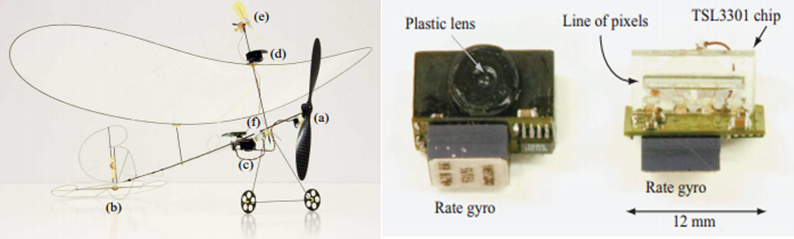
\includegraphics[width=.6\textwidth]{figures/10gr.png}
\caption[Dispositivo volador 10 gramos]{Dispositivo volador que toma imágenes de las murallas para detectar los patrones de textura\\
{\scriptsize (Fuente: \citep{4058367})}}
\label{fig:10gr}
\end{figure}

Estos dispositivos capaces de sobrevolar un recinto pequeño o casas determinan según las texturas de las paredes y su distorsión, la posición relativa dentro del recinto con respecto a la pared fotografiada y utilizando el giroscopio, previenen choques. En la  \autoref{fig:murallas} se observa cómo se generan los patrones de texturas en las murallas para realizar las pruebas.\\

\begin{figure}[ht!]
\centering
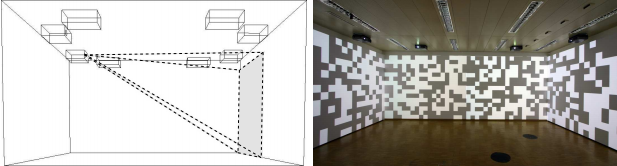
\includegraphics[width=.6\textwidth]{figures/Murallas.png}
\caption[Proyección en murallas vision based]{Proyectores que generan los patrones en las murallas con los cuales los autores realizaron las pruebas\\
{\scriptsize (Fuente: \citep{4058367})}}
\label{fig:murallas}
\end{figure}

Los resultados muestran que la solución es factible, sin embargo no puede controlarse la altitud, y para ello los autores plantean el desarrollo de un \textit{3D visión based tracking system}.

\subsection{Infrarrojo}

La tecnología Infrarroja es una de las más utilizadas para localizar personas y objetos mediante el uso de emisores y receptores infrarrojos.

Una forma posible de utilizar la radiación infrarroja en sistemas de posicionamiento \textit{indoor} es poner en el objeto o persona a localizar, un transmisor infrarrojo con un identificador único. Luego, los receptores son colocados en lugares dentro del recinto, los cuales pueden detectar este identificador único y comunicar a un software especializado, el cual se encarga de calcular la posición mediante la distancia entre el transmisor y receptor. Esta tecnología inalámbrica presenta grandes ventajas. En primer lugar, al no poder atravesar paredes, es fácil confinar las ondas en un recinto. Por otra parte, la radiación infrarroja no se ve afectada por la interferencia electromagnética. A pesar de lo anterior, la tecnología infrarroja presenta dos puntos que lo tornan una opción menos factible. Primero, se ve muy afectado por el efecto de \textit{multipath-propagation}. Además, su implementación requiere hardware y software costoso, por lo que no es tan accesible.

\subsection{Técnicas basadas en Sonido}

La tecnología de ultrasonido utiliza las ondas de ultrasonido para medir la distancia entre una estación base que se encuentra fija, y el objeto a localizar. Para implementar este tipo de sistema, múltiples receptores deben estar sincronizados. Esta sincronización se logra mediante el uso de ondas de radio o radiación infrarroja, ya que estas son mucho más rápidas que las de ultrasonido. El funcionamiento consiste en que los transmisores envían ondas de radio y de ultrasonido al mismo tiempo. Las ondas de radio alcanzan casi instantáneamente a los receptores, con lo cual se pueden sincronizar. Posteriormente cada receptor detecta las ondas de ultrasonido al momento en que arriban, y con esta diferencia de tiempo, es posible calcular la distancia a cada receptor, así se genera una posición relativa dentro de la sala de medición.

Las ventajas de este sistema son los bajos costos de implementación, y la capacidad de funcionar a pesar de la mayoría de las obstrucciones presentes. Las desventajas por su parte son la alta complejidad de desarrollar esta tecnología en sistemas de gran escala, por la sincronización de los receptores. Además la temperatura es uno de los factores más críticos en la velocidad del sonido, es por ello que la gran mayoría de los sistemas basados en ultrasonidos incluyen sensores para compensar estas fluctuaciones de temperatura. Otros factores menos influyentes incluyen la presión del aire, su contenido de dióxido de carbono y la amplitud del sonido.

Otra forma de utilizar el espectro de sonido, y el ultrasonido, es lo que se denomina \textit{acoustic background spectrum}.

En este caso, los autores sugieren una metodología la cual no requiere infraestructura \cite{Tarzia:2011:ILW:1999995.2000011}, es decir las redes inalámbricas son prescindibles. El método consiste en un mapeo \textit{fingerprint} o huella, la cual registra el sonido ambiente de un determinado lugar, y luego construye una base de datos de todas las mediciones realizadas. Posteriormente para estimar la posición del usuario, realiza una comparativa con su actual \textit{fingerprint} y lo contrasta con la base de datos, eligiendo de esta manera la posición más “cercana” según el algoritmo de estimación seleccionado.

El objetivo principal es determinar la posición mediante un dispositivo móvil, como puede ser un Smartphone, de manera rápida y económica a una resolución de una sala de mediano tamaño. La principal ventaja es que no se requiere prácticamente infraestructura por detrás, solo basta los sensores de sonido del equipo móvil.

El principal problema a resolver es entonces traducir los fingerprint a \textit{roomlabels}, es decir la medición actual registrada por el dispositivo móvil, mapearla a una etiqueta de la posición dentro de la sala. Para la realización del fingerprint los autores determinan que este debe ser:

\begin{itemize}
\item Distintivo
\item Responsivo
\item Compacto
\item Eficientemente computable
\item Robusto al ruido
\item Invariante al tiempo
\end{itemize}

Para ello crean \textit{Acoustic background Spectrum} (ABS) que cumple estas condiciones ya que tiene en cuenta ruidos típicos de la vida cotidiana como puede ser sonidos de computadoras, aire acondicionado, entre otros. Para la obtención del \textit{fingerprint} elaboran diversas técnicas basada en el estudio de los sonidos como se aprecia en la  \autoref{fig:abs}.

\begin{figure}[ht!]
\centering
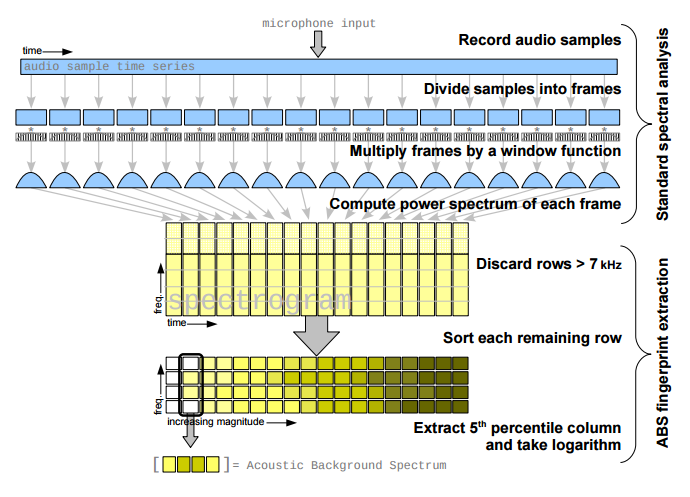
\includegraphics[width=.6\textwidth]{figures/abs.png}
\caption[Método \textit{Acoustic Background Spectrum}]{Descripción del método ABS con el cual se realiza la obtención del mapeo \textit{fingerprint}\\
{\scriptsize (Fuente: \cite{Tarzia:2011:ILW:1999995.2000011})}}
\label{fig:abs}
\end{figure}

Luego de obtener el \textit{fingerprint} los autores usan algoritmos de clasificación, es decir aprendizaje supervisado, como es nearest-neighbor. Se realizaron pruebas en 33 habitaciones distintas, obteniendo una exactitud de 69\%, lo cual muestra resultados aceptables para el posicionamiento utilizando sonidos. Finalmente concluyen que dos \textit{fingerprint} menos exactos pueden ser mejorados si se usan en conjunto, como es el caso de ABS con WiFi.

\subsection{\textit{Wi-Fi}}

\textit{Wireless Local Area Network} (WLAN) puede usarse para estimar la ubicación de un dispositivo móvil dentro de un recinto, dado que la infraestructura WLAN está muy extendida de acuerdo con el aumento de la demanda de redes de comunicaciones, por lo que este enfoque es ampliamente utilizado para posicionamiento \textit{indoor}. Por esta razón, una de las principales ventajas del uso de la técnica de localización Wi-Fi es su rentabilidad ya que no se requiere adicionar infraestructura en lugares donde ya se encuentran estas redes. Otra ventaja de usar WLAN es que no se requiere una línea de visión con los emisores de señales. Es el método más popular que utiliza  \textit{Received Signal Strength Indicator} (RSSI), o intensidad de la señal recibida dentro de las tecnologías inalámbricas y que en este caso son extraídas de las redes IEEE 802.11

En una WLAN, un nodo emite / recibe señales de radiofrecuencia hacia / desde el enrutador inalámbrico, que se puede usar para determinar ubicación precisa de cualquier dispositivo con Wi-Fi habilitado utilizando técnicas que son detalladas posteriormente en esta memoria.

Es la tecnología inalámbrica más utilizada en el mundo, además por seguir un estándar, está claramente definida y sus protocolos funcionan en cualquier parte del mundo. Sus frecuencias son 2.4 GHz y 5 GHz, además es muy escalable utilizando access point, y está muy masificado en dispositivos móviles. Por lo anterior, Wi-Fi se ha vuelto la alternativa más utilizada en técnicas de posicionamiento en interiores.

Recientes investigaciones demuestran que es posible alcanzar una precisión de aproximadamente 3-5 metros \citep{6834746}. Uno de los problemas más grandes son la necesidad de cablear la infraestructura para los routers y el alto consumo de energía que se presenta en ellos. Otro problema presente en la mayoría de las tecnologías inalámbricas es la atenuación de la señal por murallas, objetos o el mismo cuerpo humano.

\subsection{\textit{RFID}}

La tecnología RFID se basa en lectores RFID con una o más antenas, y tags activos o pasivos. Los tags activos poseen una batería, con lo cual son capaces de emitir señales autónomamente, mientras los tag pasivos no poseen batería y requieren de incentivos externos para emitir sus señales. Típicamente se puede poner datos dentro de cada tag, los cuales ayudan a determinar las posiciones. Los datos almacenados dependen estrictamente de la memoria de los tags respectivos.

La localización mediante RFID puede categorizarse en dos tipos, los cuales son localización del lector y localización de tags. En la localización del lector RFID, su precisión depende estrictamente de la densidad de tags dispuestos en el recinto, es decir, la cantidad sobre el área cubierta. Este método funciona de la siguiente manera, el usuario porta un lector y lee los tags dispuestos en distintas posiciones. Cada tag posee información de la posición relativa, con lo cual es fácil reconocer la posición del usuario. Una desventaja obvia, es la poca escalabilidad debido al gran número de tags RFID. 

El segundo método, consiste en determinar la localización del tag RFID. En este caso el usuario no porta un lector, sino que un tag, y los lectores son puestos en lugares estratégicos dentro del recinto, así cuando el usuario transita, los lectores son capaces de determinar en qué lugar fue leído el tag asociado al usuario y determinar su posición. Este método es incluso más costoso que el anterior, ya que los lectores RFID son más caros que los tags. 

Las restricciones más grandes de la tecnología RFID son el corto alcance que este presenta y la posibilidad de leer solo unos pocos tags a la vez. Sin embargo, sus ventajas son muchas, entre ellas se encuentran la alta seguridad de transmisión, alta tasa de transferencia, no requiere línea de visión directa y presenta relativamente bajos costos. 

\subsection{\textit{Bluetooth}}

Bluetooth se ha convertido en el estándar para redes inalámbricas de área personal, WPAN por sus siglas en ingles. Opera en la banda de 2.4 GHz, sin embargo, posee menor alcance que otras tecnologías de radio frecuencia como por ejemplo WLAN, aun a pesar de ello se han registrado implementaciones a gran escala de posicionamiento \textit{indoor} utilizando esta tecnología \citep{BT}. Su rango típicamente alcanza entre 10 a 15 metros, ya que es pensado principalmente para comunicaciones directas entre emisor y receptor dentro de un rango corto, como puede ser una casa o una sala de mediano tamaño. A pesar de esto, el creciente interés de múltiples aplicaciones ha vuelto a la tecnología Bluetooth muy relevante, ya que hoy en día está presente en smartphones, computadores, notebooks entre otros. Con esto presente, no se requiere adicionar mayor hardware a los teléfonos celulares para implementar un sistema de localización, ya que prácticamente todos estos dispositivos cuentan con la tecnología Bluetooth integrada.

Bluetooth es una tecnología de bajo consumo energético y bajo costo, por lo que es eficiente y factible en el desarrollo de sistemas de localización \textit{indoor}. Los tags bluetooth son pequeños y por esta razón pueden ser colocados en múltiples lugares para asegurar la cobertura de una región. Los tags poseen un ID único como puede ser la MAC u otro identificador generado por el fabricante.

En los últimos años, nuevos dispositivos han sido creados con el objetivo de ayudar al crecimiento del Internet de las cosas. Estos dispositivos son conocidos como Bluetooth beacons y muchas empresas han creado su propio hardware, además proveen kits de desarrollo de software para hacer más fácil la integración de esta tecnología en sistemas. Empresas como Apple, Kontakt.io, Estimote, entre otras, venden estos tags sin ninguna restricción en cuanto a su uso, por lo que existen múltiples casos de uso como se puede ver en \citep{kontaktio}.

\subsection{Otras tecnologías}

Existen muchas otras tecnologías, que en este momento son menos relevantes pero que sin embargo son investigadas frecuentemente para crear nuevos sistemas de posicionamiento o para mejorar y complementar los existentes. Entre las más relevantes se puede destacar ZigBee, \textit{Ultra Wide Band} (UWB), GSM, radio FM y sensores inerciales de los dispositivos móviles.

La localización en interiores utilizando \textbf{ZigBee} se basa en la creación de una red de sensores con posiciones conocidas, y un sensor ZigBee denominado \textit{target} del cual se desea conocer su posición. Ya que estos nodos sensores pueden comunicarse entre sí, la fuerza de la señal recibida por los sensores es comúnmente usada para localizar al \textit{target}. Se han utilizado múltiples algoritmos de localización con resultados favorables dependiendo del ambiente como se puede observar en \citep{6156509}.

\textbf{UWB} usa un pulso de radio de un sub-nanosegundo para transmitir datos en un amplio ancho de banda. Por estas características, se considera que no interfiere en otras señales de radio, por lo tanto, puede utilizarse en cualquier espectro de emisión.  Utiliza bajo consumo de energía, y además en teoría no es afectado por \textit{multi-path propagation}, es decir, la interferencia que se produce en las señales al rebotar o reflectarse en ciertas superficies.

Las ondas de radio \textbf{FM} son utilizadas ya que pueden eventualmente evitar algunas complicaciones presentes en otras tecnologías inalámbricas como Wi-Fi utilizando los mismos algoritmos.

\textbf{GSM} es utilizado principalmente en redes celulares, y cubre diferentes tipos de frecuencias, además está en prácticamente todos los edificios y ciudades, con lo cual no requiere mayor infraestructura. A diferencia de FM tiene menor distancia de propagación, por lo cual si sirve en interiores. El principal problema es que GSM está fuertemente patentado y es complejo realizar ensayos y pruebas sobre él.

Finalmente, los sensores inerciales se refieren a sensores que ocupan la inercia para medir aceleración como puede ser giroscopio, acelerómetro. En este contexto, los sistemas de posicionamiento basado en sensores son sistemas que explotan los sensores de movimiento y rotación, para continuamente calcular la posición, velocidad y orientación sin la necesidad de utilizar hardware o referencias externas.

La gran parte de los equipos móviles actuales cuenta con acelerómetro y brújula, con lo cual se puede realizar una navegación estimando ciertos parámetros. En \citep{6071934, 5766963} , los autores plantean un modelo basado en los sensores de los dispositivos, ya que al ser capaces de detectar los pasos, se puede establecer una ruta predefinida dentro de un determinado lugar, pero la única desventaja es que es el usuario quien debe decirle al dispositivo la posición inicial o algún punto de referencia.

Los autores generan sus mapas con OpenStreetMap, luego realizan un algoritmo llamado \textit{First Fit}, para detectar la dirección del movimiento y realizar el \textit{matching} con la ruta predefinida, con ello se puede determinar la posición relativa del usuario al lugar en donde comenzó. La \autoref{fig:acel} muestra esta situación.

\begin{figure}[ht!]
\centering
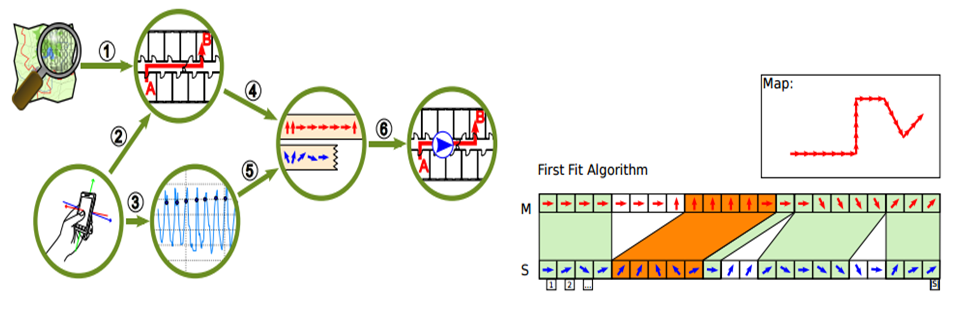
\includegraphics[width=.6\textwidth]{figures/acel.png}
\caption[Navegación mediante sensores inerciales \textit{First Fit} ]{\textbf{(a)} A la izquierda, proceso completo para la navegación utilizando acelerómetro y conteo de pasos. \textbf{(b)} A la derecha, método First-Fit para anticipar y predecir posición del usuario.\\
{\scriptsize (Fuente: \citep{6071934, 5766963})}}
\label{fig:acel}
\end{figure}

\textit{First Fit} realiza una especie de \textit{lookahead} para establecer el match con los pasos de la ruta y si los pasos que está detectando actualmente son errores. Con esto, puede mirar los pasos futuros y aproximar en donde se encuentra el usuario.

Los autores evalúan su propuesta en tres distintos escenarios, primero en exteriores para medir exactitud, luego en interiores para establecer si la solución es robusta, y luego en un escenario relativamente grande pero que es \textit{indoor}. Los autores concluyen que la solución es factible para la navegación, pero no para el posicionamiento, ya que es el usuario quien ingresa su posición estimada según ciertos nodos dentro del edificio. El sistema es escalable, pero requiere realizar las rutas predefinidas, lo cual puede ser mucho trabajo en edificaciones demasiado grandes.

\subsection{Comparativa de tecnologías \textit{Wireless}}

Dado que los mejores resultados presentes en la literatura corresponden a las tecnologías \textit{Wireless}, ya sean de sonido, radiofrecuencia, entre otros, a continuación, se muestran las ventajas y desventajas de cada una de ellas.

\begin{table}[!ht]
\centering
\caption[Comparativa Tecnologías Inalámbricas]{Tabla comparativa tecnologías inalámbricas}
\label{my-label}
\begin{tabular}{|c|c|c|c|c|c|}
\hline
            & Precisión {[}m{]}             & Rango {[}m{]} & Costo & Complejidad & Ambiente       \\ \hline
Infrarrojo  & \(10^{-2}\) - 1 & 1-5           & Alto  & Baja        & Indoor         \\ \hline
Ultrasonido & \(10^{-2}\)     & 2-10          & Medio & Baja        & Indoor         \\ \hline
Wi-Fi       & 1-10                          & 20-50         & Medio & Baja        & Indoor/Outdoor \\ \hline
RFID        & \(10^{-1}\)-1   & 1-10          & Bajo  & Baja        & Indoor         \\ \hline
Bluetooth   & 1-10                          & 1-30          & Bajo  & Baja        & Indoor/Outdoor \\ \hline
\end{tabular}
\end{table}

Ninguna tecnología presentada anteriormente es completamente efectiva en todos los escenarios, por lo que la elección de estas se debe hacer según las características del lugar, como su dinámica de cambio, obstáculos presentes, tamaño, entre otros. En la \autoref{fig:comparativa} se resume el alcance y características de cada tecnología de posicionamiento.


\begin{figure}[!ht]
\centering
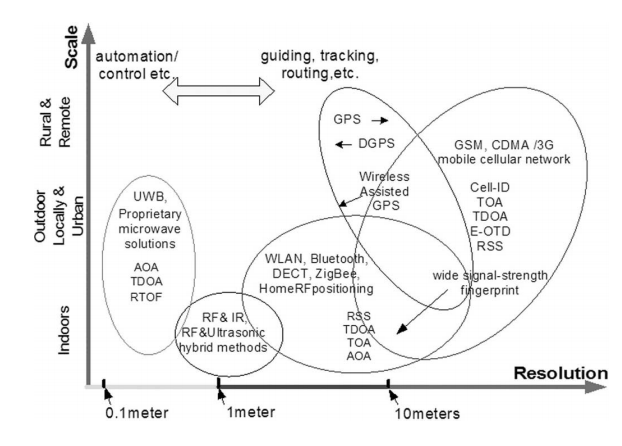
\includegraphics[width=.6\textwidth]{figures/comparativa.png}
\caption[Comparativa tecnologías inalámbricas]{Comparativa de distintas tecnologías inalámbricas basado en su resolución y alcance.\\
{\scriptsize (Fuente: \citep{Liu:2007:SWI:2220431.2221077})}}
\label{fig:comparativa}
\end{figure}


\section{Técnicas  matemáticas Wireless para localización indoor}

No es sencillo determinar un modelo completo para la propagación de ondas en interiores debido a muchos problemas que se presentan como lo es multipath, baja probabilidad de la línea de visión (LOS), y otros factores determinantes como tipo de material del edificio, superficies que reflejan ondas, el mismo cuerpo humano y objetos en movimiento. Por lo mismo es necesario establecer modelos matemáticos que reduzcan el error generado por la influencia de los factores antes mencionados.\\

Habitualmente se categorizan las técnicas matemáticas para la localización en interiores en 3 grandes grupos: Proximidad, Triangulación y \textit{fingerprint} (\textit{scene analysis}).

\subsection{Proximidad}

Es el método más simple, y se basa en determinar una posición simbólica y aproximada de la posición del usuario. Para lograrlo, existe una grilla de antenas o emisores de ondas de radio, y según la señal más fuerte detectada por el usuario, es donde se localiza en el sistema. Este tipo de localización es ampliamente usado en redes celulares, ya que permite determinar la posición de un dispositivo con una precisión de 50-200 m, sin embargo, no es buena en espacios reducidos. Por lo mismo se dice que este método tiene una alta varianza, y muchas veces no satisface la necesidad de localización. La ventaja es que al ser simple puede utilizarse en la mayoría de las redes inalámbricas, como lo es infrarrojo, RFID, Cell-ID, GSM.

Por lo anterior, habitualmente se dice que esta técnica es para saber en qué espacio geográfico o región está el usuario, no para saber su posición exacta \citep{Liu:2007:SWI:2220431.2221077}.

\subsection{Triangulación}

La triangulación utiliza las propiedades geométricas de un triángulo para estimar la posición del objeto.  La triangulación se divide en 2 puntos: lateración y angulación. Por una parte, la lateración estima la posición midiendo las distancias hacia múltiples puntos de referencia también llamados beacons. Angulación por su parte, no utiliza las distancias, sino que los ángulos relativos a cada beacon o punto de referencia. La  \autoref{fig:triangulacion} muestra cómo se calculan las posiciones relativas con lateración y angulación.

\begin{figure}[ht!]
\centering
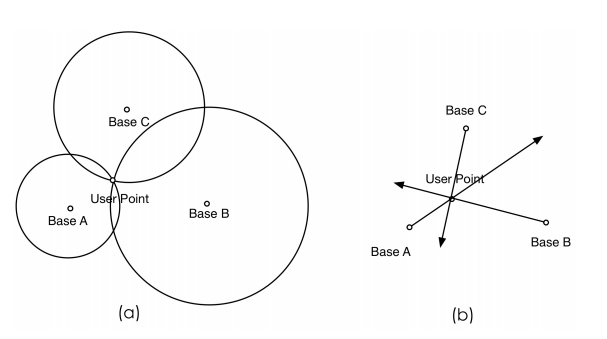
\includegraphics[width=.6\textwidth]{figures/triangulacion.png}
\caption[Lateración y Angulación]{Técnicas de triangulación basadas en lateración \textbf{(a)} y angulación \textbf{(b)}\\
{\scriptsize (Fuente: \citep{Liu:2007:SWI:2220431.2221077})}}
\label{fig:triangulacion}
\end{figure}

Si se conoce las \textit{base station} emisoras de ondas, lateración puede calcular la posición basado en un modelo matemático en donde se utiliza la intersección de tres círculos. Por otra parte, angulación utiliza la información del ángulo de llegada de las señales y con esto puede trazar 3 vectores, en donde la intersección representa la posición del objeto receptor.

El principal problema es establecer la distancia para lateración, y los ángulos para angulación. Para ello se han diseñado muchos acercamientos que permiten obtener esos valores.

\begin{enumerate}
\item \textbf{Técnicas de lateración }
\begin{enumerate}
\item \textbf{ToA (Time of arrival):} En ToA, la distancia del objeto móvil hacia las estaciones es directamente proporcional al tiempo de propagación, y además se sabe la velocidad de propagación de las ondas, que habitualmente es la velocidad de la luz siempre y cuando se transmitan en el aire. El dispositivo del usuario envía paquetes con las marcas temporales, es decir la hora en que se envía el paquete, luego la estación beacon puede determinar la hora en que llega el paquete, y haciendo la diferencia se obtiene el tiempo de propagación. ToA presenta dos grandes problemas, uno es que todos los dispositivos deben estar altamente sincronizados, y segundo, es que los paquetes deben estar etiquetados con información de tiempo de envió \citep{102710}.

\item \textbf{TDoA (Time difference of arrive):} Es similar a ToA, sin embargo en este caso no se necesita el tiempo de emisión del transmisor, solo se requiere el tiempo de llegada a cada uno de las estaciones base o beacons y mediante la diferencia de tiempo entre ellas establecer la posición. Para lograrlo, cada TDoA, se representa como una curva hiperbólica de las potenciales posiciones asumiendo distintos tiempos de transmisión como se muestra en la \autoref{fig:tdoa} . Donde se intersectan las curvas de a lo menos 2 estaciones beacons, es donde se transmitió la señal, por lo mismo es la posición del usuario.

\begin{figure}[ht!]
\centering
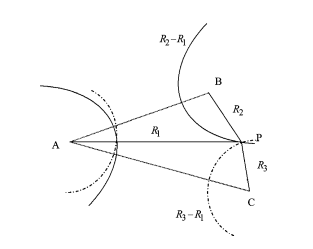
\includegraphics[width=.6\textwidth]{figures/tdoa.png}
\caption[Curvas Hiperbólicas TDoA]{Curvas hiperbólicas de TDoA que estiman la posición basado en el tiempo de transmisión.\\
{\scriptsize (Fuente: \citep{Liu:2007:SWI:2220431.2221077})}}
\label{fig:tdoa}
\end{figure}

Habitualmente por la complejidad del método, se utilizan linealización de las fórmulas del hiperboloide, a través de expansión en series de Taylor para luego crear algoritmos iterativos computacionalmente eficientes como se muestra en \citep{4103919}.

\item \textbf{Método basado en RSS (Received signal strength):}  Los métodos anteriores tienen algunos inconvenientes, primero, es complejo encontrar una línea de visión entre el emisor y receptor, además de la propagación por ondas de radio que puede presentar efectos de multicaminos, es decir, una misma onda llega al receptor por dos vías distintas, debido a la reflexión u otros factores. Una alternativa es estimar la distancia utilizando la atenuación de la fuerza la señal.

Existen modelos teóricos y empíricos, los cuales intentar predecir la distancia utilizando la diferencia entre la fuerza de la señal entre el transmisor y el receptor. Este método no es muy utilizado, debido al desvanecimiento de las señales en interiores, sin embargo puede utilizarse usando algunos pre procesamientos o mejoras, como por ejemplo establecer contornos predefinidos de señales RSS en forma de elipses como muestran los autores en \citep{1423549}.

\end{enumerate}

\item \textbf{Técnicas de angulación }
\begin{enumerate}
\item \textbf{AoA ( Angle of arrival):} Como se define en \citep{665} , la localización del objetivo puede realizarse mediante la intersección de múltiples líneas con una dirección dada por el ángulo entre cada estación y el receptor. Los métodos AoA deben utilizar al menos dos puntos de referencia o estaciones beacon,  y los dos ángulos respectivos con respecto al objeto que se quiere realizar la localización. La principal ventaja es que requiere tantas estaciones como el número de dimensiones en donde se requiere localizar el objeto, por ejemplo si se necesita determinar la posición en tres dimensiones, se requieren tres estaciones bases. Además, no se necesita sincronización de tiempos.

Por otra parte, es complejo y difícil de implementar, además de requerir software especializado, ya que para una localización muy precisa el ángulo debe ser medido con muy poco error y esto es difícil de lograr. Al igual que otras técnicas se ve afectado por propagación \textit{multipath} y desvanecimiento de las señales, interferencia y por la dirección de la apertura de medición. La \autoref{fig:angulacion} muestra el comportamiento de AoA.

\begin{figure}[ht!]
\centering
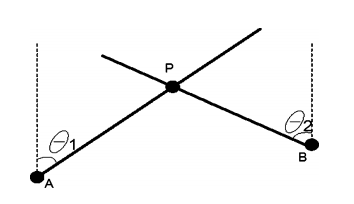
\includegraphics[width=.6\textwidth]{figures/angulacion.png}
\caption[Proyección de vectores AoA]{Proyección de vectores basado en ángulo de incidencia de las ondas sobre el objeto o dispositivo móvil.\\
{\scriptsize (Fuente: \citep{Liu:2007:SWI:2220431.2221077})}}
\label{fig:angulacion}
\end{figure}

\end{enumerate}
\end{enumerate}


\subsection{Fingerprint}

Se denomina \textit{fingerprint} o \textit{scene analysis} al tipo de algoritmos que en primer lugar recolecta características de un lugar y luego estima la localización en tiempo real utilizando las características, contrastándolas con las características actuales. Lo más habitual es utilizar Fingerprint basado en RSS.

Fingerprint presenta dos etapas, la etapa offline y la etapa online. Durante la etapa offline se realiza un reconocimiento de las características del lugar, en donde se mide las coordenadas de cada estación base y la fuerza de la señal en determinados lugares, obteniendo así un mapa de señales del entorno.  Durante la etapa online se utiliza la señal actual recibida de cada estación base y un modelo generado en la etapa offline, generando así una estimación de la posición del usuario. La  \autoref{fig:finger} muestra el funcionamiento a nivel general de Fingerprint:

\begin{figure}[ht!]
\centering
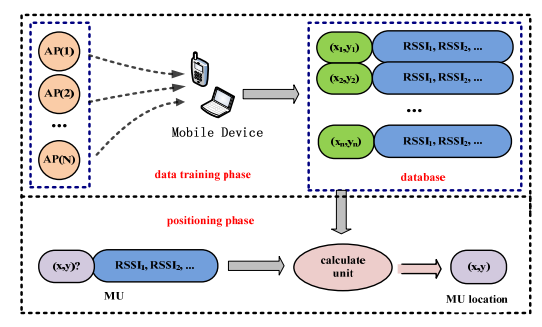
\includegraphics[width=.6\textwidth]{figures/finger.png}
\caption[Proceso de creación Fingerprint]{Proceso de captura de características Fingerprint y elaboración del modelo para estimar la posición.\\
{\scriptsize (Fuente: \citep{Liu:2007:SWI:2220431.2221077})}}
\label{fig:finger}
\end{figure}

Fingerprint se divide en dos grandes aristas, \textit{map-based Fingerprint} y \textit{map-free} Fingerprint:

\begin{enumerate}
\item \textbf{Map-based Fingerprint}

Este caso utiliza la etapa offline y online, en donde en la etapa offline se generan los radio-map de cada posición, es decir, asociar una característica de las señales según la posición geográfica en donde se toma la medición. Existen dos tipos de radio-map, los cuales son radio-map de tipo valor medio, y radio-map de tipo función de densidad de probabilidad. En el radio-map de tipo valor medio existe un número limitado de puntos en donde se toman las mediciones de las señales, mientras que el radio-map de tipo función de densidad de probabilidad, puede representar todos los puntos del lugar como una función continua. Para la estimación de la posición se han realizado variados acercamientos como es modelos de probabilidad, kNN, redes neuronales, SVM, estimación de máxima verosimilitud, estimación bayesiana \citep{Liu:2007:SWI:2220431.2221077, 1192765}.

Para la generación de los radio-maps se utiliza habitualmente tres técnicas, las cuales son \textit{Model Based Estimation}, Medición Offline y calibración Online. \textit{Model Based Estimation} no confía plenamente en las señales RSS, si no que utiliza distintos modelos de propagación como son \textit{Wall attenuation factor} \citep{Bahl00radar:an} , 2D-ray tracing y otros modelos de propagación de las señales para estimar la fuerza de la señal en determinados puntos del espacio y generar el radio-map. La siguiente ecuación describe la fórmula de la atenuación de señales por el efecto de las paredes.

\begin{equation}
P(d)[dBm] = P(d_{0})[dBm] - 10nlog (\frac{d}{d_{0}}) - \left\{ \begin{array}{lcc}
             nW*WAF &   si  & nW < C \\
             \\ C*WAF &  si & nW \geq C \\
             \end{array} \right.
\end{equation}

   

En donde \(n\) representa la velocidad con la que aumenta la pérdida de poder de la señal con la distancia. \(P(d_{0})\) es el poder de la señal en cierto punto de referencia \(d_{0}\) y \(d\) es la distancia que separa al transmisor y receptor. \(C\) es el máximo número de paredes para el cual el factor de atenuación hace alguna diferencia. \(nW\) es el número de paredes y \(WAF\) es el factor de atenuación por las paredes. Habitualmente \(n\) y \(WAF\) se conocen, ya que depende del lugar y orden de los objetos dentro de un edificio.

Por otra parte, se tiene mediciones offline, en donde se realiza un proceso lento y tedioso, de medir cada punto del lugar en donde se realiza la localización. Mientras más puntos se registran, mejor será el radio-map ya que tiene un mayor número de datos de entrenamiento. Para reducir el trabajo, algunos autores han utilizado robots para registrar la medición de las señales \citep{5398451}. La \autoref{fig:robots} muestra cómo se utiliza un robot para tomar mediciones de las señales en determinados puntos, en este caso los beacons corresponden a tags RFID.

\begin{figure}[ht!]
\centering
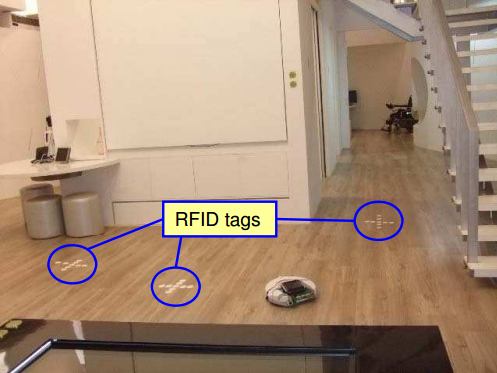
\includegraphics[width=.4\textwidth]{figures/robots.png}
\caption[Robots para map Fingerprint]{Robot que toma automáticamente las características para elaborar el mapeo fingerprint de un determinado lugar.\\
{\scriptsize (Fuente: \citep{Liu:2007:SWI:2220431.2221077})}}
\label{fig:robots}
\end{figure}

Por último, calibración online tiene en cuenta que se requiere mucho esfuerzo para realizar las mediciones y obtener las características de señales, además si el entorno cambia constantemente es probable que las señales también cambien y todo el registro se pierda y deba ser realizado nuevamente. Entonces calibración online combina las dos técnicas anteriores, dejando ciertos nodos ancla que miden constantemente la señal en esos puntos, y mediante \textit{model based estimation}, pueden estimar la fuerza de la señal en otros lugares en donde no hay nodos ancla. Los nodos ancla pueden realizar mediciones cada cualquier intervalo de tiempo, ajustando el modelo, y por lo mismo no se ve afectado por cambios en el entorno.

\item \textbf{Map-Free Fingerprint} 

Map-based fingerprint puede utilizarse con cualquier red inalámbrica o incluso otros tipos de Fingerprint, como ultrasonido, campos magnéticos, entre otros. Sin embargo la complejidad para registrar mediciones aumenta cuando el área a mapear aumenta, además la mantención temporal del radio-map es un proceso engorroso y lento. Map-free reduce esta complejidad, utilizando otras formas de localizar usando fingerprints.

En \cite{Wang:2012:NNW:2307636.2307655} el autor observa patrones de las señales en ciertos lugares como el ascensor o el pasillo, y con estos puntos de referencia utiliza aprendizaje no supervisado para estimar la posición del usuario. Combinando esta información junto con los acelerómetros y sensores del dispositivo móvil, el autor muestra cómo puede obtener una posición estimada muy cercana a la real. Entonces este tipo de Fingerprint, se basa en el patrón del punto de referencia actual y las mediciones de puntos de referencia anteriores. Por lo mismo se dice que este método no soporta localización estática.

\end{enumerate}

\subsubsection{Formulación del problema Fingerprint}

En la técnica de \textit{Fingerprint} el área es dividida en un conjunto de puntos de referencia (RPs), \(P = \{p_{j} = (x_{j}, y_{j}) \ | \ j = 1,...,N\}\) en donde \(P\) define el conjunto cartesiano de RPs, que no necesariamente son un conjunto de puntos equidistantes entre si \citep{7874080}. El dispositivo móvil graba un conjunto de mediciones \textit{Fingerprint} RSS en los instantes \(t_{m} ,\ m = 1,...,M\) con magnitudes RSS \( \ r_{j}^{i}(t_{1}),..., r_{j}^{i}(t_{M}) \ \) en cada RP, donde \(i\) indica el índice del access point desde el conjunto de access points \( \mathcal{L} = \quad \{AP^{1}, ..., AP^{L}\}\). Generalmente se toma el mismo número de ejemplos de entrenamiento, \(M\) en cada RP. Los Fingerprints RSS de todos los access point en el tiempo \(t_{m}\) en el punto \(p_{j}\) están organizados en un vector \(r_{j}(t_{m}) = [(r_{j}^{1}(t_{m}),...,(r_{j}^{L}(t_{m})]^{T}\). El radio map completo guardado en el instante \(t_m\) puede ser reconocido por la siguiente matriz:


\begin{align}
\def\arraystretch{2.2}
   R(t_{m}) = (\textbf{r}_{1}(t_{m}), ..., \textbf{r}_{N}(t_{m})) = 
  \left[ {\begin{array}{cccc}
   r_{1}^{1}(t_{m}) & r_{2}^{1}(t_{m}) & ... & r_{N}^{1}(t_{m}) \\
   r_{1}^{2}(t_{m}) & r_{2}^{2}(t_{m}) & ... & r_{N}^{2}(t_{m}) \\
   r_{1}^{3}(t_{m}) & r_{2}^{3}(t_{m}) & ... & r_{N}^{3}(t_{m}) \\
   r_{1}^{4}(t_{m}) & r_{2}^{4}(t_{m}) & ... & r_{N}^{4}(t_{m}) \\
  \end{array} } \right] \ , \quad 
m\ = \ 1,...,M.
\end{align}
 

Un subconjunto de RPs con el mayor grado de similaridad es denotado como \(\mathcal{K}\) y está definido como \(\mathcal{|K|} = K\). Esta similaridad es definida por cada método y es detallada posteriormente.

En la fase online el usuario recibe una medición RSS \quad \(\textbf{y} = (y^{1}, ..., y^{M}) ^{T}\). Entonces el objetivo es simple; encontrar la localización \(\hat{\textbf{p}} = ( \hat{x}, \hat{y})\), basado en una regla que compara la medición online contra el radio map de \textit{fingerprints} como: 

\begin{equation}
\hat{\textbf{p}} = f(\textbf{R}, \textbf{y})
\end{equation}

En donde \(R\) denota la colección de radiomaps en todas las instancias guardadas. A continuación, se muestran los tres acercamientos principales para la localización utilizando Fingerprint.

\subsubsection{Acercamientos convencionales de Fingerprint}

\begin{enumerate}
\item \textbf{Acercamiento determinista:} En esta forma de resolver el problema de Fingerprint, la posición que logra la mayor similaridad con la posición real es alcanzada utilizando la siguiente formulación:

\begin{equation}
\hat{\textbf{p}} = \underset{j=1,...,N}{\mathrm{argmin}} \quad d( \breve{\textbf{r}}_{j}, \textbf{y})
\end{equation}

En donde \(\breve{\textbf{r}}\) es el valor representativo del Fingerprint en el \(j-esimo\) RP \citep{832252} y \(d( \breve{\textbf{r}}_{j}, \textbf{y}) \) define una medida de distancia típica \citep{6817920}. En el caso de promedio de tiempo, el valor representativo es el promedio de los Fingerprints durante el tiempo en que fueron medidos. La distancia Euclidiana también puede ser utilizada, definida como: 

\begin{equation}
d( \breve{\textbf{r}}_{j}, \textbf{y}) = \lVert y - \breve{\textbf{r}}_{j} \rVert_{2} \quad j = 1,..., N.
\end{equation}
   

Ya que el número de access point disponibles  varia en la superficie a localizar, la posición es típicamente estimada sobre los AP visibles y los AP desconocidos se estiman en un valor que indica una señal débil o un valor imposible de obtener (100 dBm).

\item \textbf{Acercamiento probabilista:} En este acercamiento, una sola medida RSS puede ser no suficiente para estimar la posición, ya que no representa la variación temporal de los datos en la propagación en interiores. El desempeño del acercamiento determinista puede ser mejorado si en vez de utilizar solo un subconjunto de Fingerprints RSS, todos los Fingerprints son utilizados. En esta presunción se basa el acercamiento estadístico, utilizar todos los Fingerprints para describir de mejor manera el área en cuestión.

La forma en que el acercamiento estadístico estima la posición, se basa en la estimación de Máximo a Posteriori ( MAP) \citep{4907834}, de esta manera MAP estima la posición del usuario maximizando la probabilidad condicional de la posición dado la medición recibida en la etapa online:

\begin{equation}
\hat{\textbf{p}} = \underset{j=1,...,N}{\mathrm{argmax}} \quad f( \textbf{p}_{j} \vert \textbf{y})
\end{equation}

 En donde \( f( \textbf{p}_{j} \vert \textbf{y}) \) es la probabilidad condicional de que el usuario este en \(\textbf{p}_{j}\) dado que recibió el vector \( y \) en la etapa online.
 
Gracias al teorema de Bayes esto puede ser re formulado de la siguiente manera:

\begin{equation} \label{eq:1}
 f( \textbf{p}_{j} \vert \textbf{y}) = \frac{f( \textbf{p}_{j} , \textbf{y})}{f(y)} = \frac{f( \textbf{y} \vert \textbf{p}_{j}) f(\textbf{p}_{j})} {\sum_{j=1}^{N} f( \textbf{y} \vert \textbf{p}_{j}) f(\textbf{p}_{j})} \quad j = 1, ..., N 
\end{equation}

La probabilidad \(f(\textbf{p}_{j})\) es la distribución de la posición del usuario sobre el área completa, y se asume generalmente uniforme ya que no existe conocimiento previo en la posición del usuario, por lo que todos los puntos estudiados son equiprobables. Por lo anterior, \(f(\textbf{p}_{j})\) puede ser ignorado en el problema de maximización, de esta forma el denominador en la ecuación \ref{eq:1} es el mismo para todo \( j= 1, ..., N\) de esta manera, el problema MAP es transformado a :

\begin{equation}
\hat{\textbf{p}} = \underset{j=1,...,N}{\mathrm{argmax}} \quad f( \textbf{y}  \vert \textbf{p}_{j})
\end{equation}


Conocido comúnmente como el estimador de máxima verosimilitud o \textit{Maximum Likelihood (ML)}. 

Lo anterior revela que el acercamiento determinista confía en estimar la densidad a priori \(f( \textbf{y} \ \vert \ \textbf{p}_{j})\). Existen dos formas utilizadas en la estimación de esta distribución de densidad de probabilidad, las cuales son denominadas paramétrica y no paramétrica. La estimación paramétrica trata a la distribución de probabilidad como una distribución analítica conocida, por ejemplo una distribución Gaussiana \citep{Haeberlen:2004:PRL:1023720.1023728} para aproximar las características temporales de las señales RSS. Este enfoque ha sido cuestionado en múltiples investigaciones, debido a lo poco realista que se torna este supuesto en muchos lugares y recintos experimentales. Los primeros acercamientos utilizaban una aproximación log-normal para la distribución, sin embargo, es sesgada y estacionaria sobre pequeños intervalos de tiempo.  Las aproximaciones modernas de estimación paramétrica utilizan funciones Kernel para lograr mejores resultados. 

La estimación no paramétrica no asume nada con respecto a la distribución de Fingerprint RSS. En vez de esto, la distribución es generada utilizando un histograma que cuadra con el radio map construido \citep{Haeberlen:2004:PRL:1023720.1023728, Ladd:2002:RLS:570645.570674}. En este emparejamiento, todos los datos son cuantizados en múltiples niveles y la frecuencia de cada barra del histograma es calculada, para la estimación de \(f( \textbf{y} \ \vert \ \textbf{p}_{j} ) \). El histograma consiste entonces en la concatenación de todas estas barras. Sin embargo, un gran número de ejemplos son necesarios en diferentes instantes de tiempo en cada RP para generar el histograma, lo que es complejo de obtener en la práctica.

\item \textbf{Técnicas de reconocimiento de patrones:} La idea básica de reconocimiento de patrones se basa en clasificadores, que son utilizados con los Fingerprints recolectados y luego son capaces de discriminar una nueva medición RSS desconocida durante la fase online. En la fase de entrenamiento de cada clasificador, el sistema ajusta los parámetros del modelo, mediante el uso del radio map de Fingerprints recolectados en forma de base de datos. En la fase de testing, los datos RSS recibidos desde una posición desconocida son analizados por el clasificador para estimar la posición más cercana. La diferencia entre los algoritmos de reconocimiento de patrones, son en la manera en que utilizan técnicas para emparejar los datos. La salida de estos algoritmos es generalmente un conjunto de probabilidades o verosimilitud de muchas posiciones, con lo cual es posible estimar un centroide de todas las posiciones como solución, o simplemente elegir el que posea la mayor probabilidad.
\end{enumerate}

\subsubsection{Avances recientes en Fingerprint}

La presente sección pretende mostrar los últimos avances en las técnicas de Fingerprint con el objetivo de esclarecer las ventajas y desventajas de estos. Antes, la \autoref{fig:fingerprint_basic} presenta un diagrama de cómo funciona Fingerprint en su forma general:

\begin{figure}[ht!]
\centering
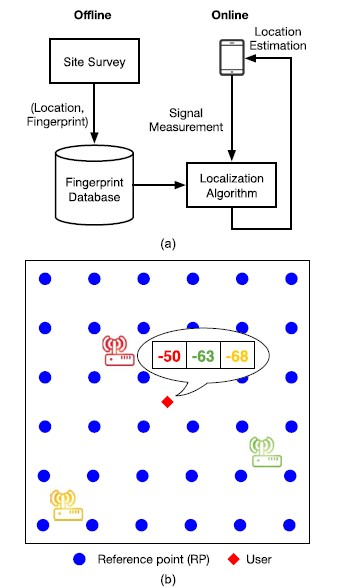
\includegraphics[width=.3\textwidth]{figures/fingerprint_basic.jpg}
\caption[Fingerprint esquema básico]{(a) Flujo básico de fingerprint. (b) radio-map de un sistema de localización indoor\\
{\scriptsize (Fuente: \citep{7174948})}}
\label{fig:fingerprint_basic}
\end{figure}

\begin{enumerate}
\item \textbf{Explotando patrones temporales y espaciales:} El Fingerprint tradicional se basa en la medición de vectores RSS. Debido al ruido en las mediciones, el objetivo puede ser \textit{mapeado} a una posición distinta de vectores de señales similares \citep{6681592}. La precisión puede ser aumentada si son considerados patrones espaciales y temporales, característicos del lugar en el cual se está experimentando.

\begin{itemize}
\item \textbf{Patrones temporales} Son patrones de señales que son encontrados a medida que se camina por el área en donde se desea posicionar. Estos patrones pueden ayudar a mejorar la localización en interiores. Luego, cuando un vector de señales es comparado en una posición fija, los patrones contienen información temporal que pueden ser utilizados para restringir y corregir las señales RSS para la localización base.

\item \textbf{Patrones espaciales} Están caracterizados por asociar señales RSSI con su correspondiente distribución geográfica. Mientras que los patrones temporales requieren conocer el movimiento del usuario, el cual puede ser no determinado o poco preciso en casos reales. Los patrones geográficos de señales pueden ser utilizados para restringir la posición del usuario. Estos patrones incluyen orden de los vectores RRSI, puntos de control en las señales, y la cobertura de las señales dadas por los APs.

\end{itemize}

\item \textbf{Localización colaborativa entre móviles} Muchos de los avances se enfocan principalmente en determinar la posición de un usuario independientemente de los demás dispositivos, sin considerar sus posiciones relativas. Debido a los errores de cada móvil independiente, dos objetivos físicos cercanos pueden ser marcados en diferentes posiciones estimadas. Entonces, si la información de la posición relativa puede ser accedida y utilizada, los resultados en la estimación pueden ser mejorados para la localización individual de cada móvil. Trabajos recientes han desarrollado la localización colaborativa. Estas aristas nacen básicamente de las siguientes tendencias en computación móvil:

\begin{itemize}
\item \textbf{Contexto de localización de interacción social:} En la localización indoor, la gente puede estar cercana en escenarios sociales típicos \citep{Chan2006}. En museos, por ejemplo, la gente busca dentro junto a su familia o amigos. La interacción entre este conjunto determina un patrón de localización.

\item \textbf{Dispositivos móviles penetrantes y sensores avanzados:} En estos días, los \textit{smartphones} han desarrollado muchos sensores, los cuales pueden detectar otros móviles en su vecindario cercano, basado en uno o varios protocolos, como puede ser Bluetooth, WiFi direct, NFC y ondas de sonido. El aumento de los dispositivos móviles con estos sensores provee la posibilidad de mejorar significativamente esta técnica en posteriores investigaciones.
\end{itemize}


\item \textbf{Localización asistida por movimiento: } La localización asistida por movimiento es una de las técnicas híbridas más utilizadas en estos días, debido a la gran penetración en el mercado de dispositivos que presentan sensores en el ámbito móvil. Los más grandes avances consisten en las siguientes dos técnicas:

\begin{itemize}
\item \textbf{Avances en la medición de movimiento:} El monitoreo del comportamiento de una caminata es importante para la localización asistida en movimiento precisa. El mayor desafió en obtener información del movimiento es que los sensores inerciales de los dispositivos móviles sufren de calibración imperfecta y mediciones con ruido. \textit{Step counting} es el mayor acercamiento para capturar el movimiento y dirección de una caminata \citep{6407455}. Trabajos recientes apuntan a mejorar la dirección de la caminata, conteo de pasos y longitud de pasos. Sin embargo, como adaptar estos parámetros a cada usuario, es decir, sus propios perfiles de movimiento es un área desafiante que continua en investigación.

\item \textbf{Modelos de fusión avanzados y eficientes:} Como fusionar el movimiento con y la detección de señales RSS es esencial para mejorar la precisión en la localización en interiores. El modelo usado en fusión necesita capturar la correlación (ya sea temporal o espacial) entre las señales medidas. Sin embargo, si el modelo es altamente complejo, el alto costo computacional también afecta la calidad de la estimación en la localización. A pesar de esto, buscar un algoritmo de fusión eficiente y preciso se ha convertido recientemente en una importante tendencia para la localización asistida por movimiento \citep{6846747}.

\end{itemize}
\end{enumerate}

\chapter{Propuesta de solución}

La propuesta detallada a continuacion tiene como consideracion los siguientes objetivos referentes a este trabajo:

\begin{itemize}
\item Establecer un marco de trabajo para la recolección, entrenamiento y clasificación de algoritmos de machine learning utilizando Bluetooth Lo Energy

\item Comparación de diferentes clasificadores, para determinar sus ventajas y cuales se comportan de mejor forma en la fase de entrenamiento y test, para asi seleccionar los mejores.

\item Utilizar técnicas de reducción de dimensionalidad para reducir la complejidad del problema, y optimizar los recursos para así disminuir el procesamiento de los dispositivos móviles.

\item Determinar los mejores valores para el funcionamiento correcto de los dispositivos Bluetooth en el contexto del posicionamiento en interiores.

\item Utilizar modelos sin necesidad de conexión a internet, es decir, solo utilizar redes Bluetooth sin siquiera tener habilitado el WI-Fi en dispositivos móviles o las redes LTE. Todo el procesamiento se realiza en el cliente, por lo que es importante utilizar algoritmos de gran desempeño y bajo procesamiento.
\end{itemize}


\section{Consideraciones Previas}

Para resolver el problema de la localización abarcado en esta memoria, hay muchas posibilidades las cuales presentan sus ventajas e inconvenientes con respecto a consumo de recursos, precisión, exactitud, tiempo de procesamiento, entre otros. Por lo mismo, para generar el \textit{framework} de localización,se requiere determinar las opciones factibles que presenten un equilibrio entre todos los parámetros anteriormente nombrados.

Como el objetivo principal de esta memoria es determinar que tan bien se comporta la tecnología \textit{Bluetooth Low Energy} desempeñando la labor de localización, en primer lugar es necesario comparar las diferentes alternativas existentes en el mercado relativas a esta tecnología, que presenten facilidad de uso, un precio relativamente módico y acceso a plataformas de desarrollo o \textit{software development kit} (SDK). A continuacion se detallan las principales caracteristicas de los Beacons Bluetooth y posteriormente se realiza una comparativa entre los dos proveedores mas grandes.

\subsection{Definición de beacons bluetooth y sus protocolos}

La definición mas básica de Beacon Bluetooth hace referencia a un dispositivo transmisor de ondas de radio Bluetooth. Estos equipos continuamente emiten señales que otros dispositivos pueden recibir mediante sensores adecuados. Lo que envían corresponde a señales de letras y numeros en forma de paquetes que se transmiten en intervalos regulares de aproximadamente 100 mili segundos. Dentro de los beacons existen placas madres que contienen una CPU, transmisor de radio, y baterias. Ademas pueden presentar acelerometro, sensores de temperatura, entre otros.

La transmision corresponde a un ID unico que esta presente en cada Beacon y que no se repite, como una direccion MAC o un UUID pertinente, dependiendo de cada fabricante. Este ID por si solo carece de sentido, ya que solo es una direccion, la manera mas practica en que son utilizados estos dispositivos es generar una infraestructura completa y asociar estos ID a posiciones o maquinarias para ser localizadas. Todo esto depende del uso y contexto en que se despliega la aplicación que utiliza los Beacons. Por lo mismo, todo lo que el Beacon transmite es utilizado por los programadores para sus propias necesidades, como enviar un mensaje o anuncio a un smartphone especifico, o generar localización en tiempo real.

A pesar de que esta tecnologia existe hace muchos años, últimamente se ha vuelto sumamente relevante por el auge del \textit{internet of things}(IOT). Con receptores Bluetooth en 90\% de los equipos móviles, esta tecnología es perfecta para emitir mensajes en un rango corto-medio y generar una completa infraestructura o ecosistema de redes conectadas en cualquier lugar del planeta. Ademas desde el 2010, el estandar corresponde a BLE o Bluetooth Low Energy, el cual corresponde a una version mucho mas eficiente energeticamente y que ha hecho posible el auge de los Beacons, ya que gracias a este estandar, solo se requiere pequeñas baterias para que estos dispositivos puedan emitir señales por meses e incluso años, lo que convierte a BLE en el mayor avance en IOT por su simplicidad y eficiencia.

\subsubsection{¿Como se comunican los Beacons?}

Los Beacons envian sus ID unicos aproximadamente 10 veces por segundo dependiendo de la configuracion, y cualquier dispositivo que se encuentre en su rango de alcance es capaz de reconocer este ID, como por ejemplo un telefono celular o un computador portatil. Cuando una aplicacion dedicada reconoce este ID, puede emitir un evento en el sistema operativo, como por ejemplo mostrar un mensaje, descargar un archivo de la web, o realizar un algoritmo de localizacion.

\subsubsection{¿Donde comenzo la tecnologia Beacon?}

Los Beacons como se conocen hoy en dia comenzaron con la creación de los reconocidos IBeacons, implementados por la compañía Apple. IBeacon es un protocolo simple que permite transmitir muy pequeñas porciones de datos. Posteriormente Google lanza su propio protocolo en 2015, denominado EddyStone, como una alternativa a IBeacon. A raiz de esto se ha generado una competencia que ha ayudado a mejorar el hardware y software de los dispositivos Beacons. A continuación se muestra una tablas con los parámetros basicos de cualquier dispositivo Beacon, que ayudan a mejorar su eficiencia sin perdida de precisión.

\begin{table}[]
\centering
\caption{My caption}
\label{my-label}
\begin{tabular}{|c|c|c|c|}
\hline
Intervalo & Tx Power   & Rango esperado & Bateria esperada \\ \hline
100ms     & 3(-12 dBm) & 35m            & Hasta 7 meses    \\ \hline
300ms     & 3(-12 dBm) & 35m            & Hasta 2 años     \\ \hline
1000ms    & 3(-12 dBm) & 35m            & Hasta 4 años     \\ \hline
\end{tabular}
\end{table}

Los parámetros de la tabla anterior se definen a continuacion:

\begin{itemize}
\item \textbf{Bateria esperada: } La mayoría de los Beacons tienen una duración esperada en su batería de 18 a 24 meses, sin embargo dependiendo de las configuraciones y usos su batería puede caer de 6 a 8 meses. Los Beacons con ahorro de energía pueden incluso llegar a 5 años de duración. La explicación en como pueden durar tanto, se basa en el protocolo Bluetooth Low Energy el cual es realmente eficiente.

\item \textbf{Formato soportado: } Habitualmente los Beacons soportan ambos protocolos, es decir IBeacon y Eddystone.

\item \textbf{Intervalo: } Representa que tan seguido los Beacons transmiten el mensaje. A pesar de que este numero puede ser sumamente bajo, la mayor parte de los sistemas operativos no permiten leer tan rapidamente con lo cual un valor menor a 100ms es innecesario en la mayoria de los casos.

\item \textbf{TX Power: } Este valor describe que tan lejos puede llegar la señal emitida por la radio del Beacon. Puede ser tan pequeña como 4 metros, pero habitualmente pueden llegar a alcanzar valor entre los 50 a 90 metros de distancia con una linea de visión directa.

\item \textbf{Paquetes transmitidos: } Un paquete Beacon es literalmente los datos que son transmitidos, por ejemplo Ibeacon transmite un paquete según su protocolo, mientras Eddystone puede llegar a transmitir 3 de estos simultáneamente.

\end{itemize}

\subsubsection{¿En donde pueden ser utilizados los Beacons?}

Los casos de uso mas relevantes se listan a continuación:

\begin{itemize}
\item \textbf{Seguimiento: } En manufactura y transporte es muy relevante llevar el seguimiento de las mercancías o maquinarias en todo momento, para facilitar inventario o saber tiempos de entrega. Adjuntando un Beacon a cada equipo esta tarea es posible y también se puede generar un historial de las locaciones en donde estuvo el equipo.

\item \textbf{Navegación: } Crear sistemas de posicionamiento indoor es un tema sumamente relevante estos días, ya que GPS no funciona en interiores, mediante infraestructuras basadas en Beacons se puede ayudar a la localización de los usuarios en recintos cerrados.

\item \textbf{Interacción: } Los Beacons pueden gatillar eventos en los dispositivos móviles de los usuarios u otros equipos, como generar notificaciones, activar equipos como luces o televisores, etc.

\item \textbf{Análisis de datos: } Mediante los dispositivos Beacon se puede establecer una completa base de datos por ejemplo donde los usuarios compran mas, o que lugares son mayormente transitados en un recinto comercial, también puede ayudar a detectar fallos en lineas de producción antes que ocurran y guardar todos estos datos en la nube para posteriormente ser analizados.


\end{itemize}

\subsubsection{Perfiles Beacon}

\begin{itemize}
\item \textbf{IBeacon: } Este protocolo es el primero y mas ampliamente difundido. Desarrolado por Apple es nativamente soportado por IOS. Ademas tambien es soportado en otros sistemas operativos moviles, pero funciona de mejor forma en Iphones y Ipads. La manera en que funciona este protocolo, corresponde a una combinacion de letras y numeros separados en grupos especificos. Un paquete IBeacon se compone de los siguientes elementos:

\textbf{Unique Universal Identifier(UUID): } La informacion mas general del Beacon, por ejemplo el edificio al cual corresponde el Beacon.

\textbf{Mayor: } La informacion espacial mas general del Beacon, por ejemplo un Beacon que pertenece a una determinada tienda dentro del edificio.

\textbf{Minor: } Una pieza de datos mas pequeña, representa por ejemplo una estantería o mesa especifica.

\item \textbf{Eddystone: } Este protocolo es inicialmente desarrollado por Google específicamente para dispositivos Android, permitiendo así ser mas interoperables y de codigo abierto. La manera en que funciona el protocolo Eddystone es similar a IBeacon, pero extienden su funcionalidad de la siguiente forma, enviando 4 paquetes de diferentes tipos: Eddystone-UID, Eddystone-URL, Eddystone-TLM y Eddystone-EID. Eddystone-UID funciona prácticamente como lo hace IBeacon. Eddystone-URL envía una URL a los dispositivos móviles permitiendo abrirla instantáneamente en el navegador sin necesidad de utilizar una aplicación. Eddystone-TLM enviar datos telemetricos y de sensores asociados al mismo Beacon. Para Eddystone-UID loa Beacons enviar una parte denominada NameSpace y otra llamada Instance, las cuales son similares a Mayor y Minor de IBeacon. Eddystone puede abarcar cualquier paquete mencionado anteriormente pero añade una capa de seguridad, cambiando su ID constantemente.

\end{itemize}

Las \autoref{fig:eddystone} y \autoref{fig:ibeacon} muestran como son construidos los paquetes de cada protocolo y su respectivo tamaño en bytes.

\begin{figure}[ht!]
\centering
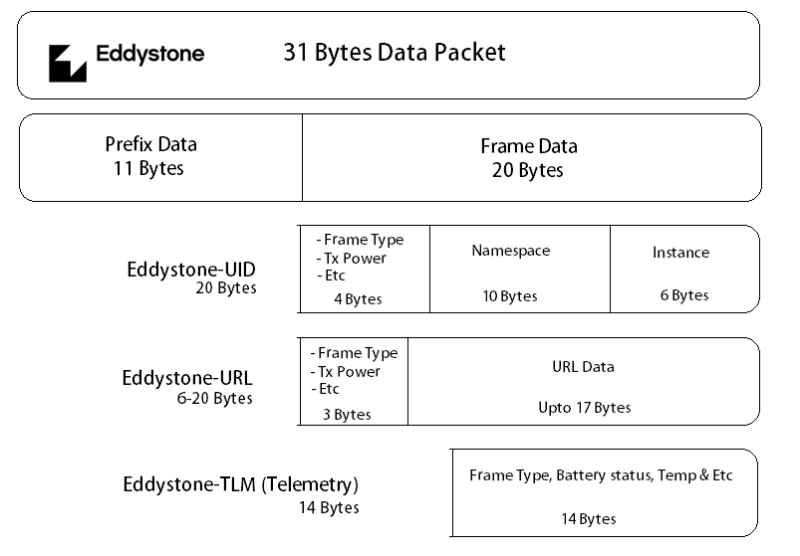
\includegraphics[width=.6\textwidth]{figures/eddystoneProtocol.png}
\caption[abs]{Tipos de paquetes Eddystone con su respectivo tamaño.\\
{\scriptsize (Fuente: \citep{protocolosBeacon})}}
\label{fig:eddystone}
\end{figure}

\begin{figure}[ht!]
\centering
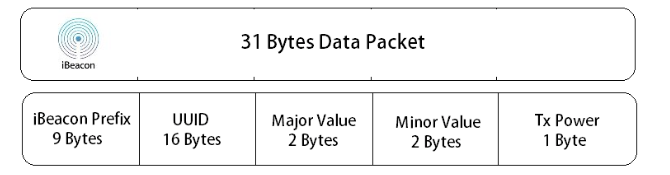
\includegraphics[width=.6\textwidth]{figures/ibeaconProtocol.png}
\caption[abs]{Paquete IBeacon realizado por Apple.\\
{\scriptsize (Fuente: \citep{protocolosBeacon})}}
\label{fig:ibeacon}
\end{figure}

\section{Estabilidad de la señal Bluetooth}

Las señales u ondas de radio son altamente afectadas por ruido o interferencia presente en el entorno, perdiendo asi intesidad en la señal o resultando en valores fluctuantes que causan estimaciones o eventos no esperados. Esto ocurre por ejemplo en las interferencias de señales Wi-Fi al descargar un archivo, o también en equipos Bluetooth al conectarse a un equipo de musica. La localizacion en interiores al depender igualmente del valor de Received Signal Strength Indicator( RSSI) o intensidad de la señal recibida; se ve ampliamente afectado, sobre todo por el hecho de que los usuarios estan caminando y en un entorno cambiante. El RSSI habitualmente se expresa en en dBm para medir la potencia obtenida por una señal recibida. Su valor mayor teorico es 0 dBm y la escala corresponde a valores negativos, en donde mas negativo implica una mayor perdida de señal.

El cuerpo humano asi como otros objetos, provoca una perdida de señal debido a la atenuacion de esta, debido a la reflexión o refracción que ocurre segun los materiales en donde la señal incide. El cuerpo humano provoca absorcion de las señales y disminución de la calidad de estas. Ademas, la propagación multicaminos es un efecto latente en todas las ondas de radio, en donde las ondas llegan al receptor por diferentes caminos y diferentes tiempos, provocando interferencia constructiva o destructiva. Este fenómeno habitualmente ocurre por los medios en donde se transportan las ondas y el entorno como tal, provocando que la señal obtenida difiera de la original manifestando ruido e interferencia, disminuyendo asi la calidad e intensidad de esta.

Para corroborar como afectan estos fenómenos a la intensidad de la señal recibida por Beacons Bluetooth, se realiza una prueba en donde se pueden visualizar los efectos de obstruccion en la señal. Para realizar esta prueba se utiliza un telefono celular con una pequeña aplicacion la cual es capaz de percibir las señales Bluetooth emitidas por un dispositivo Beacon en sus cercanías. Cada cierto tiempo se registran los valores RSSI percibidos y se escriben en un archivo de texto para posteriormente ser procesados. Se mide la señal durante 3 minutos con una linea de visión limpia, es decir, sin obstrucciones o interferencias entre ambos dispositivos. Luego, una persona camina entre la linea de visión y también permanece quieto en ella, obstruyendola completamente. La \autoref{fig:beacon_interferencia} muestran los resultados de estas pruebas.

\begin{figure}[ht!]
\centering
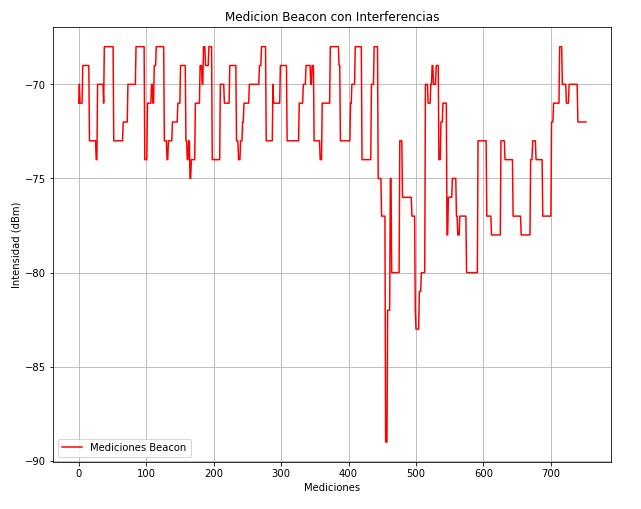
\includegraphics[width=.6\textwidth]{figures/mediciones_beacon_interferencia.jpg}
\caption[abs]{Resultados del cambio en la señal producto de una persona caminando delante de la linea entre un Beacon y un teléfono celular receptor\\
{\scriptsize (Fuente: Elaboración propia)}}
\label{fig:beacon_interferencia}
\end{figure}

Como se observa en la imagen, en un principio, la señal oscila en valores inferiores a -75 dBm, lo cual es aceptable y medianamente bueno según la escala RSSI. Posteriormente a partir de la medición 400, se introduce la aparición de la persona en la linea de propagación de la señal, con lo que inmediatamente la intensidad de la señal se reduce significativamente, incluso llegando a los limites de -90 dBm que es básicamente inestable, ya que para una conexión segura al menos se recomienda -80 dBm. Posteriormente la persona se mueve a través de la linea de visión, provocando los efectos de la gráfica, es decir, señales intermitentes y poco estables.

Todo esto demuestra principalmente que no se puede confiar completamente en el valor de la intensidad de la señal recibida, ya que es muy probable que arribe con efectos de multicamino u obstrucciones que modifican su valor durante el viaje. Este efecto es significativamente mayor en grandes distancias de viaje en las señales, lo cual sugiere que los Beacons instalados no tengan una disposicion tan distante, es decir, para obtener mejores resultados es mucho mejor una gran densidad de Beacons por superficie, lo que aumenta el costo de despliegue. Por otra parte los algoritmos de posicionamiento deben aprender a leer e interpretar este ruido, basado en patrones segun la posicion, con lo cual los algoritmos supervisados de maquinas de aprendizaje son sumamente efectivos en este ámbito.

\section{Evaluación y selección de Beacons Bluetooth}
\label{sec:seleccion}

A pesar de que en el mercado existe una gran variedad de empresas proveedoras de beacons bluetooth, hay dos que se destacan por sobre los demás y que son pioneras dentro de esta industria, estas son Estimote \citep{estimote} y Kontakt \citep{kontaktio}. Amas empresas proveen de hardware y soluciones de software ya implementadas y listas para el uso empresarias o pequeños desarrollos. Para compararlos solo se considerar los beacons estandar dentro de cada proveedor, ya que existen multiples variedades en cada segmento, sin embargo estos poseen otras cualidades como sensores de luz, temperatura, lectores NFC, UWB, o son resistentes al agua, polvo, entre otros. Para hacer un análisis justo y conciso, en este caso se obviaran estas características aunque si pueden ser utilizadas en diversos contextos. 

Para la comparativa se utilizan las características indicadas por cada fabricante y estas se resumen en la siguiente tabla:

\begin{table}[]
\centering
\caption{My caption}
\label{my-label}
\begin{tabular}{|c|c|c|}
Parametro                   & Kontakt.io                      & Estimote                             \\ \hline
Duracion de la bateria      & Hasta 4 años                    & Hasta 2 años                         \\ \hline
Rango                       & 70m                             & 70m                                  \\ \hline
Procesador                  & 32-bit ARM® Cortex™ M0 CPU core & ARM® Cortex®-M4 32-bit processor FPU \\ \hline
Sensibilidad                & -93dBm                          & -96 dBm                              \\ \hline
Velocidades                 & 250kBs, 1Mbs, y 2Mbs            & 1 Mbps (2 Mbps soportado)            \\ \hline
Memoria                     & 256KB flash 16KB RAM            & 512 kB Flash memory 64 kB RAM memory \\ \hline
Transmission power          & -30dBm to 4dBm                  & -20 to +4 dBm                        \\ \hline
Bateria                     & 2 x 1.000mAh CR2477             & 1 x CR2477 – 3.0V                    \\ \hline
Bluetooth                   & Bluetooth® 4.2 LE standard      & Bluetooth® 4.2 LE standard           \\ \hline
Espesor                     & 15mm                            & 17mm                                 \\ \hline
Peso                        & 35 gr                           & 30 gr                                \\ \hline
Paquete ibeacon y eddystone & 1 a la vez                      & 1 a la vez                           \\ \hline
Paquetes adicionales        & telemetria                      & telemetria                           \\ \hline
Sensores adicionales        & Temperatura                     & movimiento, temperatura              \\ \hline
Bateria reemplazable        & Si                              & Si                                   \\ \hline
Numero de beacons           & 3                               & 3                                    \\ \hline
Precio                      & 60 USD                          & 59 USD                               \\ \hline
\end{tabular}
\end{table}

La tabla (numero de tabla) muestra que ambos equipos son muy similares en teoría, ademas ambos presentan kits de desarrollo de software para las principales plataformas, ya sea web, aplicaciones móviles como Android e IOS como también permiten la integración de la infraestructura en la nube. Para determinar entonces la elección, es necesario realizar pruebas en ambos hardware, sin embargo estas pruebas ya han sido realizadas en múltiples ocasiones por investigadores como se aprecia en \citep{comparativaKontakt} en donde se realizaron pruebas de fluctuación en las señales para ambos equipos. La prueba consiste en poner beacons kontakt y estimote a una distancia de 2 metros de un dispositivo móvil que registra la señal. Ambas configuraciones son idénticas en los equipos y las mediciones fueron realizadas cada 500ms. Los resultados de las pruebas indican que los beacons de Kontakt tienen muchas menos fluctuaciones y la señal permanece estable por mucho mas tiempo, lo que es un indicio que pueden ser mucho mas factibles en la localización en tiempo real.


\section{Algoritmos de \textit{Machine Learning}}

Para determinar la posición del dispositivo móvil, es necesario contar con un algoritmo que pueda inferir la posición del usuario basado en las señales percibidas por los distintos Beacon. Para ello en este trabajo se utilizaran los denominados algoritmos de aprendizaje automático o \textit{machine learning}. En términos generales los algoritmos de aprendizaje automático corresponde a una rama de la inteligencia artificial en donde su objetivo principal es lograr que los computadores puedan aprender por si mismas, sin necesidad de programar su comportamiento explicitamente. Para lograr esto, se entrenan los diferentes algoritmos mediante información suministrada en forma de ejemplos según el tipo de resultado que se espera. El auge de este tipo de técnicas ocurre con la llegada del internet y los grandes volúmenes de datos, ya que para resolver ciertos problemas como clasificación de imágenes, los algoritmos convencionales son NP-Hard, es decir, su complejidad computacional es muy alta o desconocida, por lo tanto no es computacionalmente computable en un tiempo razonable, por lo que las técnicas de aprendizaje automático o heuristicas pueden entregar resultados positivos con una alta precisión sin necesidad de programar un algoritmo especifico a cada problema.

Para la utilización de estos tipos de técnicas, es necesario una representación adecuada de los datos acorde al problema que se requiere resolver, para ello se deben describir los datos, por ejemplo los pixeles de una imagen como una matriz de atributos, es decir, cada registro o fila es una imagen y cada atributo, campo o columna de la matriz es un pixel de la imagen. La representacion de los datos es de vital importancia para obtener unos resultados positivos.

Dentro del aprendizaje automático se distinguen dos tipos de técnicas de las mas conocidas, las cuales son aprendizaje supervisado y no supervisado. El aprendizaje supervisado corresponde a deducir una función o mapeo según los datos con los cuales es entrenado el modelo, para ello al momento de entrenar se debe suministrar pares de objetos, en donde una componente son los datos de entrada, por ejemplo los pixeles de una imagen; y en la segunda componente se suministra la clase de esta imagen, que puede corresponder por ejemplo al objeto presente en la imagen, como un tipo de animal o automóvil, dependiendo del problema a tratar. Entonces la función es capaz de determinar un valor numérico (regresión) o una etiqueta(clasificación) para nuevos datos no vistos anteriormente. Por lo anterior, es necesario que el modelo generalice adecuadamente y no se sobre ajuste a los datos de entrenamiento, es decir, solo sea capaz de inferir correctamente sobre el conjunto de entrenamiento y no para nuevos datos. Mientras mas datos son suministrados, mas fácilmente es para las técnicas de aprendizaje automático predecir correctamente para nuevos datos.

Estos algoritmos son tipicamente implementados en dos fases. En la primer fase, denominada fase de entrenamiento o \textbf{training phase}, los datos son recopilados y manipulados de forma tal que pueden ser suministrados a los algoritmos de aprendizaje automatico, de esta forma, los algoritmos pueden ``aprender" patrones de los datos y clarificarlos. En la segunda fase, denominada fase de pruebas o \textbf{testing phase}, nuevos datos no vistos previamente son probados en el algoritmo entrenado en la primera fase, para dilucidar la efectividad del modelo construido.

A lo largo de este trabajo se utilizan muchos tipos de algoritmos, sin embargo a continuación se procede a describir los mas relevantes y que serán mayormente utilizados en la localización en interiores, ya que a lo largo de investigaciones previas han demostrado buenos resultados en problemas similares.

\begin{figure}[ht!]
\centering
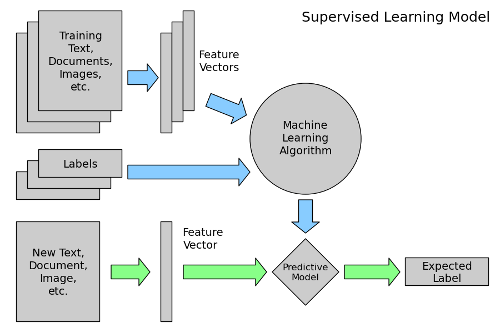
\includegraphics[width=.6\textwidth]{figures/image_machinelearning.png}
\caption[abs]{Esquema básico del funcionamiento de las técnicas de aprendizaje automático\\
{\scriptsize (Fuente: \cite{machineLearningBasic})}}
\label{fig:machineLearningBasic}
\end{figure}

\subsection{K-Nearest Neighbor}

El método K-Nearest Neighbor o método de los \textbf{k} vecinos mas cercanos, abreviado también como \textbf{\textit{k-nn}} es un metodo d eclasificacion y regresion supervisada, muy simple pero a la vez poderoso, ya que es no parametrico, es decir, no es necesario configurar parámetros del modelo, por lo que entradas de datos similares deben tener salidas de datos similares. Este método estima la funcion de densidad $F(\frac{x}{C_{j}}$ de las predictorias $x$ (datos de entrada) por cada clase $C_{j}$. En el proceso de aprendizaje no se hace ninguna suposición sobre el la distribución de las variables predictorias.

Aunque es un algoritmo supervisado, su fase de entrenamiento es muy acotada, enfocandose mayormente en la fase de pruebas, ya que todo el esfuerzo realizado por este algoritmo es hecho sobre la marcha, es decir, mientras se ejecuta estima la mejor prediccion en cada instante de la fase de entrenamiento, por lo que también se habla de un algoritmo de aprendizaje basado en instancias.

Los datos son representados por vectores en un espacio multidimensional, en donde cada ejemplo posee $p$ atributos y existen $q$ clases para clasificarlos. Luego el algoritmo esencialmente separa el espacio multidimensional en regiones, en donde un nuevo dato sera clasificado como perteneciente a una clase $C$ siempre y cuando esta clase sea la mas frecuente entre los $k$ vecinos mas cercanos al dato en cuestión. Para medir la distancia entre datos o vectores, se puede utilizar distancia euclideana, manhattan, Chevyshev, distancia del coseno, entre otras. Luego, por ejemplo para la distancia euclideana se tiene la siguiente formula:

\[ d(x_{i}, x_{j}) = \sqrt{\sum_{r=1}^{p}(x_{ri} -x_{rj})^{2}} \]

Luego, un dato esta descrito como:

$$ x_{i} = (x_{1i}, x_{2i}, ..., x_{pi}) \in X$$

Luego la fase de entrenamiento del algoritmo consiste en almacenar los valores y sus características, así como las etiquetas. En la fase de clasificacion, se mide la distancia entre el nuevo vector y los datos de entrenamiento previamente almacenados y se seleccionan los $k$ ejemplos mas cercanos, para posteriomente ser clasificado segun la clase que mas se repite dentro del conjunto de elementos seleccionados.

Este algoritmo tiene un problema al suponer que todos los atributos son igualmente relevantes, ya que al usar la distancia euclideana, todos valen lo mismo, por lo que un atributo relevante tiene el mismo ``peso'' que uno irrelevante. Sin embargo este problema no ocurre en la clasificación utilizando Beacons, ya que cada una de las señales emitidas por distintos Beacons es igual de relevante y no importa su peso.

Un problema relevante al tratar con algoritmos basados en distancia es el llamado efecto de la ``maldicion de la dimensionalidad'' o \textit{curse of dimensionality}, el cual hace referencia al problema de encontrar patrones en espacios de altas dimensiones, ya que mientras mas alta es la dimensionalidad de los datos, mas dispersos están y para seguir obteniendo resultados buenos, es necesario suministrar una cantidad de datos que crece exponencialmente. Ademas, al ser tan grande el espacio dimensional, es mucho mas complejo encontrar patrones o regiones para lograr una correcta clasificación.

Por ultimo, al tener muchos atributos, y muchos datos de entrenamiento, k-nn se torna muy lento, ya que para inferir un nuevo dato de prueba, requiere recorrer todos los datos de entrenamiento, provocando que el tiempo de procesamiento aumente significativamente a medida que aumenta el numero de datos en el \textit{dataset}. Esto es un punto relevante en el posicionamiento indoor, ya que en un simple despliegue de una infraestructura de Beacons por ejemplo en un centro comercial, se deben almacenar miles de puntos de referencia, con lo cual k-nn puede reducir su \textit{performance} y demorar demasiado, lo cual es critico en posicionamiento en tiempo real.

La \autoref{fig:knn} muestra el funcionamiento de k-nn y como el valor seleccionado de $k$ puede afectar en la clasificación.

\begin{figure}[ht!]
\centering
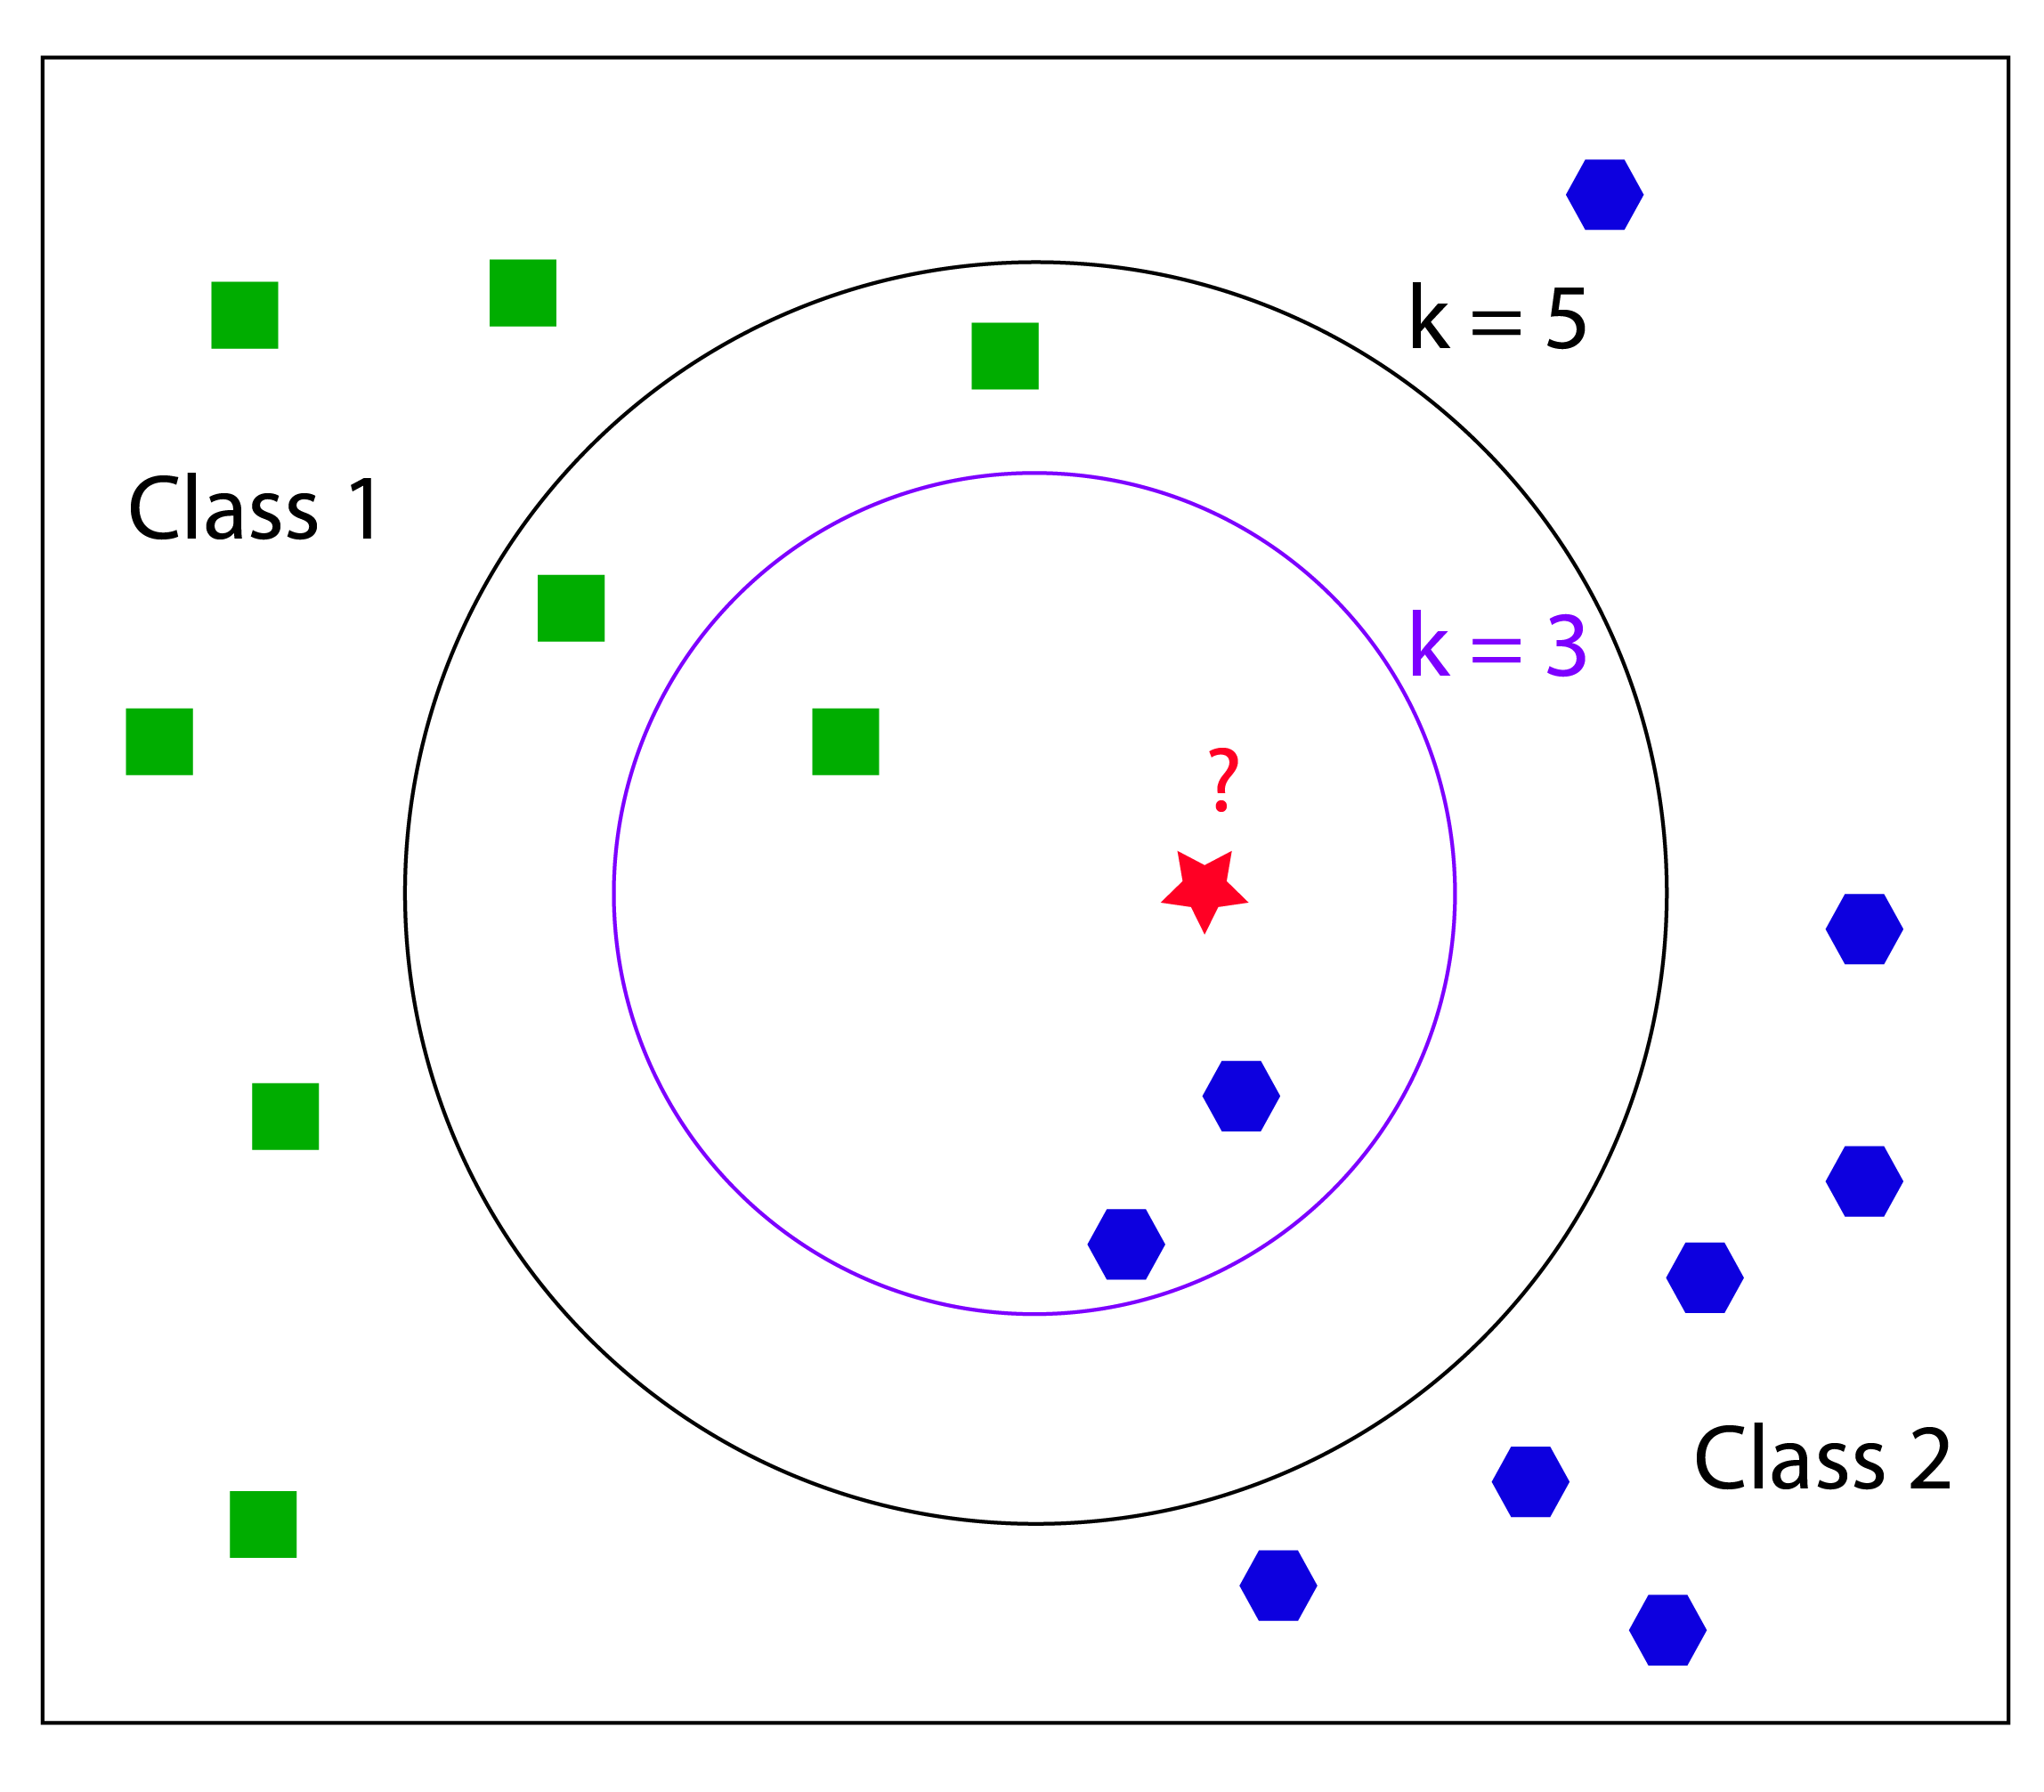
\includegraphics[width=.6\textwidth]{figures/knn.png}
\caption[abs]{Ejemplo de clasificación utilizando k-nn con $k=5$ y $k=3$}
\label{fig:knn}
\end{figure}

\section{Support Vector Machines}

Otro de los algoritmos mas utilizados en aprendizaje supervisado corresponde al denominado \textit{support vector machine}(SVM) o maquina de vectores de soporte. Ese algoritmo es sumamente utilizado sobre todo en problemas de clasificación, regresión y \textit{detección de outliers}. Una maquina de vectores de soporte construye un hiperplano o un conjunto de ellos, en un espacio de alta dimensionalidad o dimensionalidad infinita, el cual puede ser utilizado para clasificación. Intuitivamente, un buen hiperplano separador es aquel que logra maximizar la distancia a cada ejemplo de entrenamiento mas cercano a el, de cada clase, lo cual se conoce como margen funcional, entonces mientras mas grande es este margen, menor es el error de generalización del clasificador, es decir, permite mayor generalización para nuevos datos sin definir un margen estricto que solo se adapte a los datos de entrenamiento. Posteriormente para clasificar nuevos ejemplos, la SVM ubica este nuevo punto en una región del espacio que corresponde a una clase, segun su distancia y posicion respecto al hiperplano definido en la fase de entrenamiento.

\begin{figure}[ht!]
\centering
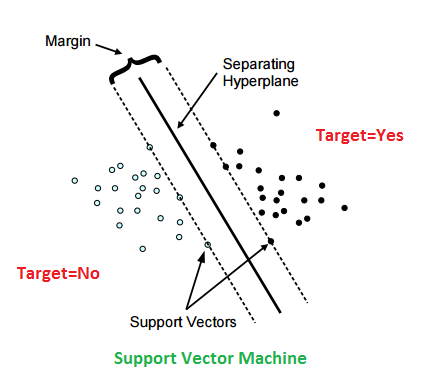
\includegraphics[width=.6\textwidth]{figures/SVM-Planes.png}
\caption[abs]{Ejemplo SVM en dos dimensiones, en donde se muestran los vectores de soporte y el hiperplano que logra la máxima separación}
\label{fig:svm}
\end{figure}

Como muestra la \autoref{fig:svm}, este hiperplano logra una separación en un espacio de dos dimensiones, lo cual es adecuado en clasificación binaria. Aunque la formulación matemática es idéntica, para resolver SVM en problemas de multiclases, es necesario escoger un esquema de resolucion. Una de las aproximaciones mas utilizadas de resolucion es reducir el problema de multiclasificacion en muchos problemas de clasificacion binaria. Para ello se utilizan formulaciones conocidas en la inteligencia artificial como \textit{one-vs-all} o es quemas de votos como \textit{one-vs-one}. La formulación matemática se muestra a continuación:

Dado un conjunto de vectores de entrenamiento $x_{i} \in I\!R ^{p}, \rm i = 1, ..., n$ en dos clases y un vector $ y  \in \{1, -1\}^{n}$ , SVM resuelve el siguiente problema de optimizacion:

$$ \underset{w, b, \zeta}{\mathrm{min}} \, \frac{1}{2} w^{T}w + C
\sum_{i=1}^{n} \zeta_{i}$$

sujeto a: 

\begin{align}
y_{i} ( w^{T} \phi(x_{i}) + b \geq  1 - \zeta_{i}, \\ 
\zeta_{i} \geq 0, \\
i = 1, ... , n
\end{align} 

En su forma dual de problema de programacion lineal, este problema es puede ser expresado como:

$$ \underset{\alpha}{\mathrm{min}} \, \frac{1}{2} \alpha^{T} Q \alpha - e^{T} \alpha$$

sujeto a: 

\begin{align}
y^{T} \alpha = 0, \\
\quad 0\leq \alpha_{i} \leq C, \, i = 1, ..., n 
\end{align} 

En donde $e$ es el vector de unos, $ C > 0$ es el limite superior, y $ Q$ es una matriz semidefinida positiva de tamaño $ n$ por $ n$, $ Q_{ij} = y_{i} y_{j} K(x_{i}, x_{j})$ en donde $K(x_{i}, x_{j}) = \phi(x_{i})^{T} \phi(x_{j})$ se denomina el kernel y es sumamente importante en SVM, ya que este permite llevar desde un espacio en donde la separación de las clases no es tan clara, a un espacio de dimensiones muy grandes o infinitas, en donde la separación se vuelve mucho mas obvia.

Finalmente, la función de decisión corresponde a:

$$ sgn(\sum_{i=1}^{n}y_{i} \alpha_{i}K(x_{i}, x) + \rho)$$ 

La relevancia del kernel es lo que torna a SVM muy factible en problemas de clasificación, ya que permite llevar los datos de un espacio finito, en donde no son linealmente separables, a un espacio de dimension infinita en donde si pueden ser separados linealmente, lo cual es conocido como \textit{kernel-trick}. Ademas, como solo se utilizan funciones kernel que utilicen producto punto, la operación de llevar estos datos al nuevo espacio es eficiente y de bajo costo computacional. Para realizar el kernel trick, cada producto punto es reemplazado por una funcion kernel de carácter no lineal. El kernel mas utilizado es RBF o radial basis function el cual es definido como:

$$ K(x_{i}, x_{j}) = exp(- \gamma \left\|{ x_{i} - x_{j}}\right\|^2) , \, \gamma > 0$$

Luego, utilizando este kernel, se debe escoger el parametro $\gamma$ y el parametro $ C$ adecuado, los cuales son muy importantes en una correcta generalización del SVM. Habitualmente SVM al ser un hiperplano de máxima distancia a cada clase, es muy estricto en la clasificación, lo cual no siempre es lo ideal, debido a que pueden existir \textit{outliers} debido a ruido, afectando a toda la clasificación. El hiperparametro $C$ ayuda en este sentido, con lo que se denomina \textit{soft-margin}, es decir, un margen mas permisivo, que clasifica de manera errónea algunos ejemplos de entrenamiento, buscando la generalización del SVM.

Por otra parte, el hiperparametro $\gamma$ define que tan lejos alcanza la influencia de un ejemplo de entrenamiento por si solo, es decir, puede ser visto como el inverso del radio de influencia de los ejemplos de entrenamiento escogidos como vectores de soporte. Un valor pequeño de $\gamma$ producirá un largo alcance, definiendo zonas de clasificación muy amplias, con lo cual no se aprecia completamente la forma o patrón de estas. Por otra parte un valor grande, provoca demasiada separación, aislando cada ejemplo de entrenamiento.

\section{Redes Neuronales y Deep learning}

Uno de los campos de investigación con mayor auge en el ultimo periodo, es todo lo relativo a los avances en redes neuronales, particularmente \textit{deep learning}.  La base de estos modelos computacionales son, como indica su nombre, las neuronas y su funcionamiento en el cerebro y el sistema nervioso. El cerebro, en particular el sistema visual o corteza visual primaria, es el responsable de reconocer patrones, y lo hace de manera tal en que una imagen es dividida y analizada a traves de muchas capas, disminuyendo la complejidad en cada una de ellas para ir de lo macro a lo micro, pudiendo asi establecer patrones de menor escala y localidades en la imagen que ayuda a distinguir de que se trata el objeto visualizado.

Cada unidad neuronal esta conectada a las neuronas de la capa siguiente y ellas pueden aumentar o inhibir el estado de las neuronas en la capa siguiente. Estos sistemas por lo mismo, pueden aprender solos, solo se debe suministrar un numero adecuado de ejemplos para el entrenamiento.

Cada activacion de la neurona en la capa siguiente depende de los pesos $w$ y el sesgo o \textit{bias} $b$. Los pesos multiplican a las entradas en cada conexion, y el bias es el limite, de donde se establece si la suma ponderada de las entradas con los pesos es mayor o menor que el bias, entonces la neurona se activa.

\begin{figure}[ht!]
\centering
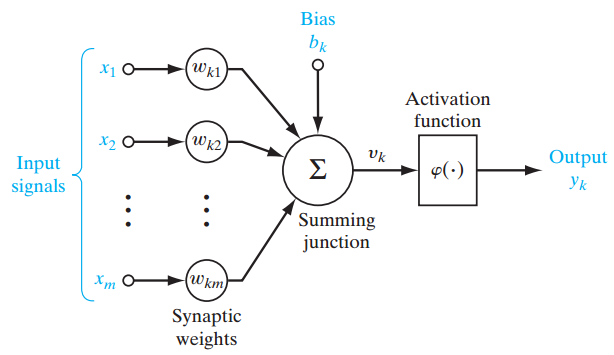
\includegraphics[width=.6\textwidth]{figures/SLP.png}
\caption[abs]{Esquema basico de single layer perceptron\\
{\scriptsize (Fuente: \cite{slp})}}
\label{fig:slp}
\end{figure}

La \autoref{fig:slp} muestra como cada entrada es multiplicada por su respectivo peso, y la suma ponderada se suma con el bias, para luego utilizar la funcion de activacion y obtener la salida , la cual describe que tanto aporta esta neurona, la cual sera el nuevo input para la siguiente capa. La neurona perceptron queda descrita como:

\begin{equation}
output = \left\{ \begin{array}{lcc}
             0 &   si  & w \cdot x + b \leq 0 \\
             \\ 1 &  si & w \cdot x + b > 0 \\
             \end{array} \right.
\end{equation}

En donde $ w\cdot x = \sum_{j} w_{j} x_{j} $ con $w$ y $x$ son vectores en donde sus componentes son los pesos y las entradas respectivamente, y el numero de neuronas en la capa corresponde a $j$. A pesar que este modelo sirve para problemas simples, no funciona de buena manera en problemas altamente no lineales. 

La neurona mas utilizada es la denominada neurona sigmoid. Estas neuronas son similares a las neuronas perceptron(primeras neuronas inventadas), pero pequeños cambios en sus pesos y sesgos, provocan pequeños cambios en las salidas, lo cual las hace mucho mas útiles y diversifican muy bien la información a través de la red. La funcion de activacion de este tipo de neuronas corresponde a la funcion sigmoid, y ayuda a resolver problemas estrictamente no lineales. Luego el output $y_{k}$ viene dado por:


$$ \sigma( w \cdot x + b) = \frac{1}{1 + exp(- \sum_{j} w_{j}x_{j} - b)}$$

Luego el procedimiento por el cual aprende la red corresponde a un algoritmo denominado \textit{backpropagation} el cual puede computar los pesos y bias adecuados para la red, con el objetivo de entrenarla y definir los mejores hiperparametros para posteriomente clasificar de manera correcta nuevos ejemplos. El algoitmo de backpropagation consiste en los siguientes pasos:

\begin{enumerate}
\item \textbf{Input:} Iniciar la correspondiente activación de la capa de entrada

\item \textbf{Feedforward:} Computar las salidas de cada neurona de las capas ocultas. Finalmente computar la salida de la capa de salida.

\item \textbf{Output error:} Computar los errores de la capa final o capa de salida

\item \textbf{Backpropagation:} Propagar el error de la capa de salida a la capa anterior oculta. Repetir para todas las capas hasta llegar a la capa de entrada.

\item \textbf{Output:} Calcular el gradiente de la función de costo, para luego actualizar los pesos y bias.

\end{enumerate}

Para calcular el gradiente se utiliza gradiente descendente, y entonces, cada iteracion consiste en atravesar la red hacia adelante, computar el error y volver para propagar el error y computar los ajustes y actualizaciones a los hiperparametros. Este algoritmo ha logrado un gran avance en las redes neuronales artificiales permitiendo entrenarlas de manera mucho mas rápida, logrando grandes resultados.

Las redes neuronales obtienen buenos resultados en gran parte de los problemas, pero para problemas demasiado complejos el concepto de multilayer perceptron, es decir, el modelo estandar de redes neuronales, no es suficiente. Para ello, ha surgido el concepto de \textit{deep learning} o aprendizaje profundo. Estas redes son similares a las redes normales, pero poseen mas de una capa escondida y ademas se han desarrollado otros algoritmos para resolverlas eficientemente. 

\begin{figure}[ht!]
\centering
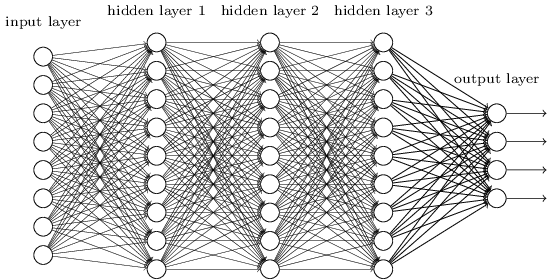
\includegraphics[width=.6\textwidth]{figures/deep.png}
\caption[abs]{Red neuronal profunda con multiples capaz escondidas\\
{\scriptsize (Fuente: \cite{slp})}}
\label{fig:slp}
\end{figure}

Para resolver este tipo de redes profundas existen muchos acercamientos, y cada día nacen nuevas formas de resolución. Las formulaciones matemáticas son muy extensas, pero en términos generales los algoritmos de backpropagation y gradiente descendente son las bases fundamentales de resolución, a pesar que necesitan modificaciones para que la red no se quede atascada en ciertas capas, cosa que habitualmente ocurre en redes profundas.

\section{Descripción del \textit{framework} de posicionamiento}

Para la elaboración del sistema de posicionamiento, se utiliza la técnica de fingerprint discutida en el estado del arte, la cual mediante la utilización de un mapa de señales, también denominado \textit{radiomap}, puede inferir la posición de un usuario utilizando algún algoritmo de localización. Como el objetivo de este trabajo es determinar los mejores algoritmos de maquinas de aprendizaje para posicionamiento indoor utilizando bluetooth low energy, es necesario establecer un marco de trabajo mediante el cual se pueda llevar a cabo esta tarea.

Lo primero a tener en consideración, es que se deben utilizar dispositivos Bluetooth Low Energy, lo cuales realizan la función de access point(AP) y que serán los responsables de emitir la señal RSSI. Luego, el procedimiento se divide en las dos clásicas etapas de fingerprint, es decir, fase \textit{offline} y fase \textit{online}

\subsection{Fase Offline}

Para la generación del radiomap, se debe crear un tipo de aplicación que sea capaz de recolectar los vectores RSSI en diversos puntos dentro del lugar de experimentación. Esta aplicación debe ser simple y permitir la adición de nuevos puntos fingerprint. Por lo tanto, esta es una tarea muy importante, ya que estos datos se implementaran los algoritmos de maquinas de aprendizaje. El periodo y frecuencia de los datos se debe determinar experimentalmente. Para ello, cada punto a colectar, representa un punto en el espacio $2-dimensional$, es decir, un punto dentro del plano. Para generar la grilla, es necesario tener la posicion exacta, que corresponde a la etiqueta de cada punto mapeado. Entonces, se formara una grilla de múltiples puntos con sus respectivos fingerprints leídos. Cabe destacar que los puntos de referencia en donde se toman los datos, no necesariamente deben estar equiespaciados, pero de esta manera es mucho mas simple formar la grilla, ya que cada punto de medición puede corresponder al centro de un cuadrado de determinadas dimensiones. La \autoref{fig:fingerprints} muestra la grilla a desarrollar, con un punto de referencia y su respectivo vector RSSI expresado en dBm.

\begin{figure}[ht!]
\centering
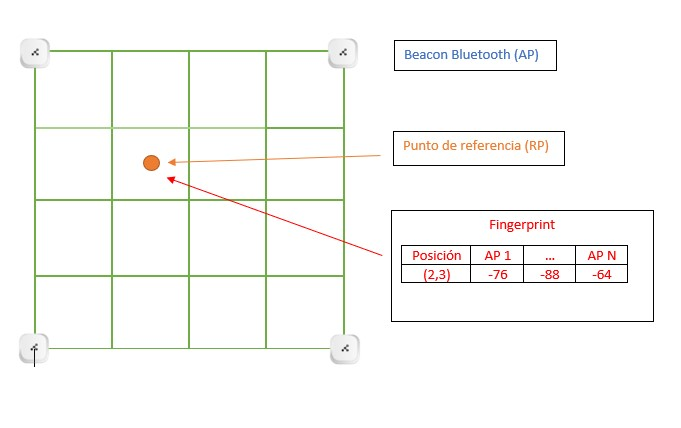
\includegraphics[width=.6\textwidth]{figures/fingerprints.jpg}
\caption[abs]{Ejemplo de grilla utilizada, con sus puntos de referencia y los fingerprints leidos, que corresponden a vectores de señales RSSI\\
{\scriptsize (Fuente: Elaboración propia)}}
\label{fig:fingerprints}
\end{figure}

Con los datos registrados, se debe crear la base de datos que almacenara estos fingerprints, ya que desde ahí es posible analizar los datos y mantener su persistencia. Posteriormente, con estos datos se crea el radiomap respectivo, es decir, asociar un vector de señales RSSI, en donde cada componente representa la intensidad recibida proveniente de un access point, a cada posicion en donde se colectaron los datos. El numero de fingerprints depende del numero de posiciones en donde se colectan los datos, y también de cuantos ejemplos se obtienen en cada una de estas posiciones. La tabla ejemplifica la estructura del radiomap a contruir:

\begin{table}[]
\centering
\caption{My caption}
\label{my-label}
\begin{tabular}{|c|c|c|c|c|}
\hline
Posicion & AP 1 & AP 2 & ... & AP N \\ \hline
(3,3)    & -65  & -70  & ... & -95  \\ \hline
(6,6)    & -80  & -50  & ... & -76  \\ \hline
\end{tabular}
\end{table}

Cabe destacar que los algoritmos de maquinas de aprendizaje a pesar que pueden resolver para problemas multivariados, es decir, predecir para dos variables, en este caso $(x,y)$ como un punto; es mucho mas sencillo separar esto en dos problemas, vale decir, un algoritmo de maquina de aprendizaje para $x$ y otro para $y$. Otra alternativa seria asociar una clase a cada punto, es decir, numerar estos puntos de la grilla, pero el problema con esto es que se torna mucho mas complejo de aprender, debido a que se necesitarían demasiados datos para verdaderamente lograr un aprendizaje de cada una de estas clases, provocando un aumento significativo en la complejidad del problema.

Teniendo en consideración los puntos anteriormente mencionados, el siguiente paso es entrenar los algoritmos de aprendizaje a ser comparados y utilizados en el posicionamiento. Antes de el entrenamiento, es necesario de destacar que se utilizara un algoritmo de reducción de dimensional. Esto no ha sido mayormente explorado en la literatura, sin embargo puede ser de mucha utilidad a la hora del entrenamiento y la fase \textit{online}. La principal razón de utilizar estas técnicas, es que los puntos de referencia poseen una alta correlación, debido a que la onda decae según el cuadrado de la distancia, por lo que se presenta una correlación entre dos puntos adyacentes. Por otra parte, los métodos de extracción de características, pueden ayudar a agilizar la fase de entrenamiento, ya que este proceso es lento. Ademas, al ser menos componentes, en la fase online, las técnicas tardaran mucho menos tiempo en determinar la posición en tiempo real, lo cual es sumamente efectivo en técnicas como KNN.

Existen dos métodos muy conocidos mediante los cuales se puede reducir la dimensionalidad, estos son \textit{Linear discriminant analysis}(\textbf{LDA}) y \textit{principal component analysis}(\textbf{PCA}). Por un lado LDA es una tecnica habitualmente utilizado en los campos de estadisticas, reconocimiento de patrones y maquinas de aprendizaje. El objetivo de LDA es encontrar una combinación lineal de los \textit{features} o caracteristicas del dataset, las cuales separan dos o mas clases. La combinacion lineal resultante es habitualmente utilizada como clasificador o mas popularmente para reducir la dimensionalidad del dataset. LDA es similar a PCA, ya que ambos buscan combinaciones lineales que explican de mejor manera los datos, sin embargo la manera en que los realizan es diferente, ya que LDA explicitamente intenta modelar la diferencia entre las clases de datos, por lo que necesita de las etiquetas de cada clase, lo cual lo torna un metodo supervisado. Por otro lado, PCA no toma en cuenta la diferencia entre las clases, por lo que es un metodo no supervisado. Ademas LDA funciona bien en el caso de que las variables o atributos del dataset son independientes, y predicen la variable categorica o etiqueta de cada clase.

Como se menciono anteriormente, LDA maximiza la separación entre clases, es decir, la varianza entre clases o interclases. PCA por su parte, busca las componentes de la combinación lineal, las cuales maximizan la varianza en los datos, esto quiere decir, la varianza de las variables o varianza intraclases. LDA hace presunciones sobre los datos que lo vuelven mas complejo de implementar, por ejemplo, las clases deben estar normalmente distribuidas, y la covarianza de las clases debe ser igual. Por todo lo anterior, y como es necesario reducir la correlación entre los puntos adyacentes, se decide utilizar PCA como tecnica para reducir el espacio de dimensionalidad y para encontrar un espacio no correlacionado de variables. Esto es necesario, debido a que al estar tan correlacionado los puntos de referencia en la grilla, puede existir información o \textit{features} escondidos, lo cual no aumentara la \textit{accuracy} de las técnicas de machine learning, pero si mejora los tiempos de entrenamiento y en la fase online, lo cual es muy relevante en un sistema de posicionamiento en tiempo real. La correlación se debe a que como es sabido, las ondas se propagan de la siguiente forma:

$$ I \propto \frac{1}{r^{2}}$$

En donde $I$ representa la intensidad y $r$ es la distancia de propagación desde el punto de emision. Esta formula define como decae la intensidad de la señal a medida que esta se transmite en el medio según el inverso del cuadrado de la distancia. Con lo anterior, y considerando que los Beacons actuan como antenas omnidireccionales, si el RSSI de dos Beacons se mide en un punto, luego se translada a otro punto adyacente, y se mide nuevamente,  al ser la intensidad proporcional a la distancia, ambos Beacons y sus lecturas mantienen una correlación lineal, ya sea positiva o negativa, ya que ambos aumentan o disminuyen en un mismo valor según la distancia obtenida, siempre y cuando esta sea pequeña o ambas señales se propaguen en la misma dirección espacial en un vecindario determinado. Esto se conoce tradicionalmente como correlación espacial de las señales.

Como la técnica elegida es PCA, a continuación se procede a describir como funcionara específicamente para el problema de fingerprint. PCA, busca la proyección sobre la cual los datos queden mejor representados en términos de mínimos cuadrados. Esta convierte un conjunto de variables posiblemente correlacionadas en un conjunto de variables sin correlación lineal, las cuales se denominan componentes principales. PCA construye una transformacion lineal que escoge un nuevo sistema de coordenadas para el conjunto original de los datos, escogiendo la varianza mayor de los datos como primera componente en el nuevo sistema de referencia, la segunda varianza mas grande como segunda componente y asi suscesivamente. Para ello se requiere la matriz de covarianzas, mediante la cual es posible encontrar los vectores propios de la misma, que funcionan como base para las nuevas coordenadas a traves de la transformacion lineal y asi reducir la dimensionalidad.

PCA resuelve el problema de la alta dimensionalidad del radiomap construido, combinando los \textit{features} mediante una transformacion lineal en un espacio no correlacionado, es decir, un espacio ortogonal de vectores( vectores propios), utilizando la matriz de covarianza de los datos de entrenamiento de tamaño $ M \, x \, M$ . Luego, este radiomap de señales RSSI es proyectado en el espacio no correlacionado en la dirección de la varianza mas alta. La seleccion respectiva de componentes principales se basa en las varianzas mas grandes, es decir, segun los valores propios mas grandes (proyeccion de la transformación). Por lo anterior, los valores propios representan la información de las componentes principales.

El espacio característico es generado mediante un conjunto de $M$ lecturas RSSI por posición o punto de referencia, lo cual corresponde a un vector $x_{i}$ de tamaño $ 1 \, x \, M$ como vector fila, donde $ M$ es menor a $ N$, y con $ N$ el numero de ejemplos de entrenamiento.

Luego, el espacio característico posee una media:

$$ \overline{x} = \sum_{i=1}^{N} \frac{x_{i}}{N} $$

Por ende, la matriz de covarianzas puede ser descrita como:

$$ C_{r} = \sum_{i=1}^{N} (x_{i} - \overline{x})^{T}(x_{i} - \overline{x}) = X^{T}X$$

Cabe destacar que la matriz de covarianzas es simetrica y de tamaño $M \, x \, M$, por lo cual posee $M$ valores propios.

Sean los valores propios $ \{ \lambda_{1}, \lambda_{2}, ..., \lambda_{M} \} $ ordenados en orden descendiente, con sus correspondientes vectores propios normalizados $ \{ V_{1}, ... , V_{M} \} $ . Según la formula de valores y vectores propios para matrices debe cumplirse entonces:

$$ C_{r} V_{i} =  \lambda_{i} V_{i}$$
$$ \lambda_{1} \geq \lambda_{2} \geq ... \geq \lambda_{M}$$

Como se menciona anteriormente, los vectores propios $ \{ V_{1}, ... , V_{M} \} $ son no correlacionados y ortonormales, por lo que forman un espacio característico.

Con todo lo anterior, es posible proyectar el radiomap en el nuevo espacio característico. Obviamente, si se proyecta sobre todas las componentes no existe un cambio, ya que se presenta la misma información, por lo cual es necesario determinar los valores propios mas relevantes y que aportan mayor información(varianza) a los que no. Para la selección entonces de las componentes principales se toma en cuenta entonces la información contextual y el error que cada componente ha aportado. No existe manera automática de determinar el numero adecuado de componentes principales, sin embargo en la experimentación es discutida una forma de poder llevar a cabo esta tarea. 

Luego, el nuevo radiomap no correlacionado $Z$ es calculado proyectando $X$ en el espacio característico reducido $W$, el cual representa una combinación lineal de los vectores propios seleccionados, asociados a los valores propios mas relevantes. Finalmente, la matriz $Z$ del nuevo radiomap, con menor numero de componentes esta dada por:

$$ W = V \, \cdot \, X$$

$$ Z = X  \, \cdot \, W $$

Luego, los clasificadores de maquinas de aprendizaje son entrenados mediante la utilización del radiomap $Z$, el cual tiene componentes reducidas y no dependientes, con lo cual el entrenamiento es mucho mas rápido y se elimina la mayor parte de la información redundante al extraer la información mas relevante.

Las principales ventajas de utilizar PCA entonces, corresponde a \citep{7743586}:

\begin{enumerate}
\item PCA extrae la información importante del radiomap definido.

\item PCA reduce la matriz de datos multivariados sin perder mucha información, en donde los datos están descritos por muchas variables correlacionadas dependientes.

\item PCA reduce la complejidad mediante la disminución del numero de componentes, logrando mejorar tiempos de entrenamiento y calculo online.
\end{enumerate}


El siguiente paso entonces corresponde a entrenar los modelos definidos, que se explican en la parte experimental, los cuales son técnicas de maquinas de aprendizaje muy conocidos y que han presentado buenos resultados a lo largo de muchos problemas. Posteriormente, se seleccionan los mejores algoritmos, es decir, que presenten el mejor desempeño y son implementados. Una parte importante a definir en la etapa offline, es la manera en que los modelos de machine learning funcionaran en el dispositivo, ya que hay dos versiones posibles de implementacion, estas son utilizando un servidor o sin utilizar servidor. 

Ambas estrategias deben entrenar los algoritmos en una maquina dedicada, por el consumo de recursos que son necesarios, sin embargo una vez que los modelos estan entrenados, deben ser utilizados en el dispositivo movil. Para ello se puede exponer un servicio REST o API en donde el dispositivo movil envia una nueva lectura RSSI al servidor, posterior a esto el servidor computa y determina la posición y retorna este valor al dispositivo móvil. Esta alternativa es ideal en entornos donde siempre existe conexion a internet y redes de telefonía e internet movil. Esta alternativa es idonea, ya que es el servidor quien procesa los resultados, haciendo el posicionamiento mas expedito, ademas de utilizar menos recursos en el telefono y por lo mismo menos batería, ya que solo realiza conexiones de red de poco peso(solo transmite un vector de enteros).

En el caso de este trabajo, como se pretende utilizar en lugares donde no existe internet como mineras o estacionamientos subterráneos, la alternativa es desarrollar el entrenamiento en el servidor, pero luego portar los modelos a un dispositivo móvil. Esto es posible, debido a que la mayoria de los modelos desarrollados presentan ciertos componentes que pueden ser posteriormente replicados en otras maquinas sin necesidad de entrenar o re entrenar el modelo. 

Todos los pasos anteriores describen a grandes rasgos el proceso completo de la etapa offline, desde la recolección de datos hasta el entrenamiento e implementacion de los modelos en los dispositivos móviles.

\subsection{Fase Online}

Para la fase online se reconocen dos etapas principales, la primera es colectar un vector de señales RSSI en la posición actual del usuario, es decir, el vector de intensidad de la señal en donde cada componente representa la intensidad recibida por un Beacon o Access Point Bluetooth. La segunda etapa es proveer este vector de entrada a los algoritmos de aprendizaje supervisado. Para realizar esta tarea se deben tener en cuenta las normalizaciones realizadas y aplicar correctamente la transformación PCA del espacio característico antes de suministrar los datos a los algoritmos, ya que de otra manera las dimensiones serán incompatibles.

Para realizar esto, se debe proyectar el vector RSSI en el espacio característico de la ecuación xx, es decir $W$. Los valores proyectados en esta etapa son comparados con los modelos entrenados buscando de esta manera el valor estimado mas cercano según el nuevo radiomap. Una vez que los algoritmos de clasificación proveen el resultado de la posición física, entonces la misma aplicación de la fase offline, es utilizada para mostrar en un mapa de tiempo real la localización actual de usuario.

La fase Online es muy simple, ya que solo se deben evaluar los nuevos valores en los algoritmos, por lo que es claro que la parte mas importante de todo el proceso de fingerprint es la recoleccion adecuada de datos y el correcto entrenamiento de los algoritmos de \textit{machine learning}. Esto es de suma importancia, ya que malos datos o malos parámetros de entrenamiento, eventualmente provocan problemas hacia adelante, es decir, reducir la precisión en la fase Online afectando severamente los resultados.

A continuación, la \autoref{fig:propuesta} describe el procedimiento completo a desarrollar en este trabajo.


\begin{figure}[ht!]
\centering
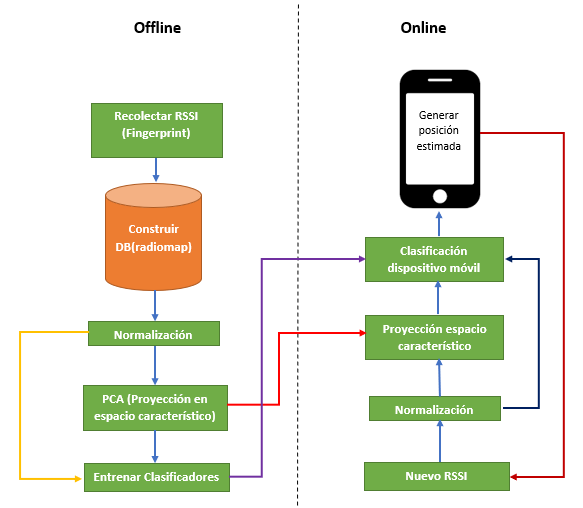
\includegraphics[width=.6\textwidth]{figures/propuesta_memoria.png}
\caption[abs]{Framework desarrollado para resolver el problema de posicionamiento en interiores\\
{\scriptsize (Fuente: Elaboración propia)}}
\label{fig:propuesta}
\end{figure}

Como se observa en la \autoref{fig:propuesta}, los datos son normalizados previamente antes de ser utilizados. Ademas la razon de la conexion entre la normalizacion y el entrenamiento de los clasificadores se debe a que se utilizaran los algoritmos de machine learning utilizando PCA y no utilizándolo, a modo de comparación en términos de tiempo y accuracy. Ademas, se ha omitido el item en donde los clasificadores ya entrenados son portados al dispositivo movil. Finalmente, hay que notar que en la fase online, el dispositivo movil genera un nuevo vector de señales RSSI, luego se transforman los datos y finalmente se clasifican, lo que genera una posicion estimada que se refleja en el dispositivo móvil. Este ciclo es constante, ya que la posición se actualiza continuamente según los parámetros definidos y frecuencia de actualización.
\chapter{Experimentación}

\section{Beacons y configuración}

Los beacons utilizados corresponden a beacons de la marca Kontakt, y el numero es 8, sin embargo, no son todos iguales. Esto ayuda a comprobar que tan efectivo es utilizar distintos modelos, ya que en entornos reales, por ejemplo en una mina, es sumamente importante contar con beacons bluetooth que se adapten al espacio físico en donde son dispuestos, por ejemplo si es necesario instalarlos en una oficina, los beacons convencionales funcionan de buena manera, sin embargo en ambientes hostiles como lugares con polvo o de difícil acceso, es necesario contar con beacons preparados para estas dificultades, los cuales tengan baterías de larga duración, sean anti polvo y agua, entre otras características. A continuación se muestra el resumen de los beacons utilizados:

\begin{enumerate}
\item \textbf{Beacon: } Beacon mas popular y de menores prestaciones. Es el clásico Beacon vendido por la compañía Kontakt. Posee una batería con duración de hasta 48 meses y un rango de 70m. Se utilizan 4 unidades.

\item \textbf{Beacon Pro: } Beacon con mas funciones de seguridad, ahorro de bateria, sensores de luz y a prueba de agua. Hasta 60 meses de bateria y rango de 70m. Se utilizan 2 unidades.

\item \textbf{Tough Beacon: } Hasta 24 meses de batería y rango de 70m. A prueba de polvo y agua. Especialmente diseñado para condiciones extremas.


\end{enumerate}

Cabe destacar que las caracteristicas basicas del \textit{Hardware} de cada beacon son las presentes en la comparativa realizada en la sección \ref{sec:seleccion}.

Foto beacons.

Lo siguiente es definir la configuración de cada Beacon. Los parámetros mas relevantes en este caso serian el \textit{TX Power} y el \textit{Beacon Interval}. En un despliegue real, lo mas relevante es disminuir los costos, que en este caso están asociado a las baterias o mas bien al cambio de estas a lo largo del tiempo. Estos dos parametros son importantes para la localización indoor, ya que el TX Power define la potencia de salida de cada Beacon y el intervalo corresponde a cada cuanto un beacon envía un mensaje a los dispositivos bluetooth cercanos. 

El valor de Tx Power afecta principalmente a tres factores claves, estos son el rango de la señal, es decir, la distancia maxima alcanzada; el segundo corresponde a la estabilidad de la señal y finalmente la bateria, aunque este ultimo factor es mayormente influenciado por el intervalo.

En terminos simples, TX Power representa que tan poderosa es la señal transmitida por los beacons en dBm y corresponde a un numero dentro del rango 0-7, donde 0 es menos poderoso y 7 el mas poderoso.Es claro que mientras mas poderoso es la señal, mayor rango alcanza y mas estable es la señal, sin embargo el consumo de energia aumenta significativamente. Para determinar el parametro TX power entonces es necesario tener en cuenta estos factores. Para el caso del posicionamiento indoor, es claro que el rango debe ser maximo, ya que de esta forma la señal de cada Beacon puede alcanzar a la gran parte de los usuarios de la zona. El otro punto significativo es establecer que tan seguido es necesario cambiar las baterias. Este punto es relevante para despliegues a gran escala y depende en gran medida de las organizaciones interesadas en desplegar un sistema de este tipo. Finalmente, es importante considerar la interferencia subyacente debido al entorno, por ejemplo objetos contundentes o multiples personas, en este caso se requiere una señal mas potente para cortar de esta forma la interferencia y pasar a traves de esta. Por los motivos declarados anteriormente se decide utilizar un TX Power igual a 7, o equivalentemente 4 dBm.

Con respecto al intervalo utilizado, es un parámetro de mucho mayor relevancia que el TX Power para el tipo de problema a resolver. Esto se debe principalmente a que el intervalo corresponde a que tan frecuente es transmitido un paquete desde un Beacon a un dispositivo móvil. Considerando que el posicionamiento debe ser lo mas cercano a  tiempo real, la información debe ser suministrada lo mas rápidamente posible. El intervalo es medido en milisegundos, y como es esperable, mientras mas pequeño el intervalo, mas recurrente es la comunicación pero mayor es el consumo de batería. A pesar de que el intervalo sea muy pequeño, muchas veces los sistemas operativos no son capaces de recibir tan rápidamente estas señales, debido a limitaciones de seguridad u otras configuraciones del fabricante como es el caso de Apple. En Android estas limitaciones no existen y por lo tanto puede recibir todas las señales, pero esto afecta de forma significativa la batería del teléfono. Por otra parte, mientras menor es el intervalo, mayor es la estabilidad de la señal, ademas el intervalo afecta significativamente a el posicionamiento en interiores, debido a que mientras mas rápido se mueve un usuario, si el intervalo es demasiado alto, su posición sufrirá saltos o cortes que no muestran realmente la ruta de desplazamiento. Si el intervalo es pequeño, puede detectar mas fácilmente la posición del usuario en cada momento con precisión de unos pocos centímetros. La  ejemplifica esta situación:


\begin{figure}[ht!]
\centering
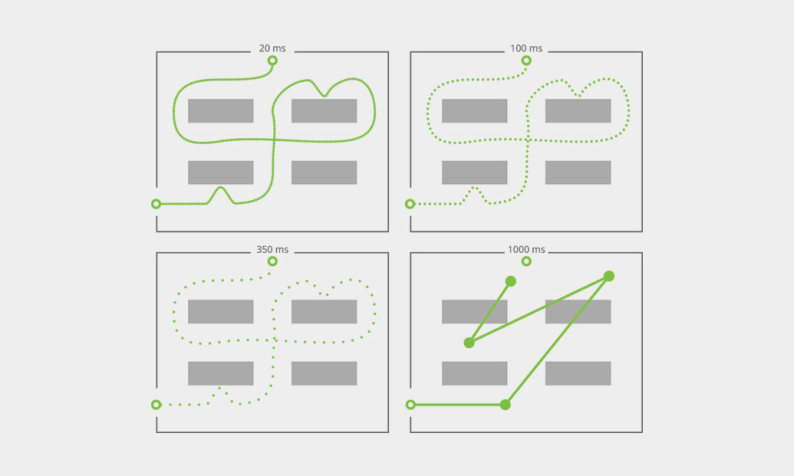
\includegraphics[width=.6\textwidth]{figures/interval.jpg}
\caption[abs]{Posicionamiento indoor con diferentes intervalos de aviso en mili segundos\\
{\scriptsize (Fuente: \cite{interval})}}
\label{fig:intervalo}
\end{figure}

Por lo anterior, es claro que los parámetros seleccionados deben ser el mayor valor posible para el TX Power correspondiente a 7, y un valor del intervalo igual a 100ms. Para configurar estos parámetros, Kontakt dispone de una aplicación para dispositivos Android. La \autoref{fig:kontaktapp1} y \ref{fig:kontaktapp2} muestran como han sido configurados los Beacons. Esta configuración es idéntica para todos los beacons utilizados.


\begin{figure}[ht!]
\centering
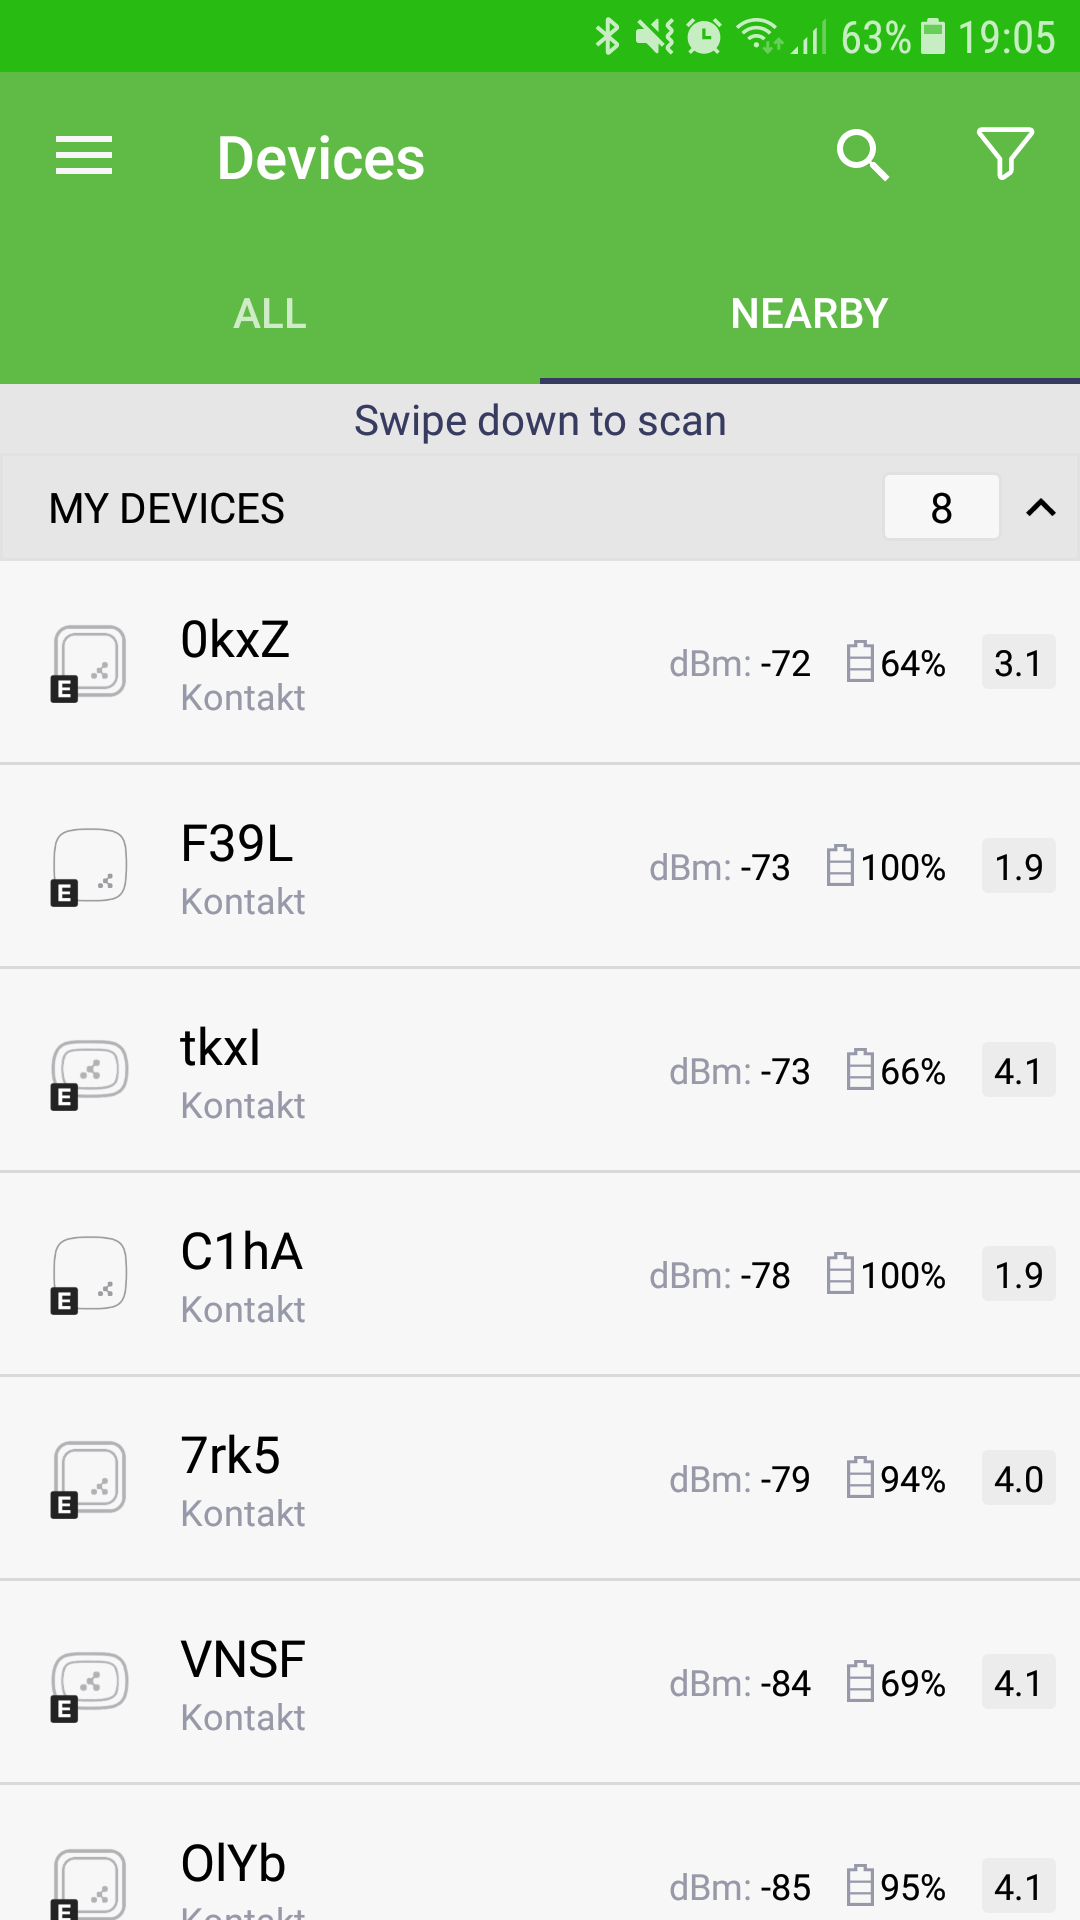
\includegraphics[width=.3\textwidth]{figures/kontaktapp1.png}
\caption[abs]{Listado de los beacons encontrados para su posterior configuración\\
{\scriptsize (Fuente: Elaboración Propia)}}
\label{fig:kontaktapp1}
\end{figure}

\begin{figure}[ht!]
\centering
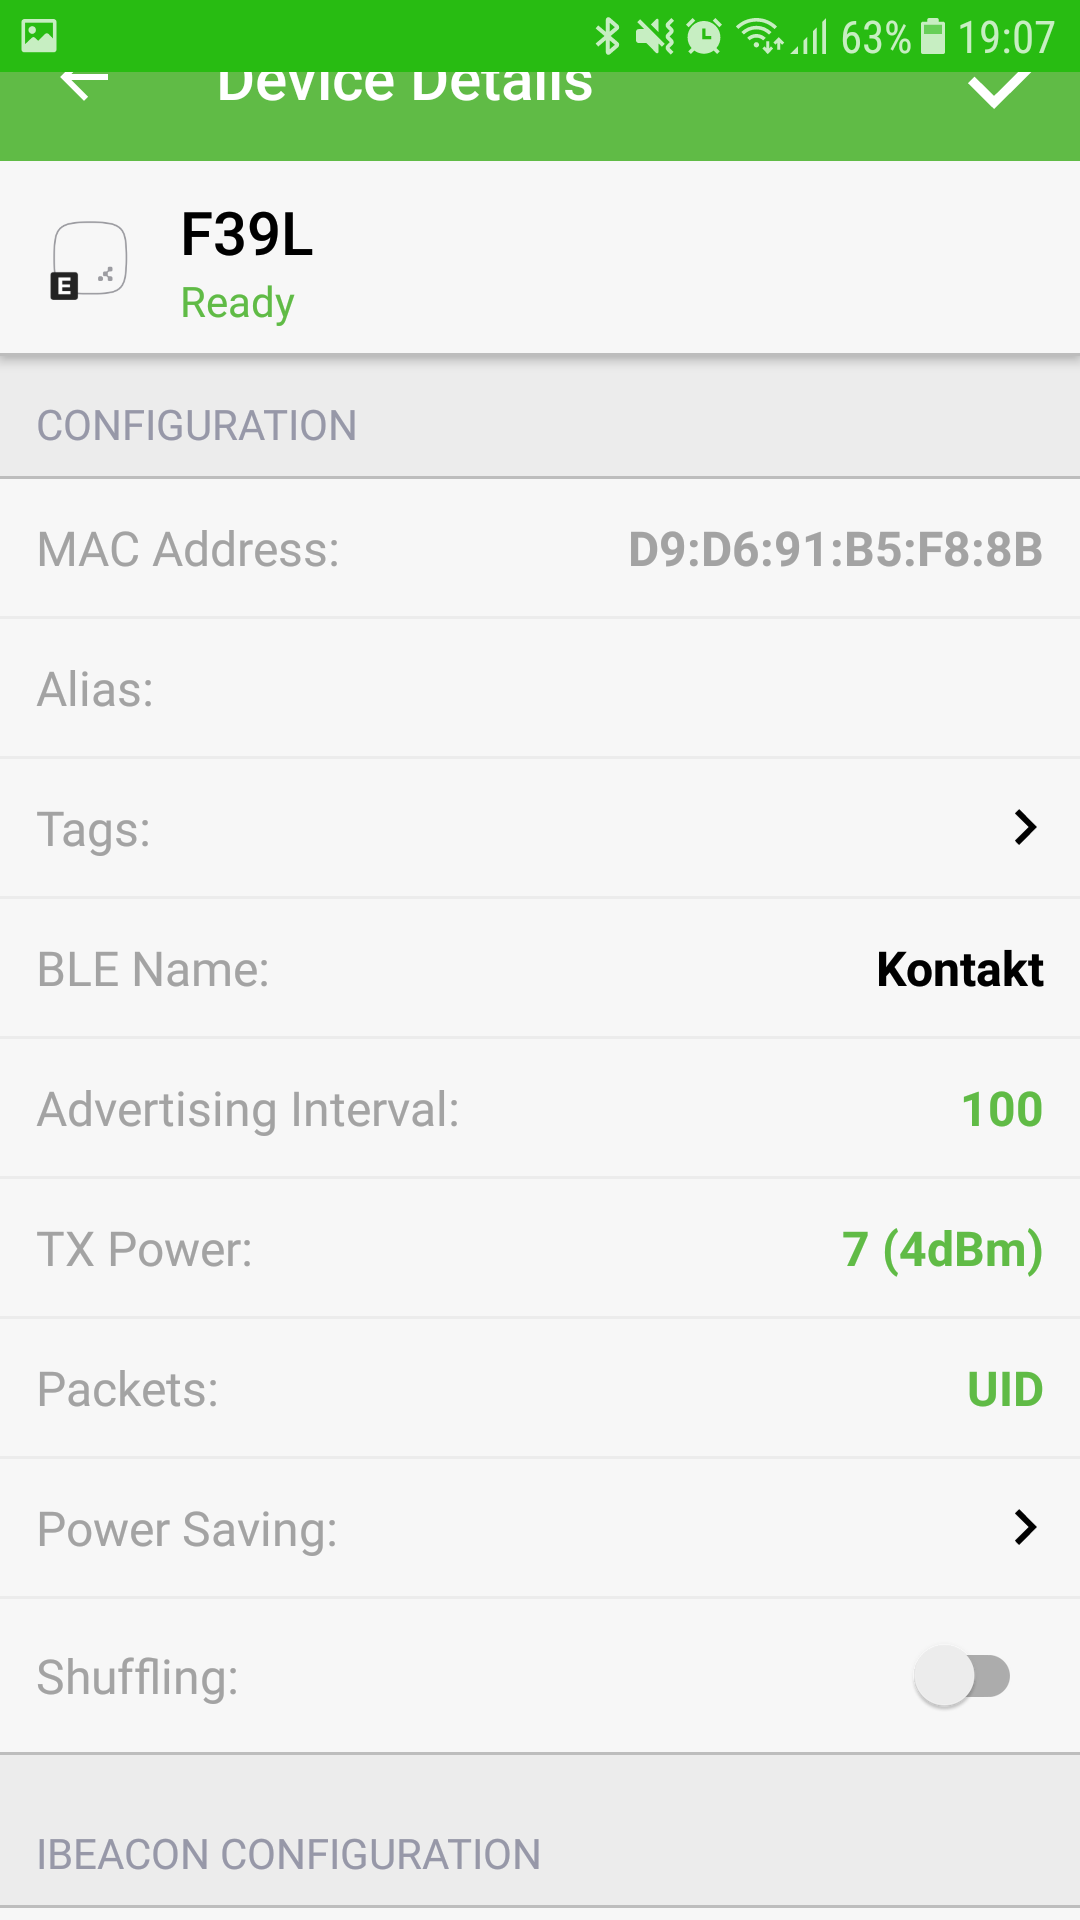
\includegraphics[width=.3\textwidth]{figures/kontaktapp2.png}
\caption[abs]{Configuración que ejemplifica los valores definidos para TX Power y el intervalo de transmisión\\
{\scriptsize (Fuente: Elaboración Propia)}}
\label{fig:kontaktapp2}
\end{figure}

Ademas, los protocolos utilizados son UID de Eddystone por su flexibilidad y transversalidad para los múltiples dispositivos móviles existentes en el mercado.

\section{Lugar de experimentacion}

Para realizar los experimentos, se decide utilizar un lugar en donde las condiciones sean adversas y cambiantes, debido al alto transito de objetos y ademas no se presenten señales GPS. Por lo anterior, se decide utilizar el estacionamiento subterráneo de la universidad Técnica Federico Santa Maria, Campus San Joaquin, ubicado en Vicuña Mackenna 3939. Las dimensiones constan de $144.75m$ de largo y $36m$ de ancho. La \autoref{fig:estSubterraneo} muestra el plano del estacionamiento a escala.

\begin{figure}[ht!]
\centering
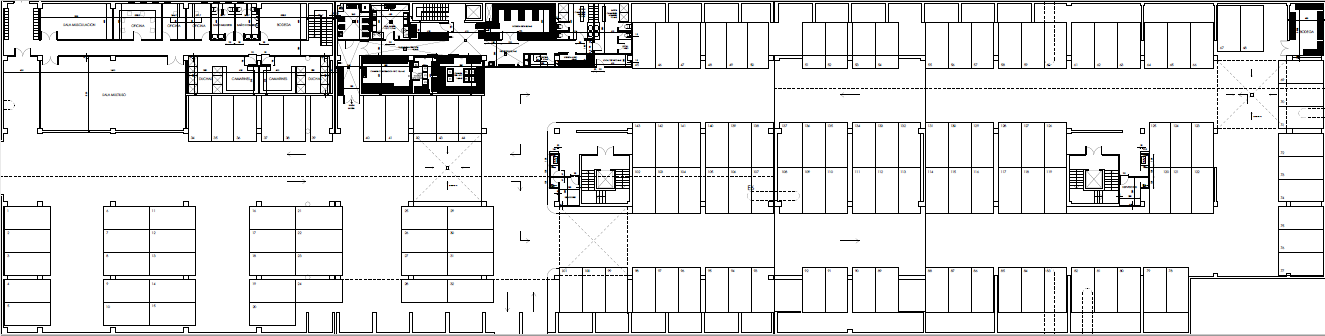
\includegraphics[width=.6\textwidth]{figures/estSubterraneo.png}
\caption[abs]{Plano del estacionamiento subterraneo de la Universidad Federico Santa Maria\\
{\scriptsize (Fuente: Elaboración Propia)}}
\label{fig:estSubterraneo}
\end{figure}

Este lugar es ideal para realizar pruebas, ya que presenta interferencia debido a los vehiculos en transito y la disposicion de los objetos es cambiante. Ademas, se pueden obtener mediciones con ruido producto de la reflexion de las ondas, lo que pone a prueba a los algoritmos de clasificación para detectar estos patrones. 

\begin{figure}[ht!]
\centering
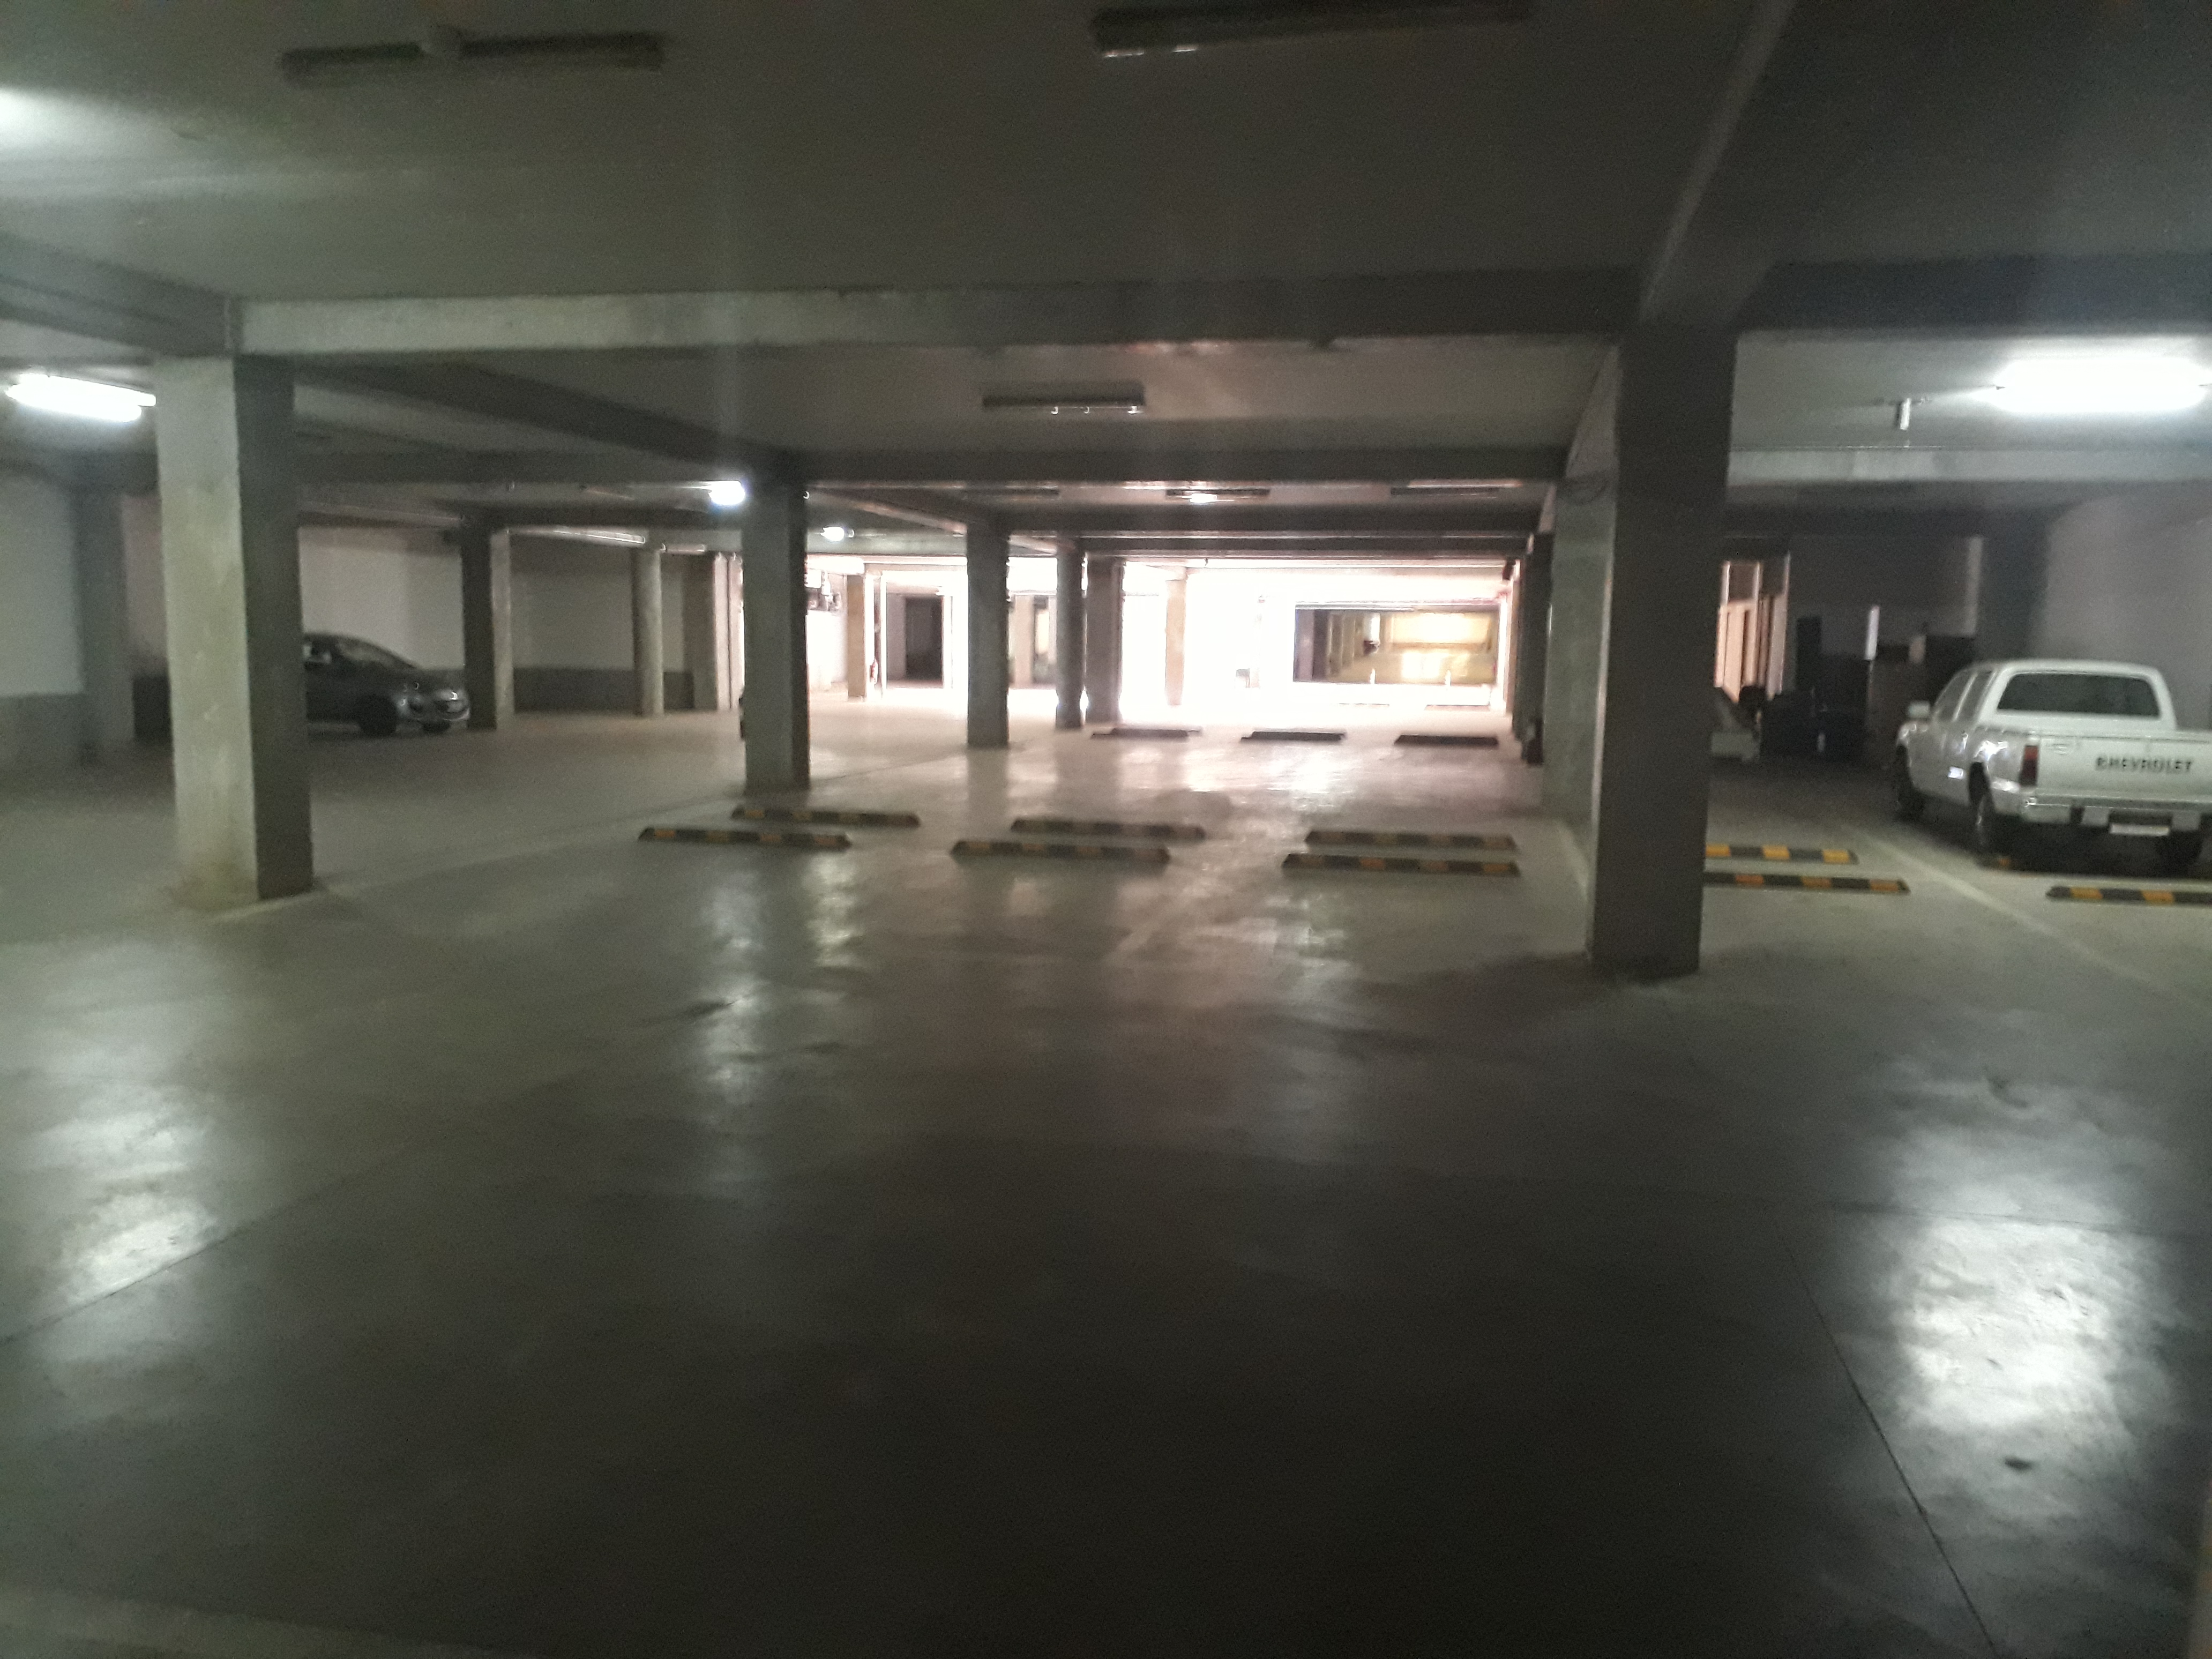
\includegraphics[width=.6\textwidth]{figures/estReal.jpg}
\caption[abs]{Fotografía del espacio de experimentación real, correspondiente al estacionamiento subterraneo\\
{\scriptsize (Fuente: Elaboración Propia)}}
\label{fig:estReal}
\end{figure}


\section{Software Utilizado}

\subsection{Descripción de la aplicación}

La aplicación desarrollada es construida para el sistema operativo Android. Para su desarrollo se utiliza Android Studio \footnote{\url{https://developer.android.com/studio/index.html}}, es IDE oficial para el desarrollo de aplicaciones nativas. El numero de compilación corresponde a $3.0.1$. La selección de este sistema operativo es debido a su fácil acceso y prácticamente ningún costo debido a licencias, ya que es basado en linux por lo que su desarrollo es gratuito, al igual que la distribución de aplicaciones, por lo que es mucho mas efectivo para el desarrollo de una aplicación de prueba bajo un entorno controlado.

Los requisitos básicos de la aplicación construida son los siguientes:

\begin{itemize}
\item Mostrar el plano del lugar de experimentación, el cual funciona como base para posicionar los demás elementos.

\item Permitir la adición de nuevos dispositivos Beacons con su respectivo marcador. Para ello debe detectar automáticamente el beacon mas cercano y sugerir este para su inserción en el mapa.

\item Permitir la captura de datos, es decir, los nuevos fingerprints, en donde el usuario es quien provee la posición exacta y la aplicación mide los valores RSSI durante un periodo de tiempo, para posteriormente almacenarlos en la base de datos. 

\item Modificar los valores de intervalo y el numero de mediciones en cada punto, el cual puede también definirse en periodo de tiempo.

\item Tener una base de datos \textit{SQLite}, la cual permite la persistencia de los datos. También se debe poder transformar esta base de datos a un archivo CSV.

\item Para la etapa online, debe permitir seleccionar el algoritmo a utilizar y mostrar en tiempo real la posición del usuario según el algoritmo usado. Por otra parte, debe guardar estos resultados en un archivo de texto para su posterior análisis.



\end{itemize}

La aplicación construida consta de 3 secciones principales las cuales ayudan a todas las etapas del modelo fingerprint, estas son \textbf{Offline}, \textbf{Online} y \textbf{Configuración}. Estas son descritas a medida que se desarrolla el proceso de la experimentación.


\subsection{scikit-learn}

Para la elaboración de modelos de clasificación, una de las librerías mas utilizadas es scikit-learn o tambien conocida como SKlearn \cite{scikit-learn}, la cual es una completa API para elaborar y realizar maquetas de machine learning. Su core esta basado en python y para su uso se utiliza el siguiente entorno de desarrollo:

\begin{itemize}
\item Anaconda 1.6.2
\item Jupyter Notebook 5.0.0
\item scikit-learn 0.18.2
\item Python 3.6.1
\end{itemize}

Las principales ventajas de utilizar SKlearn son obtener modelos simples y eficientes, que estan muy avanzados y que presentan una comunidad dedicada a su correcto funcionamiento. Ademas esta construida sobre 3 de las librerías mas utilizadas en Python en el contexto de desarrollo científico, como son NumPy, SciPy y Matplotlib. Por otra parte su licencia es de codigo abierto, por lo que cualquiera puede utilizar y modificar el código sin restricciones.

A pesar que en este caso solo se utilizara para los algoritmos de clasificación, PCA y gráficos, también presenta herramientas que agilizan el desarrollo como por ejemplo lectura de archivos, funciones de normalizacion establecidas, funciones de puntuación o accuracy, pre procesamiento de datos, entre otras. También sirve como herramienta de regresión, minería de datos y análisis de datos.

\section{ Tensorflow}

A pesar que SKlearn presenta tantas ventajas para el desarrollo agil de modelos de maquinas de aprendizaje, no es tan bueno en redes neuronales, y no implementa la mayor parte de los algoritmos modernos en este campo. Esto se debe principalmente a que todo el core de SKlearn es python, y se vuelve sumamente lento para entrenar este tipo de redes, sobre todo redes profundas. Para resolver este problema, se decide utilizar Tensorflow \cite{tensorflow2015-whitepaper}, un completo framework de desarrollo de Google, que con respecto a SKlearn es mucho menos intuitivo y de fácil uso al usuario final, ya que su programacion es de mucho mas bajo nivel y requiere conocimiento avanzado de los algoritmos que se quieren implementar.  Mucha veces se describe como las piezas fundamentales para la creacion de algoritmos de maquinas de aprendizaje, como si fueran Legos, no asi SKlearn, el cual ya esta todo listo, solo debe ser utilizados y configurar los parametros de los algoritmos.

Tensorflow es una biblioteca de código abierto y su principal ventaja es que a pesar que la parte superior esta basada en python, esta se comunica internamente a código compilado en C++, lo cual lo vuelve sumamente eficiente. Ademas, por la forma en que Tensorflow representa los datos, es decir, tensores o arreglos multidimensionales, y las operaciones referentes a grafos sin estado que transforman estos tensores, lo vuelve increiblemente rapido para entrenar y desplegar, incluso presenta API para dispositivos moviles en Java, C++ y GO, en donde solo se porta el grafo construido y se puede realizar inferencia en equipos de muy pocos recursos, lo que lo vuelve una alternativa ideal para desarrollar redes neuronales profundas, utilizando  pocos recursos en el sistema operativo Android. A pesar de que presenta operaciones de bajo nivel, igualmente tiene disponible la opcion de API de alto nivel, como por ejemplo implementar redes convolucionales o redes profundas en un par de lineas de codigo Python, conocidos como estimadores de alto nivel.

Finalmente tensorflow basa todo su procesamiento en el grafo computacional mencionado anteriormente, el cual consiste en una serie de operaciones de tensores dispuestos en un grafo de nodos. Luego de que se arma este grafo de operaciones, se puede entrenar mediante las operaciones incluidas en tensorflow, llamados optimizadores, como lo son gradiente descendente. El paso final es utilizar este grafo computacional para probar los modelos y utilizarlos en despliegues reales.


\section{Recolección de fingerprints}


Con todo lo anterior en cuenta, es necesario definir que tipo de dispositivo móvil y sistema operativo se utilizara para colectar los datos en cuestión, que finalmente se transformaran en fingerprint dando lugar al radiomap. En este caso, el dispositivo a utilizar es un dispositivo Samsung Galaxy J7 Prime, que dentro de sus prestaciones posee una CPU Octa-core 1.6 GHz Cortex-A53, una GPU Mali-T830 MP1, 3GB de memoria ram interna y el tipo de Bluetooth corresponde a 4.1 LE. Con respecto a su sitema operativo, es Android 7.0 Nougat el cual no presenta limitaciones en la lectura de las señales Bluetooth por lo que puede recepcionar las señales tan rápido como estas son emitidas.

Definido esto, lo siguiente establecer la forma en que deben ser posicionados los beacons y ademas como funciona la recolección de fingerprints como tal. Para el posicionamiento de los Beacons, se decide utilizar una estrategia de grilla, esto es, ubicarlos de manera equidistante en las esquinas del plano. Ademas, para este trabajo se debe considerar que el plano completo no fue inspeccionado debido a que la densidad de los beacons seria muy baja para lograr óptimos resultados, por lo que finalmente se decide utilizar los 8 beacons en un área reducida del estacionamiento y ubicar cada beacon a una distancia de 16 metros a sus vecinos adyacentes formando esta especie de grilla. Finalmente, el área efectiva a utilizar se calcula según las dimensiones de 16 metros de ancho por 44 metros de largo, con lo que se obtiene un área de $704m^2$. Cabe destacar que un par de beacons fueron ubicados respecto a sus vecinos a una distancia de 12 metros y no 16, debido a la disposición del estacionamiento. 

Con respecto al punto de recolección de fingerprints, se desarrolla una aplicación para el sistema operativo Android, y se decide utilizar una grilla para los puntos de medición o referencia de 4 metros por 4 metros, es decir, cada punto de medición esta en medio de cada celda de esta grilla, consiguiendo de esta manera un total de 44 puntos de referencia. La \autoref{fig:deployBeacons} muestra esta situación.


\begin{figure}[ht!]
\centering
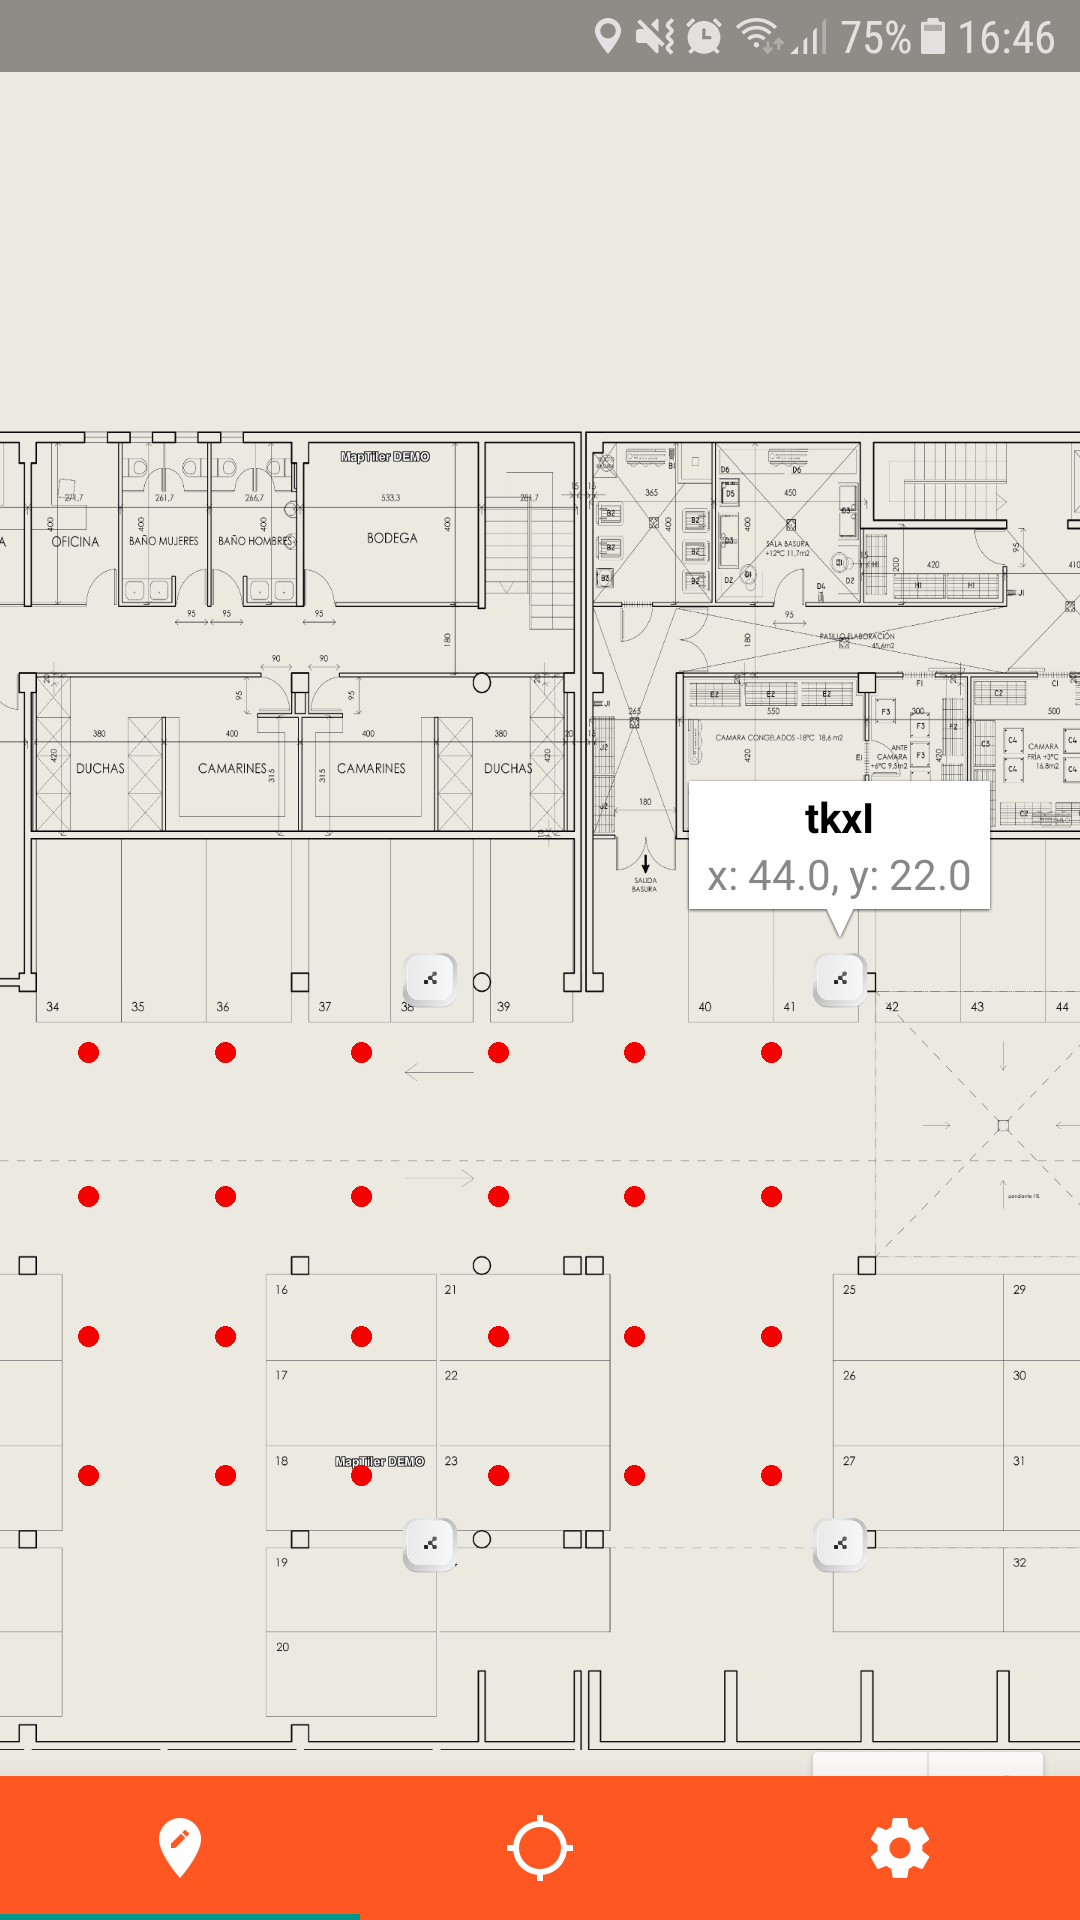
\includegraphics[width=.3\textwidth]{figures/deployBeacons.png}
\caption[abs]{Disposicion de beacons y puntos de referencia dentro de la grilla, utilizando la aplicacion Android\\
{\scriptsize (Fuente: Elaboración Propia)}}
\label{fig:deployBeacons}
\end{figure}

La aplicación consta de una sección offline, en donde se pueden incorporar nuevos Beacons a la base de datos \textit{sqlite}(base de datos por defecto en dispositivos Android), ademas de poner realizar  la captura de datos o fingerprints, definiendo la ubicación actual según algún patrón o posición exacta. Otro punto importante a considerar es el numero de fingerprints a obtener en cada punto de referencia. Considerando el intervalo de emisión de cada Beacon, es necesario establecer un tiempo alto para notar cambios en el lugar de experimentación, por lo que se define una ventana de tiempo de 5 minutos en cada punto de referencia. Sin embargo, para obtener mejores resultados y en vista y considerando que las maquinas de aprendizaje aprenden de mucho mejor manera con datos variados, se decide inspeccionar y recolectar datos a través de diferentes días, con el objetivo de que sea mas fácil para los algoritmos encontrar patrones eventualmente.

Una vez recolectados los datos, se obtiene una base de datos \textit{SQLite} con figerprints, la cual presenta 132000 registros, en donde los dos primeros campos representan la posicion de X y la posicion de Y respectivamente, y los siguientes 8 campos corresponden a los Beacons detectados con su respectiva intensidad de la señal o RSSI. Un punto importante a definir es que valor asignar a los beacons que no han sido detectados, en este caso y como el valor RSSI no puede ser mayor a cero, se decide asignar un valor de 100 dBm como un identificador de que no se ha detectado señal.

Con esta base de datos es posible construir otros tipos de archivos, que resuman todos los fingerprints detectados. Esto se realiza ya que para los algoritmos de machine learning existen muchas mas librerías dedicadas a leer datos en formatos mas convencionales como TXT o CSV. Por lo mismo, en la aplicación se define una sección de configuración para transformar y almacenar esta base de datos en formato CSV o \textit{comma-separated values}.  La \autoref{fig:configApp} muestra esta pestaña de configuracion, incluyendo el numero de mediciones y las opciones de exportar la base de datos, transformarla a CSV o eliminarla.

\begin{figure}[ht!]
\centering
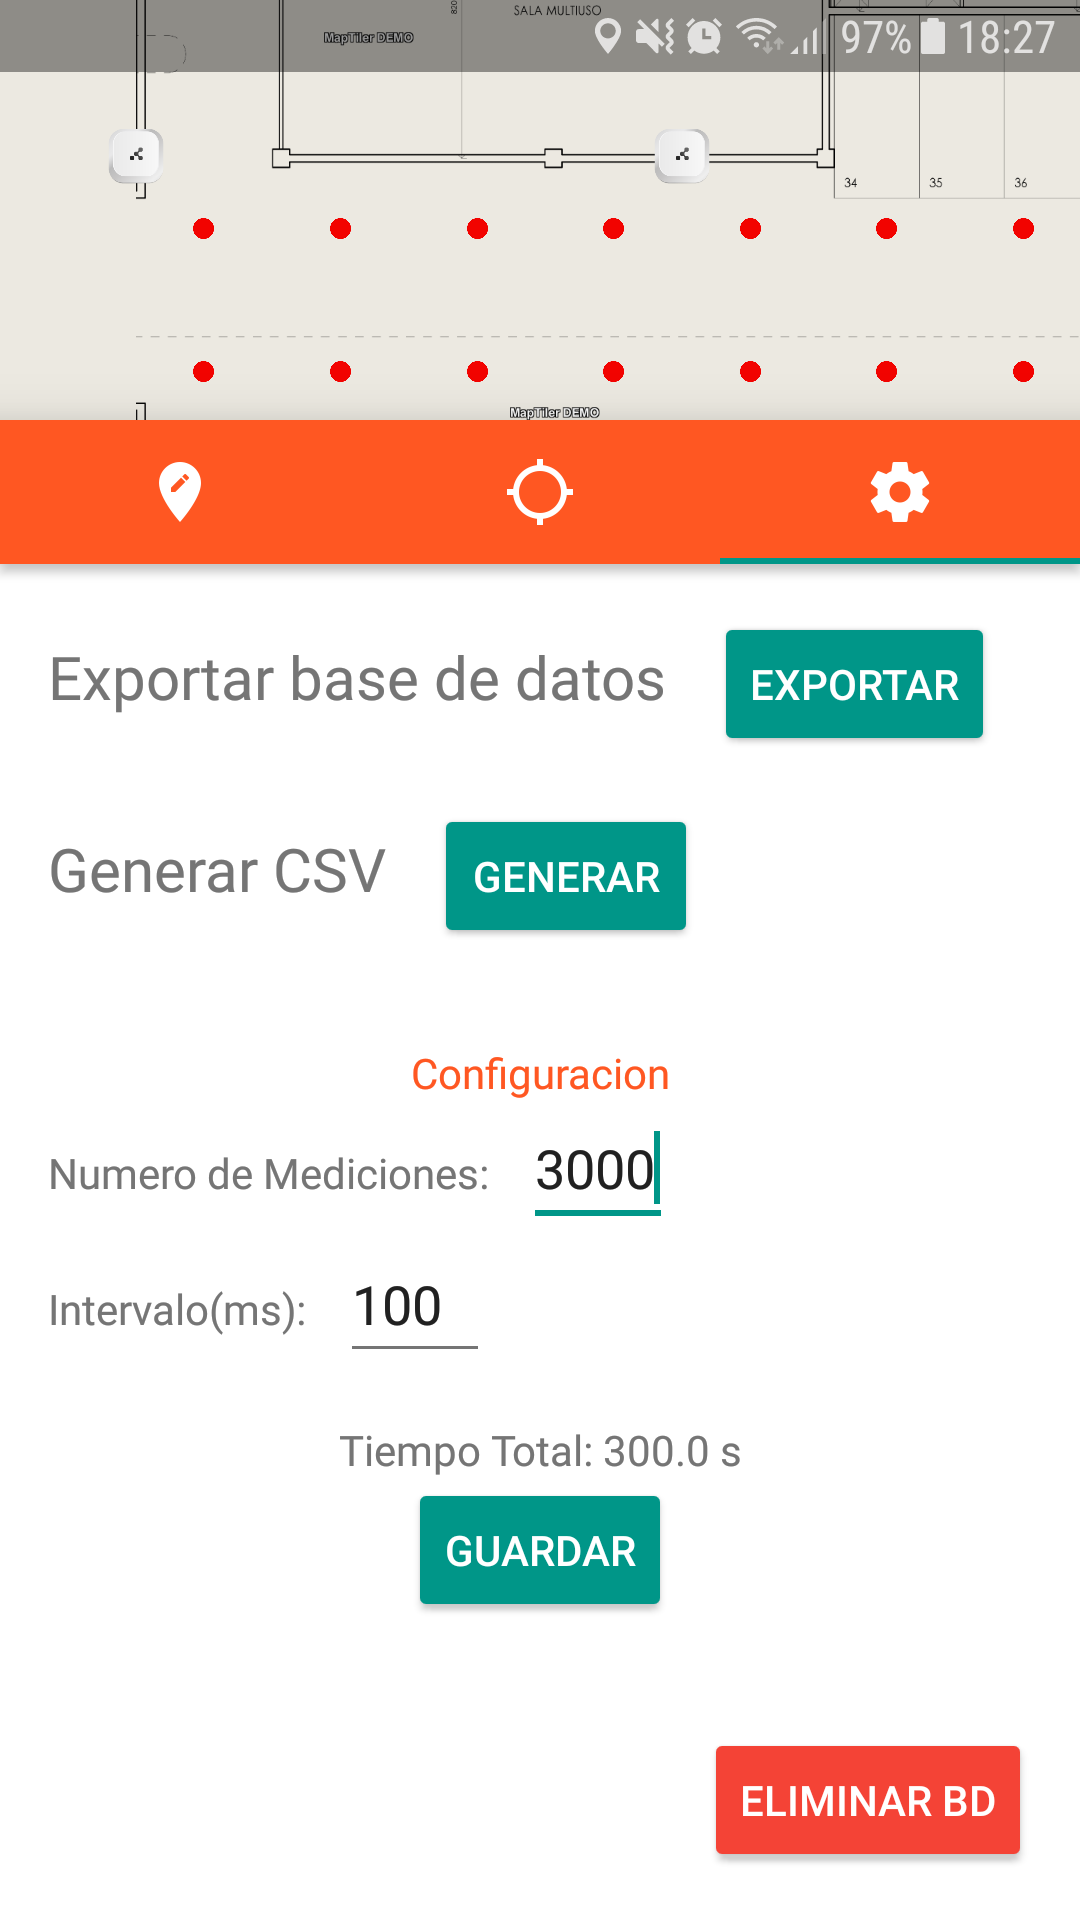
\includegraphics[width=.3\textwidth]{figures/configApp.png}
\caption[abs]{Pestaña de configuración de la aplicación Android, donde se puede configurar el tiempo y exportar la base de datos a CSV\\
{\scriptsize (Fuente: Elaboración Propia)}}
\label{fig:configApp}
\end{figure}


Un ejemplo del archivo CSV obtenido se presenta en la \autoref{fig:ejemploCSV}


\begin{figure}[ht!]
\centering
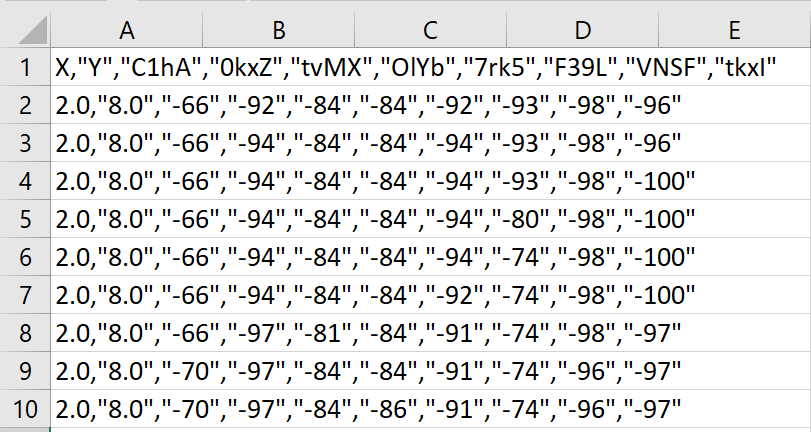
\includegraphics[width=.6\textwidth]{figures/ejemplo_csv.png}
\caption[abs]{Segmento del archivo CSV obtenido a partir de la base de datos. Los primeros dos registros corresponden a las coordenadas y los siguientes, los id unicos de cada Beacon utilizado, con su respectivo en dBm en cada fingerprint. \\
{\scriptsize (Fuente: Elaboración Propia)}}
\label{fig:ejemploCSV}
\end{figure}

Todos estos pasos de recolección son necesarios para los posteriores análisis y entrenamiento de los algoritmos de maquinas de aprendizaje. Para entrenar los clasificadores, se considera entonces cada Beacon en un registro como un feature, es decir, un atributo que funcionara como predictoria para la clasificación. Las etiquetas de cada registro puede corresponder tanto a $X$ como a $Y$, entonces debe entrenarse en ambos casos, por lo que cada clasificador debe presentar 4 casos, esto es $X$ e $Y$ con PCA y $X$ e $Y$ solo con normalizacion de los datos.


\section{Visualizacion de los datos obtenidos}

En maquinas de aprendizaje, siempre es bueno analizar los datos para determinar patrones o el comportamiento general de los datos. Claramente no es posible visualizar todas las características de una vez, ya 	que al ser mas de tres dimensiones, es complejo para la visualización humana. Mientras los datos en dos o tres  dimensiones pueden ser graficados e interpretados, los datasets de altas dimensiones no cuentan con la misma suerte, y ellos representan la mayor parte de los problemas existentes. El fin de determinar la estructura de los datos es reconocer por ejemplo algún comportamiento extraño o ruido, el cual posteriormente puede ser removido en el caso de ser necesario. Para permitir la visualización de la estructura del dataset, la dimension debe ser reducida de alguna manera, para ser representada en un plano o el espacio cartesiano, algo que es muy intuitivo a la visualización humana.

Para sobrellevar esto, la manera mas simple es tomar una proyección aleatoria de los datos, es decir, seleccionar los features mas representativos según alguna especie de peso o ranking. Esto permite algún grado de visualización de la estructura de los datos, pero se pierde información que muchas veces puede ser relevante. En este tipo de proyecciones, la estructura mas interesante de los datos se pierde debido a la falta de información, por lo que no se representa el problema completo.

Ademas, existen muchos algoritmos tanto supervisados como no supervisados, que son lineales y permiten la reducción de la dimensionalidad, como son \textbf{PCA},  análisis de componentes independientes, analisis de discriminante lineal(\textbf{LDA}), entre otros. En este trabajo PCA es utilizado para reducir la dimensionalidad y evitar la correlación lineal entre los features de los datos. Estos algoritmos definen formas de realizar proyecciones lineales interesantes de los datos. Aunque estos metodos son frecuentemente utilizados, es importante ademas definir otro tipo de algoritmos que ayuden a establecer si entre todas las variables existen estructuras no lineales.

Para conseguir esto, a continuacion se utilizan tecnicas de \textbf{Manifold Learning}, las cuales pueden generalizar los frameworks lineales como PCA para ser sensibles a datos altamente no lineales. Un punto importante a destacar es que la mayor cantidad de algoritmos de este tipo son no supervisados, por lo que pueden encontrar las clases automaticamente y separarlas a partir de los mismos datos, sin necesidad de suministrar las etiquetas de cada fingerprint.

Los algoritmos a comparar no seran abordados en detalle porque no es el objetivo de este trabajo, solo se analizaran sus resultados respectivos. Los algoritmos utilizados son Locally Linear Embedding de tipo standar, ltsa, hessian y modificado. Ademas se utilizan otros tres metodos correspondientes a Isomap, \textit{Multi-dimensional Scaling}, \textit{Spectral Embedding} y finalmente \textit{t-distributed Stochastic Neighbor Embedding}(\textbf{t-SNE}). Para utilizar estos metodos en primer lugar se normalizan los datos mediante SKlearn, dejándolos con media igual a cero y varianza unitaria, es decir, datos normalmente distribuidos como se define a continuación:


\section{Entrenamiento de clasificadores}

Para el entrenamiento de los clasificadores, se debe tener en cuenta como se menciona anteriormente, que para la gran mayoría de los algoritmos es necesario una normalizacion previa. Esto es particularmente importante en problemas en donde cada atributo puede diferir mucho en orden de magnitud con otras variables. En este caso, no es ciertamente un requisito, ya que los atributos poseen valores de la misma magnitud, porque todas reflejan valores en dBm en un mismo rango, sin embargo igualmente es una buena practica para algoritmos basados en distancia como KNN o SVM, sobre todo por la inclusión del valor 100dbm incorporado para denotar la ausencia de un dispositivo Beacon.

Antes de comenzar con el entrenamiento en si, es bueno realizar un analisis de los datos, es decir, xddd
\chapter{Resultados}

\section{Métricas Obtenidas}

Para los resultados, se deben elaborar métricas que permitan determinar cuáles fueron los mejores algoritmos, es decir, los que presentan mejor desempeño según la experimentación determinada anteriormente. Primero se construyen las tablas que muestran los valores más relevantes en primera instancia, es decir, los errores en cada eje coordenado, sus promedios de error, varianzas y finalmente el \textit{root squared mean error}, o error cuadrático medio, el cual en términos euclidianos, representa la distancia de un punto a otro. La fórmula de este último es:

\begin{equation}
RMSE = \sqrt{\frac{1}{n} \sum_{j=1}^{n}(y_{j} - \hat{y_{j}})^{2}} 
\end{equation}

Para las tablas se considera el método dinámico y estático definido anteriormente. La primera tabla muestra los resultados obtenidos en el método dinámico sin utilizar PCA. Se debe considerar que todos los valores están en metros.


\begin{table}[ht!]
\centering
\caption[Resultados método dinámico sin  utilizar PCA]{Resultados método dinámico sin  utilizar PCA}
\label{tabla-dinamica-nPCA}
\begin{tabular}{|c|c|c|c|c|c|}
\hline
Clasificador & Error x & Error y & Varianza x & Varianza y & RMSE    \\ \hline
KNN          & 1.5858  & 4.6391  & 7.1970     & 2.1780     & 6.9323  \\ \hline
SVM          & 6.8207  & 2.8874  & 1.7243     & 0.5989     & 10.0323 \\ \hline
NN           & 4.3784  & 3.9113  & 13.0950    & 5.0712     & 8.2994  \\ \hline
\end{tabular}
\end{table}


Como muestra la \autoref{tabla-dinamica-nPCA}, los mejores resultados en términos generales son obtenidos por el método KNN, ya que los promedios en general son bajos, así como el RMSE. A pesar de esto, se debe notar que lo sigue Neural Network con un RMSE promedio de 8.2994 metros. 

La \autoref{tabla-dinamico-pca} muestra los resultados obtenidos por el método dinámico utilizando PCA.

\begin{table}[!ht]
\centering
\caption[Resultados método dinámico utilizando PCA con 5 componentes]{Resultados método dinámico utilizando PCA con 5 componentes}
\label{tabla-dinamico-pca}
\begin{tabular}{|c|c|c|c|c|c|}
\hline
Clasificador & Error x & Error y & Varianza x & Varianza y & RMSE   \\ \hline
KNN PCA      & 2.0023  & 4.3983  & 7.5113     & 2.0696     & 6.6812 \\ \hline
SVM PCA      & 6.8948  & 2.4257  & 4.1134     & 2.0348     & 9.5668 \\ \hline
NN PCA       & 5.8874  & 4.4513  & 8.6088     & 3.2089     & 9.5188 \\ \hline
\end{tabular}
\end{table}

En este caso, los resultados son ligeramente mejores en términos de RMSE, lo cual indica que PCA si puede eliminar parte de la correlación espacial e información repetida dentro de los datos. En este caso nuevamente KNN con PCA obtiene el mejor resultado, seguido por Neural Network y finalmente SVM. Las varianzas de cada eje igualmente son relativamente altas, por lo que esto puede afectar mucho el posicionamiento en general, ya que, a mayor varianza, más error durante el tiempo se presenta, y más alejados están los valores desde el promedio.

Para la siguiente tabla, ahora se considera el método estático, el cual como se ha descrito, mide la posición al estar estático en un determinado lugar. 

\begin{table}[!h]
\centering
\caption[Resultados método estático sin utilizar PCA]{Resultados método estático sin utilizar PCA}
\label{tabla-estatica}
\begin{tabular}{|c|c|c|c|c|c|}
\hline
Clasificador & Error x & Error y & Varianza x & Varianza y & RMSE   \\ \hline
KNN          & 3.2385  & 1.5417  & 3.3321     & 1.0940     & 5.0520 \\ \hline
SVM          & 5.2493  & 1.6986  & 2.0598     & 0.7594     & 7.0241 \\ \hline
NN           & 3.7300  & 2.1937  & 5.8885     & 0.7373     & 4.4857 \\ \hline
\end{tabular}
\end{table}

Para este caso, la \autoref{tabla-estatica}, muestra que ahora los mejores resultados son obtenidos por el método Neural Networks con un RMSE de 4.4857 en promedio. Para todos los algoritmos, las varianzas se ven reducidas sustancialmente, lo que es esperable debido a que, al estar estático en una posición, las ondas electromagnéticas no se ven alteradas o cambiantes a través del tiempo, lo cual estabiliza la señal recibida por los Beacons. Para este caso, primero es NN, luego KNN y finalmente SVM en términos de RMSE. Igualmente, los valores de error obtenidos son muy altos para lograr un posicionamiento exacto.

Por último, las métricas obtenidas para el posicionamiento estático utilizando PCA se muestran a continuación.

\begin{table}[!h]
\centering
\caption[Resultados método estático utilizando PCA con 5 componentes]{Resultados método estático utilizando PCA con 5 componentes}
\label{estatico-pca}
\begin{tabular}{|c|c|c|c|c|c|}
\hline
Clasificador & Error x & Error y & Varianza x & Varianza y & RMSE   \\ \hline
KNN PCA      & 2.9892  & 1.4475  & 3.1487     & 1.6391     & 5.0340 \\ \hline
SVM PCA      & 3.2313  & 1.4905  & 3.0630     & 1.7817     & 5.1757 \\ \hline
NN PCA       & 1.5578  & 1.7488  & 3.8045    & 2.6885     & 3.9341 \\ \hline
\end{tabular}
\end{table}
 
La \autoref{estatico-pca} muestra mejores resultados para todos los clasificadores, disminuyendo así los valores totales. Esto muestra nuevamente que mediante la técnica PCA es posible reducir el error. Por otra parte, las varianzas permanecen pequeñas a excepción de Neural Network. El mejor resultado es obtenido por Neural Network con PCA con un error promedio de 3.9341 metros, seguido por KNN PCA y finalmente SVM PCA.

El siguiente análisis realizado, tiene que ver con el valor de \textit{Cumulative distribution function}, el cual está definido como el valor de una variable aleatoria $X$, o su función de distribución, que al ser evaluada en $x$, es la probabilidad que $X$ tome valores menores o iguales a $x$, Esta función está definida matemáticamente como:

\begin{equation}
F_{X} (x) = P(X \le x)
\end{equation}

La importancia de este indicador es que refleja en este caso, que tan frecuente se repite un valor de error, o, dicho de otra forma, en qué porcentaje se puede asegurar que el error será menor o igual a un determinado valor, por ejemplo el 90\% de las veces el error es menor a 10 metros. Con esta definición, a continuación, se procede a mostrar los gráficos obtenidos tanto para el método estático como para el método dinámico.

\begin{figure}[ht!]
\centering
\begin{subfigure}{.5\textwidth}
  \centering
  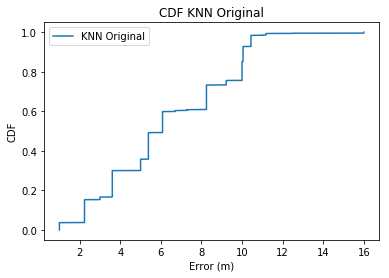
\includegraphics[width=.8\linewidth]{figures/cdf-knn-dinamico.png}
  \caption{CDF KNN}
  \label{fig:sub1}
\end{subfigure}%
\begin{subfigure}{.5\textwidth}
  \centering
  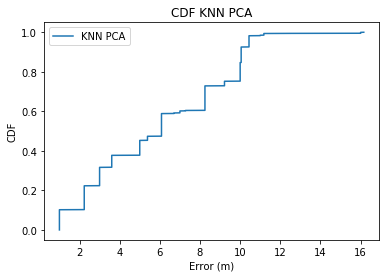
\includegraphics[width=.8\linewidth]{figures/cdf-knnPCA-dinamico.png}
  \caption{CDF KNN PCA}
  \label{fig:sub2}
\end{subfigure}

\begin{subfigure}{.5\textwidth}
  \centering
  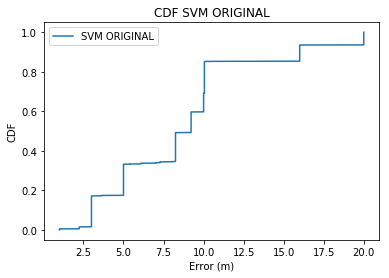
\includegraphics[width=.8\linewidth]{figures/cdf-svm-dinamico.png}
  \caption{CDF SVM}
  \label{fig:sub1}
\end{subfigure}%
\begin{subfigure}{.5\textwidth}
  \centering
  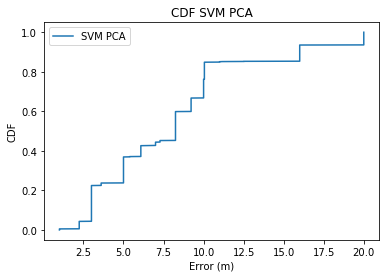
\includegraphics[width=.8\linewidth]{figures/cdf-svmPCA-dinamico.png}
  \caption{CDF SVM PCA}
  \label{fig:sub2}
\end{subfigure}

\begin{subfigure}{.5\textwidth}
  \centering
  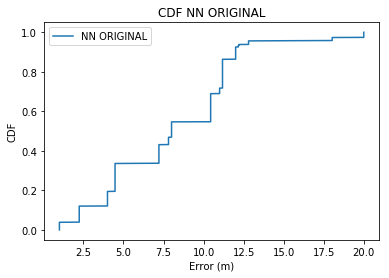
\includegraphics[width=.8\linewidth]{figures/cdf-nn-dinamico.png}
  \caption{CDF NN}
  \label{fig:sub1}
\end{subfigure}%
\begin{subfigure}{.5\textwidth}
  \centering
  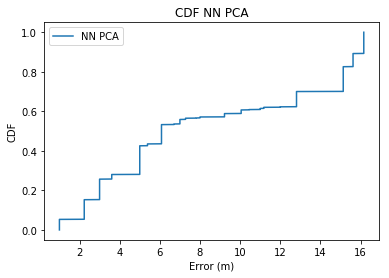
\includegraphics[width=.8\linewidth]{figures/cdf-nnPCA-dinamico.png}
  \caption{CDF NN PCA}
  \label{fig:sub2}
\end{subfigure}
\caption[Cummulative distribution function para el método dinámico]{Cummulative distribution function para el método dinámico obtenido utilizando los distintos algoritmos \\
{\scriptsize (Fuente: Elaboración Propia)}}
\label{fig:cdf-dinamicos}
\end{figure}

Los gráficos muestran que los valores son muy símiles en cuanto a si se utiliza PCA o no. K-NN se mantiene el 80\% de las veces bajo los 10 metros, en ambos casos y cerca del 40\% bajo los 4 metros. Por otro lado, SVM igualmente el 80\% de las veces está bajo los 10 metros con respecto a SVM sin utilizar PCA, el 40\% de las veces está bajo los 8 metros y utilizando PCA esto ocurre el 60\% de las veces por lo que PCA es más estable en este sentido, y genera valores más uniformes. Finalmente, con las redes neuronales, los resultados presentados sin utilizar PCA, el 80\% de las veces esta cercano a los 12 metros y 50\% de las veces en los 7.5 metros. Utilizando PCA en este último caso, los resultados son mejores para porcentajes más bajos, ya que el 80\% de las veces esta sobre los 15 metros aproximadamente,  pero esto no cambia relativamente hacia porcentajes superiores, sin embargo para porcentajes inferiores los valores mejoran, ya que por ejemplo para un error menor a 6 metros, ocurre con una probabilidad del 60\% .

Para ver el mínimo error al 100\%, es decir, el error mínimo que está asegurado, se realiza la siguiente tabla comparando sus valores utilizando o no PCA. Nuevamente los valores están en metros.

\begin{table}[!h]
\centering
\caption[Error con un CDF del 100 \% para los algoritmos analizados  en el método dinámico]{Error con un CDF del 100 \% para los algoritmos analizados  en el método dinámico}
\label{cambio-cdf-dinamico}
\begin{tabular}{|c|c|c|c|}
\hline
Clasificador & Sin PCA & Con PCA & Mejora     \\ \hline
KNN          & 16.576  & 16.1554 & 2.5374 \%  \\ \hline
SVM          & 20.8962 & 19.3874 & 7.2204 \%  \\ \hline
NN           & 20.5677 & 16.1554 & 21.4525 \% \\ \hline
\end{tabular}
\end{table}


Como se observa en la tabla \autoref{cambio-cdf-dinamico}, todos los valores son mejorados utilizando PCA, además los errores menores se obtienen con NN y KNN, aunque KNN es más estable ya que con y sin PCA presenta valores semejantes.

Para el método estático se realiza el mismo análisis. Los gráficos obtenidos para el error CDF son los siguientes:

\begin{figure}[ht!]
\centering
\begin{subfigure}{.5\textwidth}
  \centering
  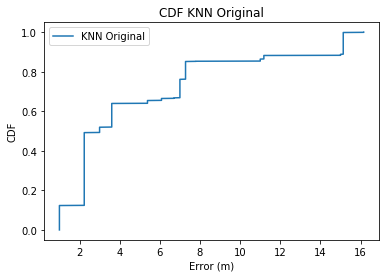
\includegraphics[width=.8\linewidth]{figures/cdf-knn-estatico.png}
  \caption{CDF KNN}
  \label{fig:sub1}
\end{subfigure}%
\begin{subfigure}{.5\textwidth}
  \centering
  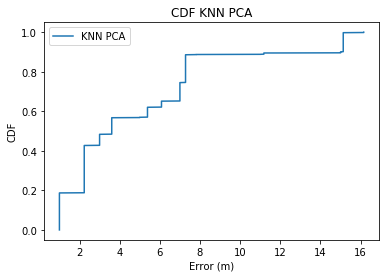
\includegraphics[width=.8\linewidth]{figures/cdf-knnPCA-estatico.png}
  \caption{CDF KNN PCA}
  \label{fig:sub2}
\end{subfigure}

\begin{subfigure}{.5\textwidth}
  \centering
  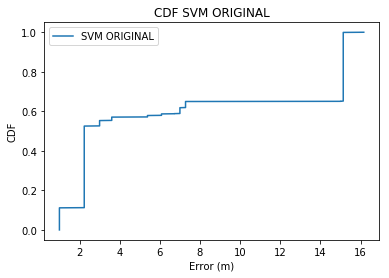
\includegraphics[width=.8\linewidth]{figures/cdf-svm-estatico.png}
  \caption{CDF SVM}
  \label{fig:sub1}
\end{subfigure}%
\begin{subfigure}{.5\textwidth}
  \centering
  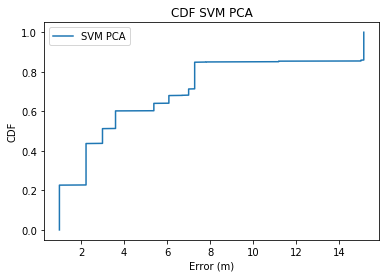
\includegraphics[width=.8\linewidth]{figures/cdf-svmPCA-estatico.png}
  \caption{CDF SVM PCA}
  \label{fig:sub2}
\end{subfigure}

\begin{subfigure}{.5\textwidth}
  \centering
  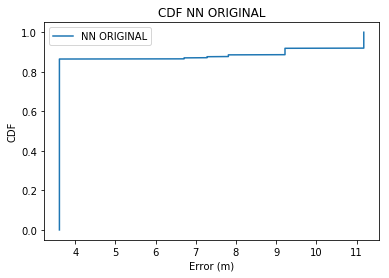
\includegraphics[width=.8\linewidth]{figures/cdf-nn-estatico.png}
  \caption{CDF NN}
  \label{fig:sub1}
\end{subfigure}%
\begin{subfigure}{.5\textwidth}
  \centering
  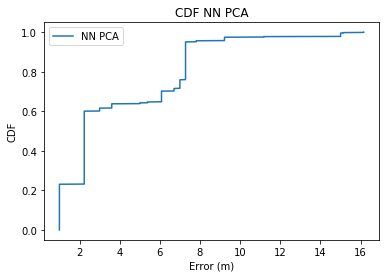
\includegraphics[width=.8\linewidth]{figures/cdf-nnPCA-estatico.png}
  \caption{CDF NN PCA}
  \label{fig:sub2}
\end{subfigure}
\caption[Cummulative distribution function para el método estático]{Cummulative distribution function para el método estático obtenido utilizando los distintos algoritmos \\
{\scriptsize (Fuente: Elaboración Propia)}}
\label{fig:cdf-estaticos}
\end{figure}

Los gráficos para los casos estáticos muestran de manera general que los resultados son mucho mejores, esto es esperable debido a como se discute anteriormente, al estar estático es mucho más estable la señal y por ello se obtienen mejores valores de CDF. Para KNN, el error a los 8 metros se mantiene con una probabilidad de sobre el 80\%, lo cual representa una mejora aproximada de 2 metros respecto al método dinámico. Utilizando PCA se mantiene la tendencia, además se debe observar que para un error menor o igual a 4 metros, ocurre con probabilidad de 60\% lo cual es una mejora significativa.

Para SVM, aunque el error es muy grande en general, se debe tener en cuenta que con cerca del 50\% de las veces, el error esta cercano a los 2 metros. Para SVM con PCA los resultados son muy similares al método dinámico. Finalmente, para las redes neuronales, ocurre un comportamiento distinto a los anteriormente vistos, ya que la probabilidad de que el error sea menor o igual a 2 metros sobrepasa el 80\%, es decir esta siempre muy cercano a la posición verdadera. Esto indica que NN estático es muy estable, a diferencia de lo que ocurre con este mismo algoritmo en el método dinámico. Con respecto a NN con PCA, es claro que no existe mejora con respecto al caso sin PCA, de hecho, empeora el desempeño. Esto puede deberse a factores que serán explicados posteriormente, con respecto a las propiedades de las redes neuronales. Lo que se debe tener en cuenta es que la probabilidad de un error menor a 8 metros es cercana al 90\%, y el 60\% de las veces el error es menor a 2 metros, para NN con PCA.

La tabla del error mínimo al 100\% de CDF se muestra a continuación:

\begin{table}[!h]
\centering
\caption[Error con un CDF del 100 \% para los algoritmos analizados  en el método estático]{Error con un CDF del 100 \% para los algoritmos analizados  en el método estático}
\label{cambio-cdf-estatico}
\begin{tabular}{|c|c|c|c|}
\hline
Clasificador & Sin PCA  & Con PCA & Cambio    \\ \hline
KNN          & 16.1554  & 16.1554 & 0 \%      \\ \hline
SVM          & 16.1554  & 15.1327 & 6.33 \%   \\ \hline
NN           & 11.18033 & 16.1554 & -44.49 \% \\ \hline
\end{tabular}
\end{table}

Los cambios para KNN y SVM no son significativos, y además los errores mínimos son muy similares, del orden de los 16 metros, lo cual indica que PCA funciona efectivamente para reducir la información redundante. Con respecto a NN, se presenta una anomalía al utilizar o no PCA, esto se debe a que las redes neuronales ya hacen una reducción de la dimensionalidad en sus capas escondidas, y retienen lo mejor de la información en cada paso, por lo que aplicar PCA no ayuda demasiado, debido a que resta información relevante, entonces, para Neural Networks, específicamente deep learning, PCA no es efectivo, y es mejor pasar la mayor cantidad de información \textbf{relevante} que se posea.

El siguiente análisis tiene relación con la dispersión del error, vale decir, que tan distintos son los valores, y además determinar en qué valores se agrupan en su mayoría los datos. Para ello se utiliza un análisis de diagrama de cajas o \textit{boxplot}. Con este tipo de análisis se puede visualizar la dispersión y distribución de los datos en términos de cuartiles. En primer lugar, se construyen las siguientes tablas que muestran los valores relevantes para el boxplot. La primera tabla resume los valores de error obtenidos para el método dinámico.

\begin{table}[!ht]
\centering
\caption[Tabla Boxplot método dinámico]{Tabla resumen de los valores necesarios obtenidos para construir el Boxplot del método dinámico}
\label{tabla-boxplot-dinamico}
\begin{tabular}{|c|c|c|c|c|c|c|c|c|}
\hline
\textbf{Clasificador} & \textbf{Mediana} & \textbf{25\%} & \textbf{75\%} & \textbf{90\%} & \textbf{95\%} & \textbf{IQR} & \textbf{Min} & \textbf{Max} \\ \hline
KNN                   & 6.0827           & 3.6055        & 9.2195        & 10.0498       & 10.4403       & 5.6139       & 0.0            & 16           \\ \hline
KNN PCA               & 6.0827           & 3.0           & 9.2195        & 10.0498       & 10.4403       & 6.2195       & 0.0          & 16.1554      \\ \hline
SVM                   & 9.2195           & 5.0           & 10.0498       & 16.0          & 20.0          & 5.0498       & 0.0          & 16.0         \\ \hline
SVM PCA               & 8.2462           & 5.0           & 10.0          & 16.0          & 20.0          & 5.0          & 0.0          & 16.0         \\ \hline
NN                    & 8.0              & 4.4721        & 11.1803       & 12.0          & 12.8062       & 6.7082       & 0.0          & 20.0         \\ \hline
NN PCA                & 6.0827           & 3.0           & 15.1327       & 16.1554       & 16.1554       & 12.1327      & 0.0          & 16.1554      \\ \hline
\end{tabular}
\end{table}


Para el método estático, la \autoref{tabla-boxplot-estatico} muestra los valores resultantes de error.

\begin{table}[!ht]
\centering
\caption[Tabla Boxplot método estático]{Tabla resumen de los valores necesarios obtenidos para construir el Boxplot del método estático}
\label{tabla-boxplot-estatico}
\begin{tabular}{|c|c|c|c|c|c|c|c|c|}
\hline
\textbf{Clasificador} & \textbf{Mediana} & \textbf{25\%} & \textbf{75\%} & \textbf{90\%} & \textbf{95\%} & \textbf{IQR} & \textbf{Min} & \textbf{Max} \\ \hline
KNN                   & 3.0              & 2.2360        & 7.0           & 15.1327       & 15.1327       & 4.7639       & 0.0          & 11.1803      \\ \hline
KNN PCA               & 3.6055           & 2.2360        & 7.2801        & 15.0          & 15.1327       & 5.0440       & 0.0          & 11.1803      \\ \hline
SVM                   & 2.2360           & 2.1604        & 15.1327       & 15.1327       & 15.1327       & 12.9723      & 0.0          & 16.1554      \\ \hline
SVM PCA               & 3.0              & 2.1604        & 7.2801        & 15.1327       & 15.1327       & 5.1197      & 0.0          & 11.1803      \\ \hline
NN                    & 3.6055           & 3.6055        & 3.6055        & 9.2195        & 11.1803       & 0.0          & 3.6055       & 3.6055       \\ \hline
NN PCA                & 2.2360           & 2.4053        & 7.0           & 7.2801        & 7.2801        & 4.7639       & 0.0          & 11.1803      \\ \hline
\end{tabular}
\end{table}

Finalmente, el diagrama de cajas es el siguiente:

\begin{figure}[ht!]
\centering
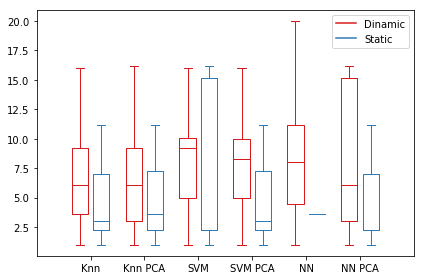
\includegraphics[width=.6\textwidth]{figures/boxplot.png}
\caption[Diagrama de cajas para método estático y dinámico]{Diagrama de cajas para método estático y dinámico \\
{\scriptsize (Fuente: Elaboración Propia)}}
\label{fig:boxplot}
\end{figure}

La \ref{tabla-boxplot-dinamico} y \ref{tabla-boxplot-estatico} muestran los valores resultantes. Se debe tener en cuenta que los valores son iguales o muy similares cuando se utiliza PCA con el algoritmo original, debido a que la distribución de los datos es idéntica y el algoritmo es el mismo, además como se menciona anteriormente, los valores no cambian significativamente lo cual hace que PCA mantenga la distribución original y no cambie demasiado sus valores.

Se debe notar que muchas veces se repiten los valores de mediana o los cuartiles, por ejemplo, entre distintos algoritmos, sobre todo para el método estático. Esto puede deberse a la gran cantidad de datos.

Por último, antes de analizar en términos generales los resultados, se procede a mostrar las diferencias temporales existentes, es decir, los incrementos referentes a la técnica PCA. La \autoref{tiempo-tabla} muestra estos resultados en términos de milisegundos y la respectiva mejora.


\begin{table}[ht!]
\centering
\caption[Mejoras de tiempo en cada algoritmo]{Mejoras de tiempo en cada algoritmo al usar la técnica PCA para reducir la dimensionalidad}
\label{tiempo-tabla}
\begin{tabular}{|c|c|c|c|}
\hline
\textbf{Clasificador} & \textbf{Sin PCA} & \textbf{Con PCA} & \textbf{Incremento} \\ \hline
KNN                   & 64.9642          & 59.6786          & 8.1361\%            \\ \hline
SVM                   & 54.5985          & 25.6085          & 53.0966\%           \\ \hline
NN                    & 0.7610           & 0.5777           & 24.0867\%           \\ \hline
\end{tabular}
\end{table}



\section{Análisis de resultados}

A partir de los resultados obtenidos, se hace el análisis de los mejores algoritmos para el posicionamiento indoor según los parámetros y proceso de experimentación propuesto. Lo primero que se debe tener en consideración son los errores medios, ya que este parámetro afecta directamente al posicionamiento y es uno de los más relevantes al momento de seleccionar el mejor algoritmo. Con respecto al método dinámico, la \autoref{tabla-dinamica-nPCA} muestra que el mejor valor es obtenido por KNN con un RMSE de 6.9323 metros, seguido de NN con 8.2994 metros y finalmente SVM con 10.0323. Estos valores reflejan que en este caso KNN sería la mejor opción, sin embargo el error es demasiado grande como para lograr un posicionamiento exacto en los tres casos. Con respecto a la tabla \ref{tabla-dinamico-pca}, esta muestra resultados similares, en este caso KNN nuevamente se impone ante los demás clasificadores, con un error promedio de 6.6812 metros, seguido de redes neuronales con 9.5188 metros y SVM con 9.5668 metros. Se debe tener en cuenta que las varianzas de cada eje coordenado son altas, sobre todo en el eje $x$, por lo que esto repercute negativamente al momento del posicionamiento y de obtener el error medio \textbf{RMSE}. Tomando en consideración los resultados del método dinámico con y sin PCA, claramente KNN es la opción para este tipo de método, en donde existen cambios espaciales, por lo que este no se ve afectado en demasía por la posición en donde es tomada la medición. Esto se debe principalmente a que para KNN es irrelevante los datos de entrada, ya que siempre realiza una búsqueda completa y debe analizar cada punto, por lo que evidentemente puede obtener mejores valores, pero su procesamiento demora más. Además, es mejor utilizar PCA, sobre todo para KNN, así se reduce la información irrelevante y el algoritmo realiza menos iteraciones, lo cual es sinónimo de menos tiempo de computo, además que disminuye el error, aunque es en una pequeña fracción de 0.25 metros.

Realizando el mismo análisis para el caso del método estático, los resultados indican que los menores valores de error se obtienen utilizando redes neuronales o deep learning, con un error promedio de 4.4857 metros, seguido de 5.0520 metros y finalmente SVM con 7.0241 metros. Las varianzas en este caso son mucho más pequeñas, por lo que los resultados son mucho más estables, lo cual es esperable, ya que no hay movimiento efectivo, por lo que solo afecta el cambio en el entorno y la temporalidad. Por otra parte, el error en cada eje es mucho menor que el método dinámico, lo cual se refleja en el error promedio. A pesar de que el error disminuye, 4 metros aún es demasiado error para posicionamiento exacto, pero se debe recordar que este es un problema de clasificación y para obtener la posición exacta se debe acertar perfectamente en la clasificación y en este caso, la grilla al ser de $4 \times 4$ metros, si se falla en la clasificación aunque sea en 1 unidad relativa en la posición, es decir, la clase adyacente, el error ya es de al menos 4 metros, por lo mismo, no es sorpresivo encontrar errores tan altos. 

Con respecto al método estático utilizando PCA, nuevamente los errores decrecen en todos los algoritmos, al igual que el error en cada eje y la varianza. Esto demuestra que utilizar PCA es una buena opción si solo se analiza el error promedio. La mejora de las redes neuronales es de 0.55 metros, lo cual es significativo, considerando además que PCA ayuda a reducir el tiempo de procesamiento. El objetivo del método estático es evaluar la estabilidad temporal de los algoritmos, y el que obtiene el mejor resultado es NN, esto se debe a que las redes neuronales no son afectadas mayormente por los cambios del entorno, es decir, el ruido, porque puede reconocer estos patrones espaciales y temporales, y al estar estático mucho tiempo, no se ve mayormente influenciado, por lo que logra determinar de mejor manera la clasificación respectiva. Entonces, para el método estático es mejor utilizar NN con PCA.

Ya que fueron analizadas las métricas básicas, se prosigue a analizar el CDF. Como se menciona anteriormente en general los resultados para el método estático y dinámico son muy similares al momento de analizar el CDF como muestran los gráficos \ref{fig:cdf-dinamicos} y \ref{fig:cdf-estaticos}. A modo de síntesis, se debe tener claro que la mayor cantidad de las veces, aproximadamente el 80\%, el error es menor a 10 metros , y el 60\% de las veces es menor a 8 metros para el método dinámico. Porcentajes menores a estos no son relevantes, ya que no es muy frecuente y tampoco indica valores fiables. Con lo anterior en mente, se debe notar que la mejor curva de CDF para el método dinámico es obtenida por el algoritmo KNN, seguido por SVM y finalmente redes neuronales. Claramente, se ve una distorsión en las redes neuronales al utilizar PCA, que afecta el valor del CDF y su respectivo error, por lo demás los gráficos son muy similares en su forma. Lo que se busca en este tipo de graficas de error, es curvas muy empinadas para valores pequeños de error, ya que esto significa que la probabilidad de obtener estos valores pequeños es muy alta, por lo que la confianza en el algoritmo aumenta, y en este caso todas las formas de las gráficas son diagonales, a excepción de NN con PCA que es mucho más achatada, lo cual indica que para una determinada probabilidad, el error incrementa mucho, lo cual no es bueno para el algoritmo y lo convierte en poco fiable.

Respecto al CDF de 100\%, es decir, lo que siempre ocurrirá para el método dinámico, el error mínimo que se alcanza sin PCA es presentado por KNN con 16.576 metros y al utilizar PCA, este valor disminuye a 16.1554 metros, obteniendo así una mejora de 2.5375\%.  Se debe destacar que el error de redes neuronales con PCA disminuye de 20.5677 a 16.1554 metros, esto es 21.4525\%, que es muy alto, lo que significa que NN con PCA a pesar de ser menos estable y tener mayores errores para porcentajes más bajos(es menos fiable), aun así el error mínimo esperable es mucho mejor que el error mínimo esperable sin utilizar PCA, es decir, mucho mejores valores pero con menos estabilidad en estos. Dicho todo lo anterior, KNN es el claro ganador cuando se analiza CDF para el método dinámico, sobre todo considerando PCA, lo cual es idéntico a lo determinado en el apartado anterior de análisis de error medio o RMSE.

Para el análisis de CDF en el caso estático, los resultados son mucho mejores comparados al caso del método dinámico como era esperable, debido a la estabilidad de las ondas emitidas. Aquí se hace un análisis de cada algoritmo debido a que son resultados muy distintos entre ellos. En primer lugar, KNN tiene errores menores o iguales a 8 metros con una probabilidad de 80\% aproximadamente, y de 4 metros con una probabilidad de 60\%. Por otra parte, cuando se aplica PCA los resultados son idénticos, esto incluso se puede verificar con la forma de las curvas como muestra el grafico \ref{fig:cdf-estaticos}. Respecto a SVM, cuando no se aplica PCA, la curva es muy achatada y el error de 15 metros con una probabilidad de 60\%, lo cual es muy malo. Cuando se adopta SVM con PCA este error disminuye significativamente, con un error de 8 metros con probabilidad de 80\% y de aproximadamente 4 metros con probabilidad de 60\%. Finalmente, cuando se analizan las redes neuronales ocurre una anomalía, ya que el error decrece a 2.5 metros con una probabilidad mayor a 80\%, lo que es una mejora muy significativa y relevante. Esto puede deberse a lo que se menciona anteriormente, las propiedades de mantener el ruido fuera y ser estable temporalmente, es decir, no ser muy influenciado por cambios a través del tiempo. Por otra parte, al aplicar PCA a NN, el error aumenta, llegando como los otros algoritmos a aproximadamente 8 metros con probabilidad mayor al 80\%. Con lo anterior, es claro que renes neuronales es el ganador en este análisis, seguido de KNN y SVM. Es necesario recalcar que PCA no es necesario y que afectaría en este caso los resultados, lo cual no es coincidente con lo obtenido en el análisis de error medio, y esto es perfectamente válido, ya que el CDF muestra solo la probabilidad de que el error sea menor a cierto valor, es por ello que ayuda a tomar la decisión de utilizar o no PCA. 

Para el análisis del CDF al 100\%, la \autoref{cambio-cdf-estatico}, muestra que KNN no cambia prácticamente, SVM disminuye 16.1544 a 15.1327 metros, disminuyendo así 6.33\%. Finalmente, las redes neuronales pasan de 11.18033 metros sin PCA a 16.1554 metros con este, lo cual supone un aumento de 44.49\%.  Los resultados muestran los errores mínimos asociados. En este caso y como se menciona anteriormente, NN con PCA aumenta el error, mientras SVM con kernel Gausiano mejora un poco, aunque no siempre ocurrirá esto, ya que PCA origina un espacio no correlacionado y SVM con función de radio basal asume que el espacio se distribuye de manera Gausiana, lo cual no siempre es cierto, y por lo que tener en cuenta esta mejora tanto para el caso estático y dinámico no es fiable, debido a que puede ser producto de una casualidad. Con lo anterior, es claro que para el método estático es mejor utilizar redes neuronales sin PCA basado en el análisis del CDF.

Para el análisis de distribución de los datos, es necesario analizar los datos relativos a los percentiles o cuartiles, y el análisis cualitativo del diagrama de cajas.  Con respecto a los datos de la \autoref{tabla-boxplot-dinamico}, que representan la distribución obtenida en el método dinámico, se observa que la mediana de los errores se encuentra entre los valores 6.0827 metros y 9.2195 metros. Por otra parte, para el primer cuartil, es decir, $Q1$, que es equivalente al 25avo percentil, el máximo valor es 5 metros en SVM y SVM utilizando PCA, y el mínimo lo obtiene redes neuronales con PCA, con 3 metros, lo cual es indicativo que el 25\% menor de los datos están en este rango, por lo que no es buen indicativo para el posicionamiento, debido a que este error es muy grande. Luego, el tercer cuartil, es decir $Q3$, esta entre 9.2195 metros para KNN y KNN PCA, hasta 15.1327 para NN PCA. Esto indica que la distribución del 50\% total de los datos está en un rango intercuartílico ($Q3 – Q1$) de 5.0 metros para SVM PCA en el mejor caso, y 12.1327 metros para el peor caso. 

Con lo anterior, es claro que el mejor algoritmo según este análisis es KNN PCA, debido a que sus valores de $Q1$ y $Q3$ son los más bajos y el rango intercuartílico es no es tan grande, por lo que se puede determinar que el valor máximo de la distribución no escapa tanto, en este caso es 16 metros, que se condice con los análisis de CDF. Los peores resultados en la distribución del error lo obtienen las redes neuronales siempre y cuando se analicen solo los datos del Boxplot, ya que si se toman en cuenta los percentiles 90 y 95, SVM es el peor debido a que alcanza los 20 metros en el 95\% inferior de los datos. El peor valor entonces, según el Boxplot es obtenido por NN PCA, ya que el tercer cuartil es muy elevado, además su rango intercuartílico es muy grande, lo que indicaría que el 50\% central de los datos están demasiado dispersos en este rango, y a pesar de que su distribución general es similar a las demás, ya que el mínimo y máximo están en un rango parecido a KNN por ejemplo, la distribución interna es muy disociada, mostrando así falta de agrupación en los datos, provocando de esta forma resultados poco estables.

Con respecto a la \autoref{tabla-boxplot-estatico}, en este caso la mediana disminuye considerablemente con respecto al caso dinámico, lo cual es un indicativo de que la distribución de los datos tiende a estar mucho más cercanos a valores de error menor. Luego, el primer cuartil muestra como los datos se agrupan en valores muy cercanos a 2 metros, a excepción de las redes neuronales sin utilizar PCA, la cual es 3.6055 metros. Continuando con el análisis, para el tercer cuartil, el menor valor es obtenido por las redes neuronales sin PCA, esto como se ha mencionado anteriormente en los análisis de las métricas, es una anomalía, ya que como se observa en la tabla, el primer y tercer cuartil coinciden, lo cual se traduce en un rango intercuartílico igual a cero, vale decir, se asegura que al menos el 50\% de los datos corresponden exactamente a este valor de error, 3.6055 metros, inclusive el valor mínimo y máximo coinciden en este valor, con lo cual se puede establecer que la gran mayoría de los datos de error obtenidos por NN determinaron la misma posición, es por ello que el error se repite y la distribución es uniforme, a excepción de los \textit{outlayers} fuera del rango. Posteriormente, la menor distribución es la de NN con PCA, aunque es idéntica a la presentada por KNN, su mediana es mucho más baja y por otra parte al mirar los percentiles 90 de ambas distribuciones, NN con PCA alcanza los 7.2801 metros, mientras que KNN y KNN con PCA obtienen valores sobre los 15 metros, por lo que la diferencia es muy alta. Finalmente, SVM, a pesar de tener una mediana muy baja, su cuartil 3 es muy alto, lo que implica una distribución muy dispersa sobre el 50\% de los datos centrales, lo que no es bueno por ser demasiado variable, por otra parte, su valor máximo es el más alto, con 16.1554 metros. Finalmente, SVM con PCA logra mejores resultados, sin embargo, su mediana y rango intercuartílico son más grandes que en los otros casos, por lo que queda resegado a la última posición en términos de distribución.

A continuación se analiza el \autoref{fig:boxplot}, para realizar además un análisis cualitativo. Como se observa en el gráfico, para el caso dinámico (diagramas de caja rojos), KNN y KNN con PCA muestran una distribución estable, y con sus valores mínimos y máximos no muy alejados del 50\% de los datos, seguido posteriormente de SVM y SVM PCA, con un rango intercuartílico estable y pequeño. Estos análisis demuestran que, para los dos algoritmos, la técnica PCA no ayuda demasiado a mejorar los resultados. Finalmente, las redes neuronales, a pesar de las métricas obtenidas en análisis anteriores, acá la distribución es peor, y sus valores de error son más altos, sobre todo en redes neuronales con PCA, en donde el rango intercuartílico es muy grande y la mayor parte de los datos están allí, aunque si bien la mediana es baja, la parte superior de los datos posee errores muy altos, por lo que se torna muy poco estable y los errores muy dispersos.

Respecto al método estático, KNN muestra exactamente el mismo comportamiento, solo que esta vez los errores están por debajo del método dinámico, mientras que en este caso es seguido por redes neuronales con un error y una distribución orientada a valores más bajos. Aquí se muestra la anomalía de la red neuronal sin PCA, en donde se obtiene un mismo resultado todo el tiempo, por lo que es muy estable en sus valores, mientras que al utilizar PCA empeoran los resultados por los motivos explicados anteriormente, en donde las redes neuronales, específicamente deep learning es mucho mejor utilizar los datos completos y que sea el mismo algoritmo el que determina las mejores componentes. SVM por su parte, al no utilizar PCA muestra un rango de valores muy altos, por lo que esta información redundante repercute negativamente cuando las pruebas se realizan por mucho tiempo en una posición estática, por lo que en este caso es mejor realizar PCA para determinar las componentes más favorables, ya que al tener información no relevante, SVM puede verse afectado por sus márgenes y restricciones propias, y pequeños cambios en las ondas electromagnéticas, provoca una mala clasificación, y esto se refleja cuando el tiempo de experimentación es largo.

Finalmente, se debe analizar las diferencias en el tiempo de procesamiento, ya que este es un valor fundamental para tomar una decisión en la elección del mejor algoritmo. Para ello se analiza la \autoref{tiempo-tabla}, la cual muestra las mejoras de cada algoritmo en tiempo de procesamiento. Se debe notar que para obtener aquellos valores se toma el tiempo de procesamiento en cada ejecución y se promedian para obtener los valores finales. La tendencia es sumamente clara, PCA ayuda a disminuir el tiempo de procesamiento significativamente. KNN por su parte, logra un incremento de 8.1361\%, lo cual es relativamente bajo, sin embargo se debe recordar que el dataset en este caso es pequeño, y a medida que este crece, KNN aumenta significativamente su tiempo de computo, ya que itera sobre cada registro del dataset en una búsqueda exhaustiva, por lo que utilizar PCA con KNN es un requisito fundamental para posicionamiento en interiores, ya que a mayor tiempo de procesamiento, más lentas serán las respuestas, por lo que la posición del usuario siempre tendrá un retraso acumulado, lo que distorsiona su posicionamiento en tiempo real. SVM por su parte reduce su tiempo de computo en un 53.0966\% lo cual es una ganancia muy significativa. Esto se debe a que el tiempo de entrenamiento de SVM kernelizado es cuadrático, por lo mismo demora mucho en entrenarse, sin embargo su tiempo de ejecución es lineal según el número de vectores de soporte, y lineal en el número de características, por lo que al reducir las características casi a la mitad(5 componentes), como hace PCA, el tiempo de procesamiento se reduce a la mitad efectivamente.

Por último, las redes neuronales presentan un tiempo de procesamiento muy bajo, del orden de menos de un milisegundo. Esto se debe a la librería de inferencia de Tensorflow para Android, ya que solo se necesita el grafo de la red neuronal profunda y a partir de los inputs es ejecutada de manera óptima, y precisamente esto destaca a este framework, ya que puede embeber estas grandes redes en pequeños sistemas como un teléfono celular, logrando un rendimiento superior. La mejora es de un 24.0867\%, lo cual es bastante, pero si se observan los valores, el cambio no es drástico para el sistema de posicionamiento, además teniendo en consideración los valores de error analizados anteriormente, esta pequeña ganancia en tiempo, afectaría a los resultados de posición, cosa que es fundamental, por lo mismo no es recomendable aplicar PCA en este caso, a costa de perder tiempo de procesamiento.


A modo de síntesis, respecto a todos los análisis realizados en esta sección, lo primero que se debe destacar es que los resultados estáticos son mucho mejores que los resultados dinámicos, sin embargo, el escenario de que el usuario este estático en un punto no es para nada realista, y no se debe basar tanto la elección en este análisis. Primero, los mejores valores de error medio son obtenidos por KNN y NN, en ambos métodos (estático y dinámico), además NN logra el mejor error en el método estático. Luego, según CDF se determina que KNN y SVM presentan los mejores resultados en el método dinámico, sobre todo sus variantes con PCA. En el método estático, ampliamente ganan las redes neuronales sin PCA, seguido de KNN por tener valores de error pequeños más probables. Cuando se analiza la dispersión en los datos, KNN es mucho menos disperso en ambos métodos y sus errores están más centrados en valores bajos, mientras NN presenta mucho mayor dispersión en el método dinámico, pero casi nada en el método estático, sobre todo al no utilizar PCA. Finalmente, respecto al tiempo, SVM es el claro ganador, seguido de las redes neuronales y KNN. Con lo anterior, la mejor elección se basa en todos estos criterios, por lo que el mejor algoritmo es redes neuronales, debido a que el error respecto a KNN no es tan distinto, y a pesar de que su distribución de error en el método dinámico se orienta a valores más altos, esto no influye significativamente, considerando que las medianas son muy similares a SVM y KNN. Además, el tiempo de procesamiento es muy pequeño en comparación a otros algoritmos, lo que influye mucho eventualmente en SVM y KNN ya que dependen del número de características, y NN es independiente de utilizar o no PCA, por lo que las características del dataset no afectan su rendimiento de evaluación, solo el tiempo de entrenamiento, que no es considerado en este análisis. Por todos los motivos mencionados es mejor utilizar redes neuronales, luego KNN y finalmente SVM con kernel gaussiano.

A pesar de que se logra un posicionamiento cercano, con varianzas pequeñas, las distancias establecidas en metros, no sirven para un posicionamiento exacto en tiempo real, debido a los errores presentados, por lo que este tipo de algoritmo no puede indicar efectivamente la posición exacta en todo momento, sobre todo cuando el usuario está en movimiento, pero si sirve como una guía para establecer una región cercana al usuario o área en donde es más probable que se encuentre el usuario en un determinado tiempo.
%!TEX root = ../memoria.tex

\chapter{Conclusión}

La localización en interiores es sin duda uno de los problemas más importantes a resolver en el último tiempo, ya que, así como GPS es la tecnología de facto para posicionar en zonas exteriores, es necesario un framework o sistema global de posicionamiento en interiores, con precisión y estimación de error definidas y estandarizadas. Esto es un problema para los experimentadores, ya que las tecnologías actuales capaces de determinar posición son aún demasiado precarias por una parte y también complejas en su implementación.

Ante estas eventualidades, muchos investigadores han tratado de sobrellevar los problemas relativos al posicionamiento en interiores mediante técnicas que puedan minimizar el error debido a los constantes cambios en la organización de los recintos, ya que este es sin duda el mayor problema, el cambio espacial constante en interiores, lo cual repercute negativamente en todos los métodos y sistemas desarrollados, los cuales deben lidiar con estos cambios, y utilizar métodos para atenuar este ruido.

Para mejorar la exactitud, muchos acercamientos se han presentado, especialmente en el área de redes inalámbricas, ya que su implementación es relativamente fácil, además es posible establecer muchos marcos matemáticos de trabajo que dan muchas posibilidades de trabajar con ondas electromagnéticas. Para ello, se han desarrollado técnicas matemáticas con el fin de mejorar la precisión y disminuir el error, entre ellas algunas basadas en estadísticas, métodos de análisis de señales, comportamiento de las ondas electromagnéticas, métodos deterministas, entre otros.

Como el fin es manejar adecuadamente este ruido inherente que ocurre en interiores, es necesario utilizar técnicas capaces de aprender y que no solo se basen en ciertos comportamientos específicos de un determinado momento, ya que un recinto interior puede cambiar constantemente, ya sea por cambios en infraestructura, tránsito de personas, entre otros. Es por ello que en el presente trabajo se ha decidido utilizar métodos de máquinas de aprendizaje, ya que estos permiten aprender a partir de un grupo de ejemplos, los cuales en este caso pueden ser obtenidos a partir de varios días distintos, con el fin de tener un amplio rango de casos posibles, para que luego el algoritmo pueda generar patrones temporales y espaciales, y así mejorar la exactitud del posicionamiento.

Para el desarrollo de la experimentación se utilizan ondas Bluetooth mediante dispositivos Beacons, para medir que tan buenos resultados aportan a la investigación, además de los ya mencionados métodos de aprendizaje automático. Lo primero a tener en cuenta, es que como se demuestra en la propuesta de solución, las señales Bluetooth y en general cualquier onda electromagnética se ve afectada profundamente por cualquier objeto que se interponga, en este caso se ha probado particularmente con una persona, y como es bien sabido, gran parte del cuerpo humano es agua, con lo cual la señal percibida en el receptor decae, por lo que esto afecta negativamente a los algoritmos y métodos matemáticos, ya que la información porta ruido e interferencia.

Con respecto las mediciones obtenidas, es claro que los datos recolectados presentan estructuras no lineales, pero con correlaciones lineales en sus vecindarios, por lo que en general, los mejores algoritmos de máquinas de aprendizaje son aquellos capaces de reconocer estas estructuras. En este trabajo particularmente se prueban muchos métodos de máquinas de aprendizaje, pero los mejores resultan ser KNN, SVM con Kernel Gaussiano y Redes Neuronales, por lo que se menciona anteriormente, es decir, estos son capaces de reconocer estructuras no lineales. 

A partir de la experimentación en la fase online, se determina que el mejor algoritmo para el posicionamiento corresponde a Redes Neuronales artificiales, mediante un análisis de CDF, Boxplot y medidas de error medio como RMSE. Además, se debe considerar el uso de Principal components analysis, el cual permite eliminar la correlación lineal y también disminuir la dimensionalidad de los datos.

El mejor resultado para el método dinámico ( en movimiento) corresponde a KNN con PCA, con un error medio de 6.6812 metros, seguido de NN con PCA y SVM  con PCA. Por otra parte, para el método estático, los resultados cambian y los mejores valores se obtienen en NN con PCA con 3.9341 metros de error, seguido de KNN con PCA y finalmente SVM con PCA.

Según el estudio, el mejor algoritmo, es decir, el más estable resulta ser KNN, ya que se comporta similar tanto en el método dinámico como estático. Luego redes neuronales presentan los mejores valores de error en términos generales, pero es mucho más inestable, y sus rangos de dispersión más altos, por lo que, aunque puede presentar menores valores de error, esto no siempre ocurre, y en general oscila entre valores bajos y medios de error.

Con respecto al uso de PCA, es claro que utilizarlo es definitivamente la mejor opción, sobre todo en algoritmos como KNN y SVM, debido a que reduce sustancialmente el tiempo de computo, y además mejora la precisión, disminuyendo el error presente en los algoritmos. A pesar de lo anterior, y de que PCA disminuye el error, al utilizarlo en redes neuronales se puede observar que su rango de dispersión aumenta significativamente, e incluso en el método estático presenta peores valores de error, por lo que para redes neuronales artificiales, aunque eventualmente pueda mejorar el tiempo de computo, es mejor no utilizar PCA, ya que  NN ya trae incorporado su propio método de disminuir la dimensionalidad al buscar patrones y tendencias locales, con lo cual no es necesario PCA en este último caso.

Con respecto al tiempo, PCA logra disminuir la complejidad computacional en 8.13\% para KNN, 53.09 \% para SVM y 24.08\% para NN. Con todo lo anterior, la mejor elección es redes neuronales artificiales siempre y cuando se esté hablando de error, por otra parte si se toma en consideración la estabilidad de los datos, es decir, su dispersión sobre las medidas de tendencia central, KNN es por lejos el ganador. SVM, es sin duda el peor de los tres, ya que no posee mejores valores de error o menor dispersión en sus datos de error.

Los análisis indican entonces que utilizar Bluetooth con técnicas de máquinas de aprendizaje, pueden reducir el error a unos pocos metros, particularmente el mejor valor encontrado lo obtienen las redes neuronales artificiales con 3.9341 metros, lo cual es relativamente alto si se considera un posicionamiento en tiempo real, preciso y sin grandes errores, como es de esperar. Esto indica entonces que el sistema presentado en este trabajo puede ser la base para estimar la posición asociada a una región o zona geográfica de un recinto interior, pero no para determinar efectivamente la localización en tiempo real.

Claramente no se logra el objetivo de obtener una precisión de unos pocos centímetros como logra hacerlo GPS, sin embargo, este trabajo sirve como base para futuras investigaciones, ya que quedan muchas incógnitas abiertas, principalmente análisis de la distribución y densidad del posicionamiento de los Beacons Bluetooth, es decir, estudios sobre cuantos Beacons utilizar sobre una determinada región. Por otra parte, el análisis de la grilla, ya que en este caso se utiliza una de $ 4\times 4$ metros, lo cual es muy grande, por lo que los errores en la clasificación aumentan significativamente al errar en clasificar; entonces sería razonable analizar qué tamaño de grilla produce los mejores resultados. Por otro lado, sería interesante analizar que ocurre al utilizar las técnicas presentadas en este trabajo, en conjunto con otros métodos como puede ser localización por magnetismo, fusión de sensores inerciales, o las mismas señales WIFI en conjunto con señales Bluetooth.

A partir de los estudios realizados, se puede determinar que las maquinas de aprendizaje en conjunto con las señales Bluetooth Low Energy pueden ser un punto de partida para mejorar la precisión y disminuir el error del posicionamiento en interiores, en particular el Deep Learning, con el framework Tensorflow, el cual puede ser portado fácilmente a cualquier dispositivo móvil, con lo que es factible utilizar, además de ser sumamente rápido una vez que las redes están entrenadas. Como conclusión final, se debe notar que en este caso solo se utiliza un lugar de experimentación, en particular, un estacionamiento, con lo que estos modelos entrenados no funcionarían en otros recintos. Este es el mayor problema del posicionamiento en interiores, lograr un modelo estándar, que funcione relativamente bien en gran parte de los escenarios y no dependa específicamente del lugar de experimentación. Por el momento esto no es posible, y sigue en constante investigación, ya que aun se deben resolver muchas preguntas que están abiertas para lograr realmente un sistema fiable y preciso que pueda localizar en interiores.
%...                    % Agregar aquí más capítulos


%%%%%%%%%%%%%%%%%%%%%%%%%%%%%%%%%%%%%
%	Bibliografía
%%%%%%%%%%%%%%%%%%%%%%%%%%%%%%%%%%%%%
\begin{spacing}{1}      % Single space for Bibliography
    \bibliographystyle{thesis_utfsm}    % Alternative 'apalike'
    \bibliography{bibliography}         % Archivo 'bibliography.bib'
\end{spacing}


%%%%%%%%%%%%%%%%%%%%%%%%%%%%%%%%%%%%%
%	Anexos (Opcional)
%%%%%%%%%%%%%%%%%%%%%%%%%%%%%%%%%%%%%
%\appendix
%%!TEX root = memoria.tex
\chapter{LICENCIA}\label{appx:licencia}

{\footnotesize
\verbatiminput{LICENSE} 
}

%...                  % Agregar más apéndices


\end{document}
